% CREATED BY MAGNUS GUSTAVER, 2020
\chapter{Results}
\todo{Remove the subsections, used to navigate for now}
\todo{Write captions for the figures which we will keep}

% TODO: Things to mention:
% x World Map? -> move to method!
% - Mutation percentage
% - Only show the 10 must significant? Abundant? Think it is significant, see amr substrate abundance

\section{Number of hits}
\todo{Remove this section? Feels important to be able to show the amount of mutation on the different substrates, but unsure of how to do that.}
Figure \ref{hits_type} show the distribution of the total number of hits per million reads, per sample. There is a significant difference between the water group and the plastic group, as well as the water group and the non-plastic group. The pseudo-mean of the water group is higher both when comparing to the plastic group and the non-plastic group.

\todo{Remove n.s. in the plot?}
\todo{P-values -> table? Enough to say significant with ***?}
\begin{figure}[h]
    \centering
    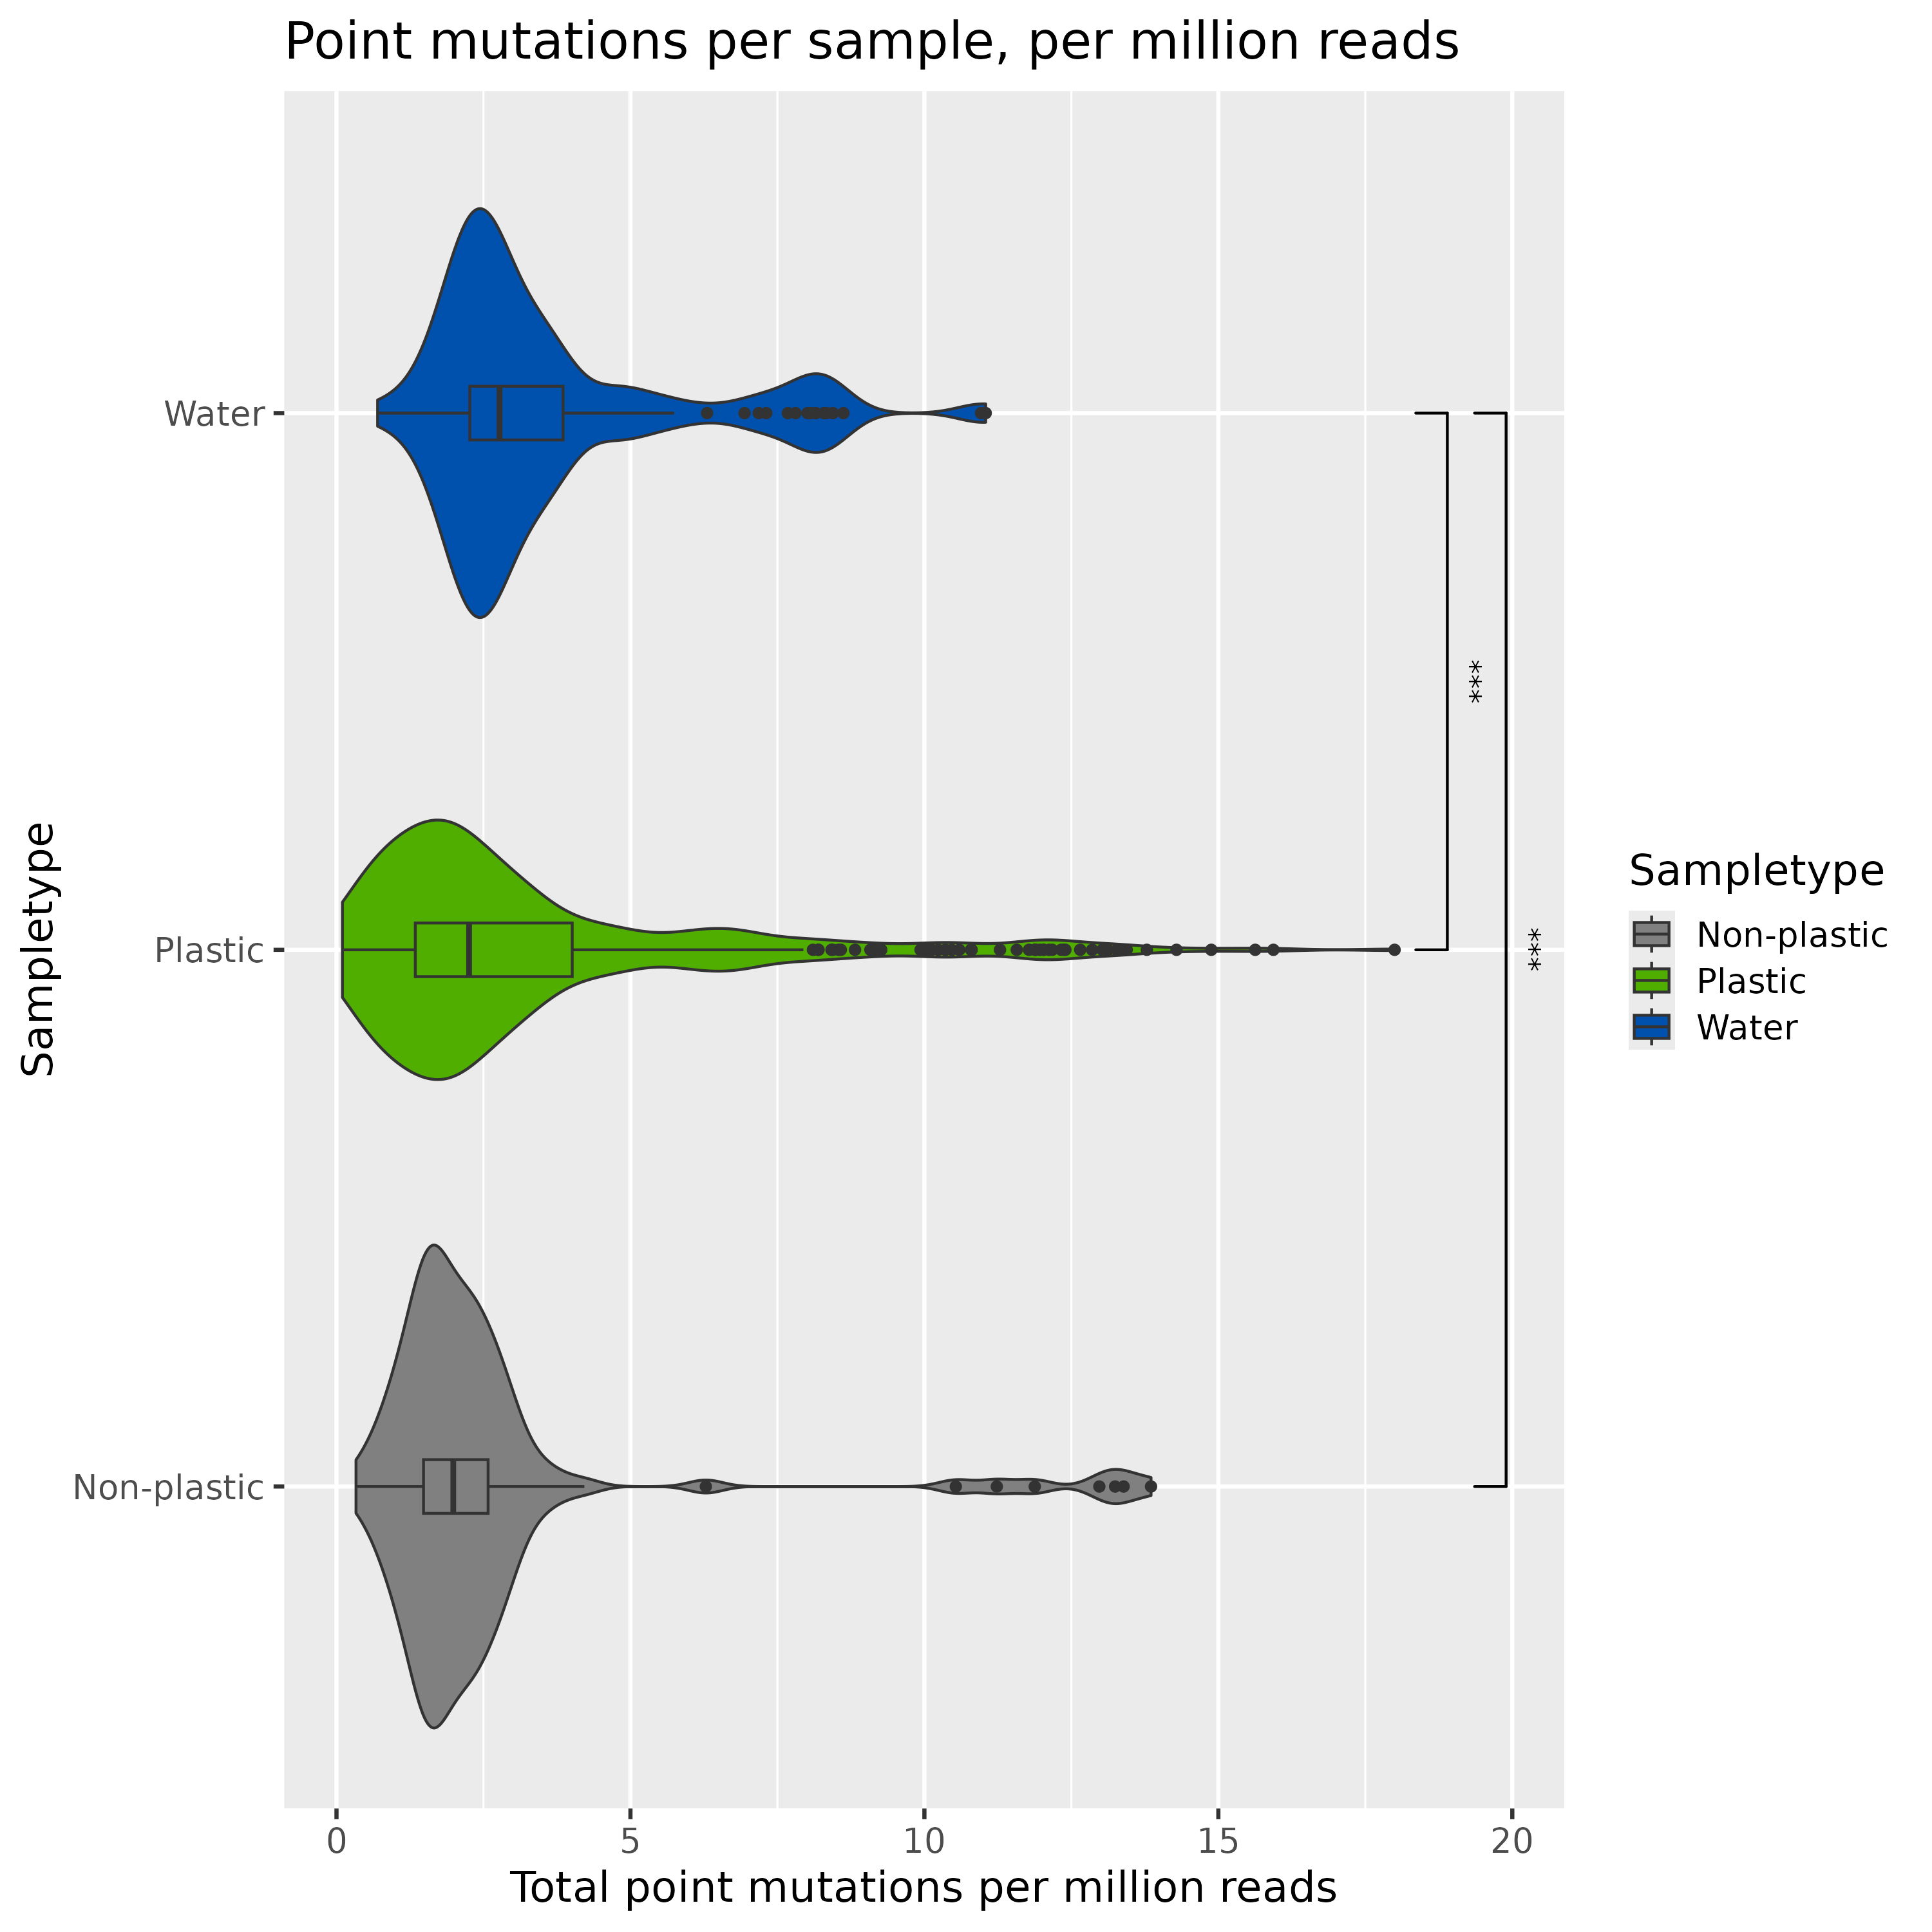
\includegraphics[width = 0.7\textwidth]{figure/hits_per_million_type.png}
    \caption{}
    \label{hits_type}
\end{figure}

The result of grouping the samples by substrate type instead is shown in figure \ref{hits_substrate}, which show that there can be a great difference in total hit count per million between different substrate types. 
Figure \ref{wilcox_hits_substrate} show the statistical significance of the comparison, where a wilcoxon test was done for the Substrate versus the Reference. The figure also shows the sign of the pseudo-mean for the comparison, labelled "Change", and is set to Increase if the pseudo-mean is positive and Decrease if it negative.
Note that all comparisons were done, but only the significant ones (p < 0.05) are shown.
There are some plastic substrates which show an increase compared to most other substrates. These include PFP, Ecovio and BI-OPL. 
The soil substrate also show an increase compared to many other substrates, as does freshwater and seawater, with the exception of the substrates previously mentioned. 
The plastic substrates which show a significant increase compared to the water substrates are PHB, PF, PBAT, LDPE, Ecovio, and BI-OPL. \todo{add full name here and in Acronyms}

% Based on the result in these figures, it is evident that the number of point mutations which confer antibiotic resistance are not more prevalent on all plastics, but instead that specific plastic substrates increase this count.
% These substrates include PFP, Ecovio, and BI-OPL. The latter two are biodegradable plastics which contain a blend of PBAT and PLA. 

\begin{figure}[h]
    \centering
    \subfloat[caption1.\label{hits_substrate}]{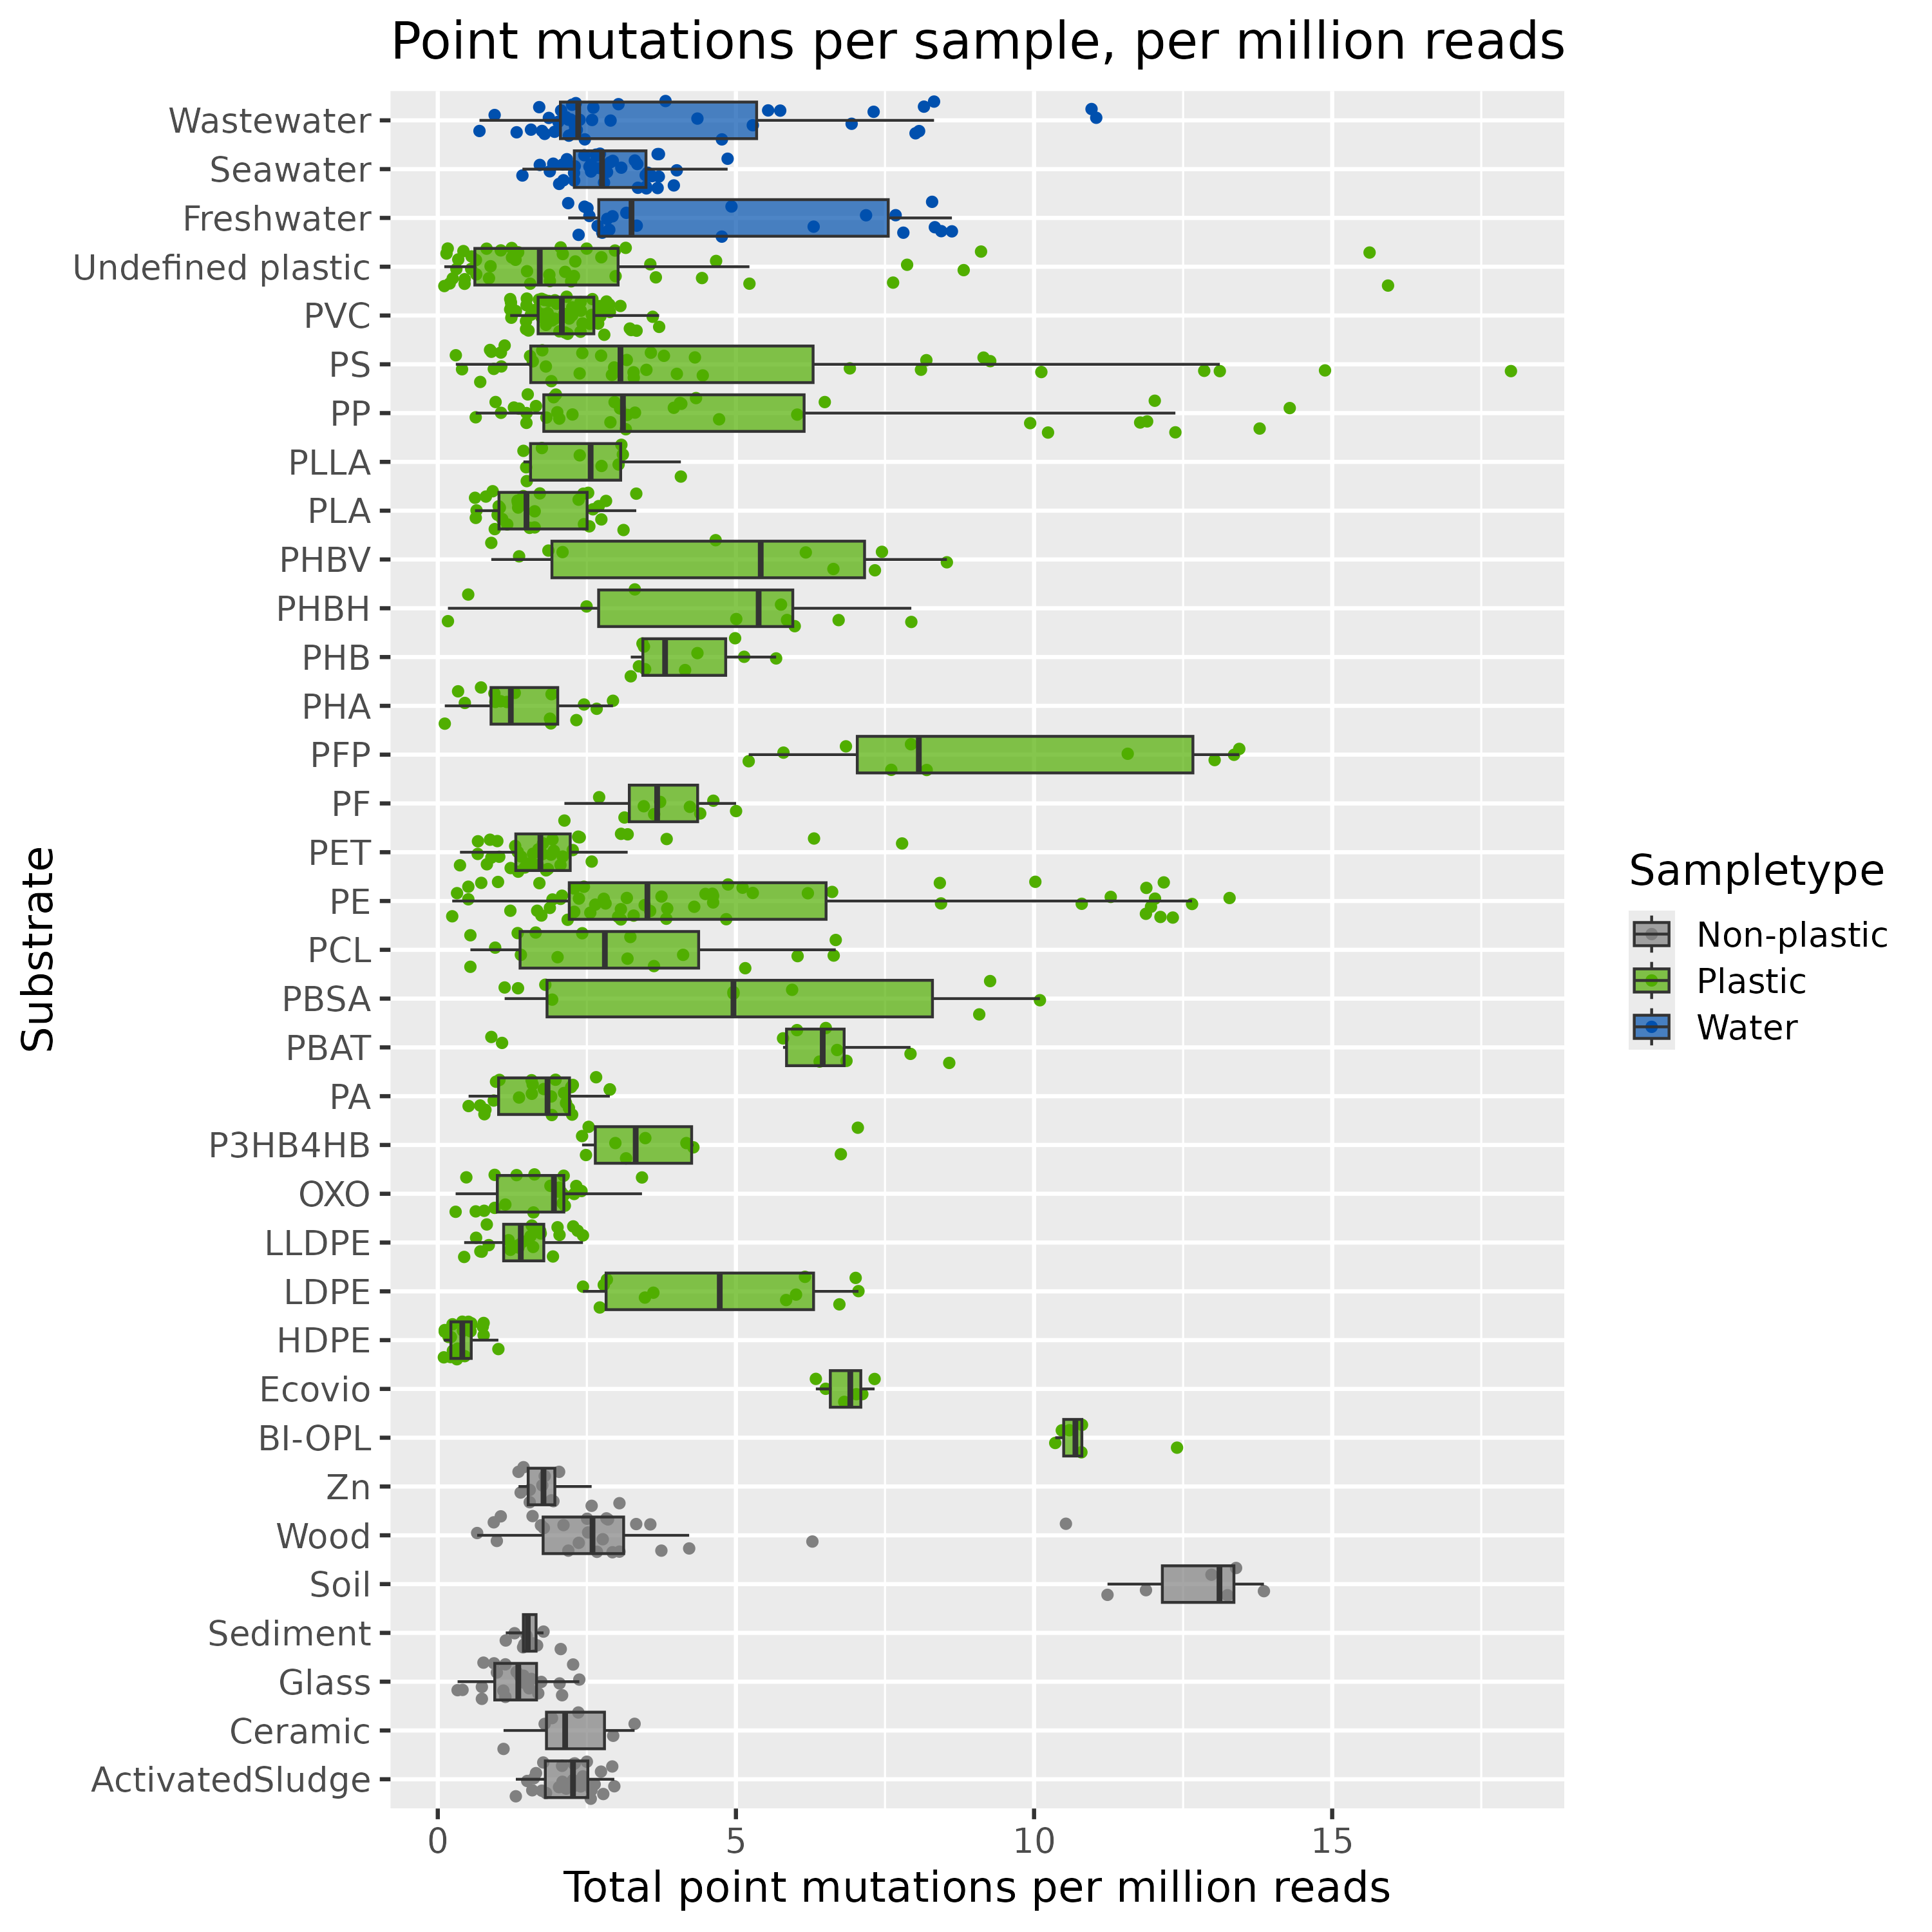
\includegraphics[width=0.5\textwidth]{figure/hits_per_million_substrate.png}}
    \subfloat[caption2.\label{wilcox_hits_substrate}]{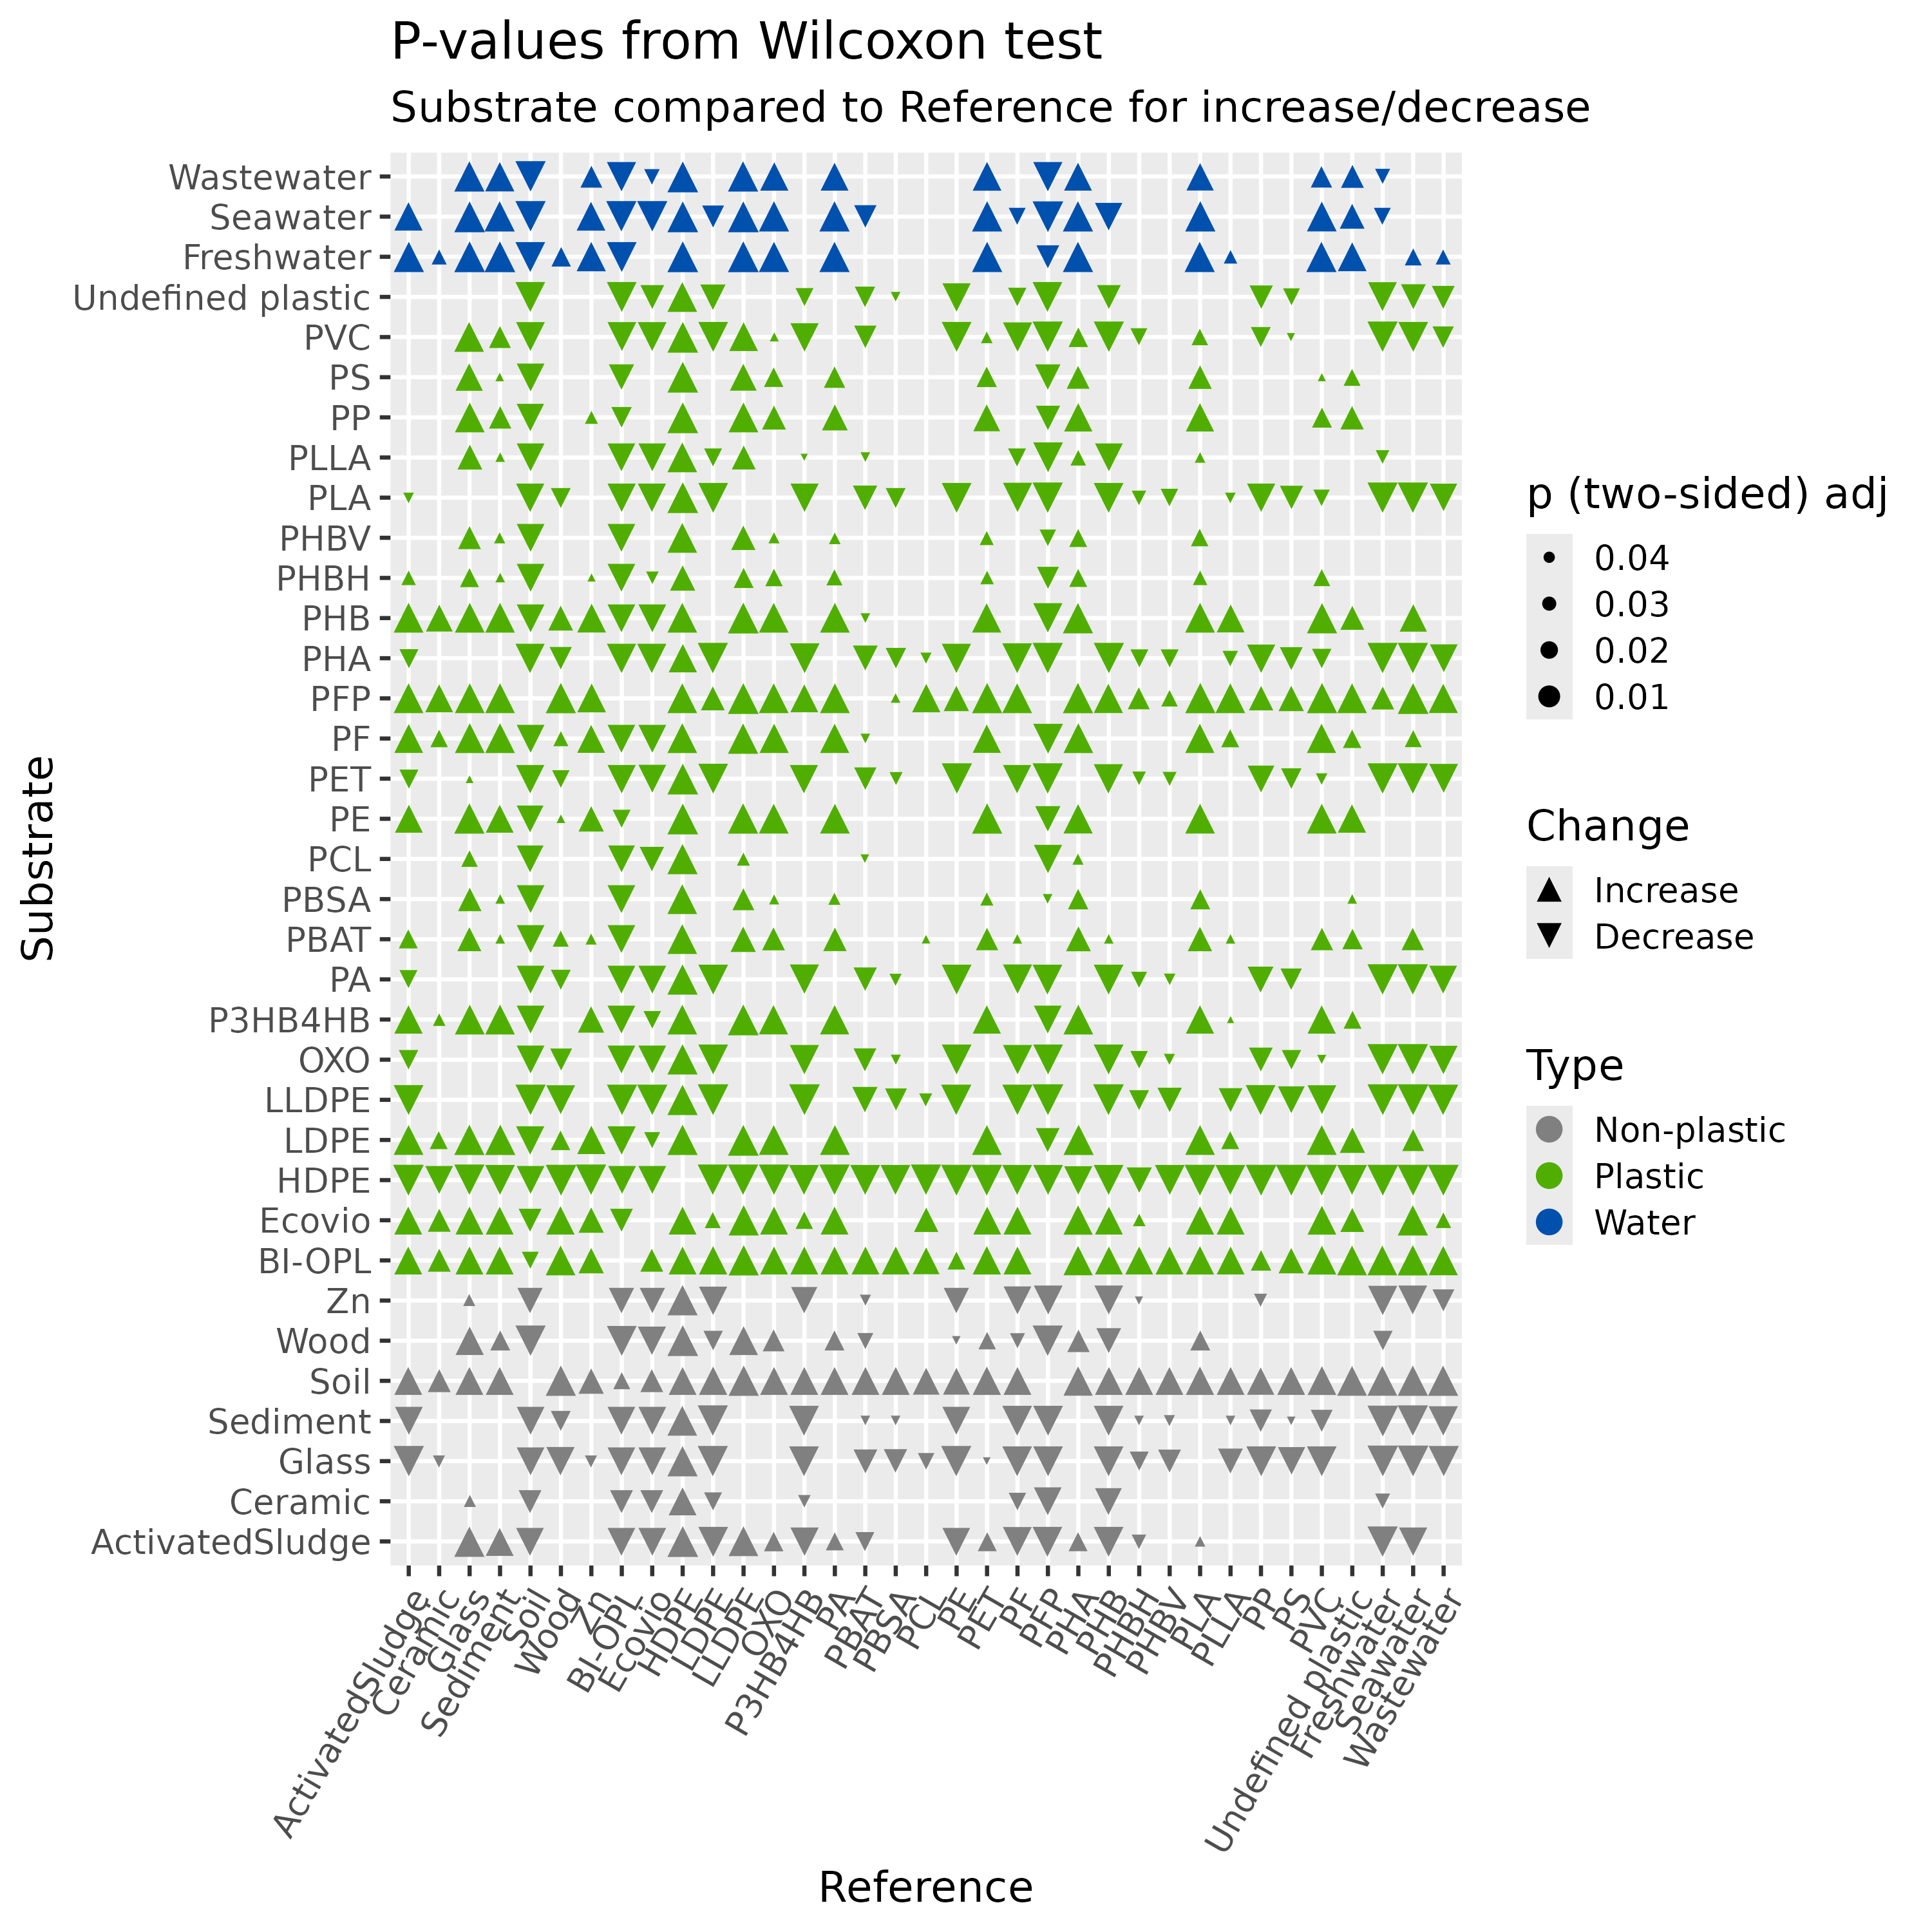
\includegraphics[width=0.5\textwidth]{figure/wilcox_hits_substrates.png}}
    \caption{Total Hits Substrate}
    \label{both_hits_substrate}
\end{figure}


\section{Mean percent mutation}
%todo{Mention how the samples are collected, that they take the biofilm and sequence that? Check in a study what they do}

\subsection{Samples} 
\subsubsection{Alternative 1, combined plots, otherwise two separate larger plots, see \ref{mean_samples_substrate_full} and \ref{wilcox_samples_substrates_full}}
The mean mutation percentage was calculated for every sample, and figure \ref{mean_samples_sampletype} show these values grouped by the type of sample.
There is a significant difference between the water group and the plastic group, as well as between the plastic group and the non-plastic group. 
The plastic group has a lower mean mutation percentage in comparison to both the water group and the non-plastic group. There is no significant difference between the mean mutation percentage for the water group and the non-plastic group.


\todo{Remove n.s.?}
\begin{figure}[h]
    \centering
    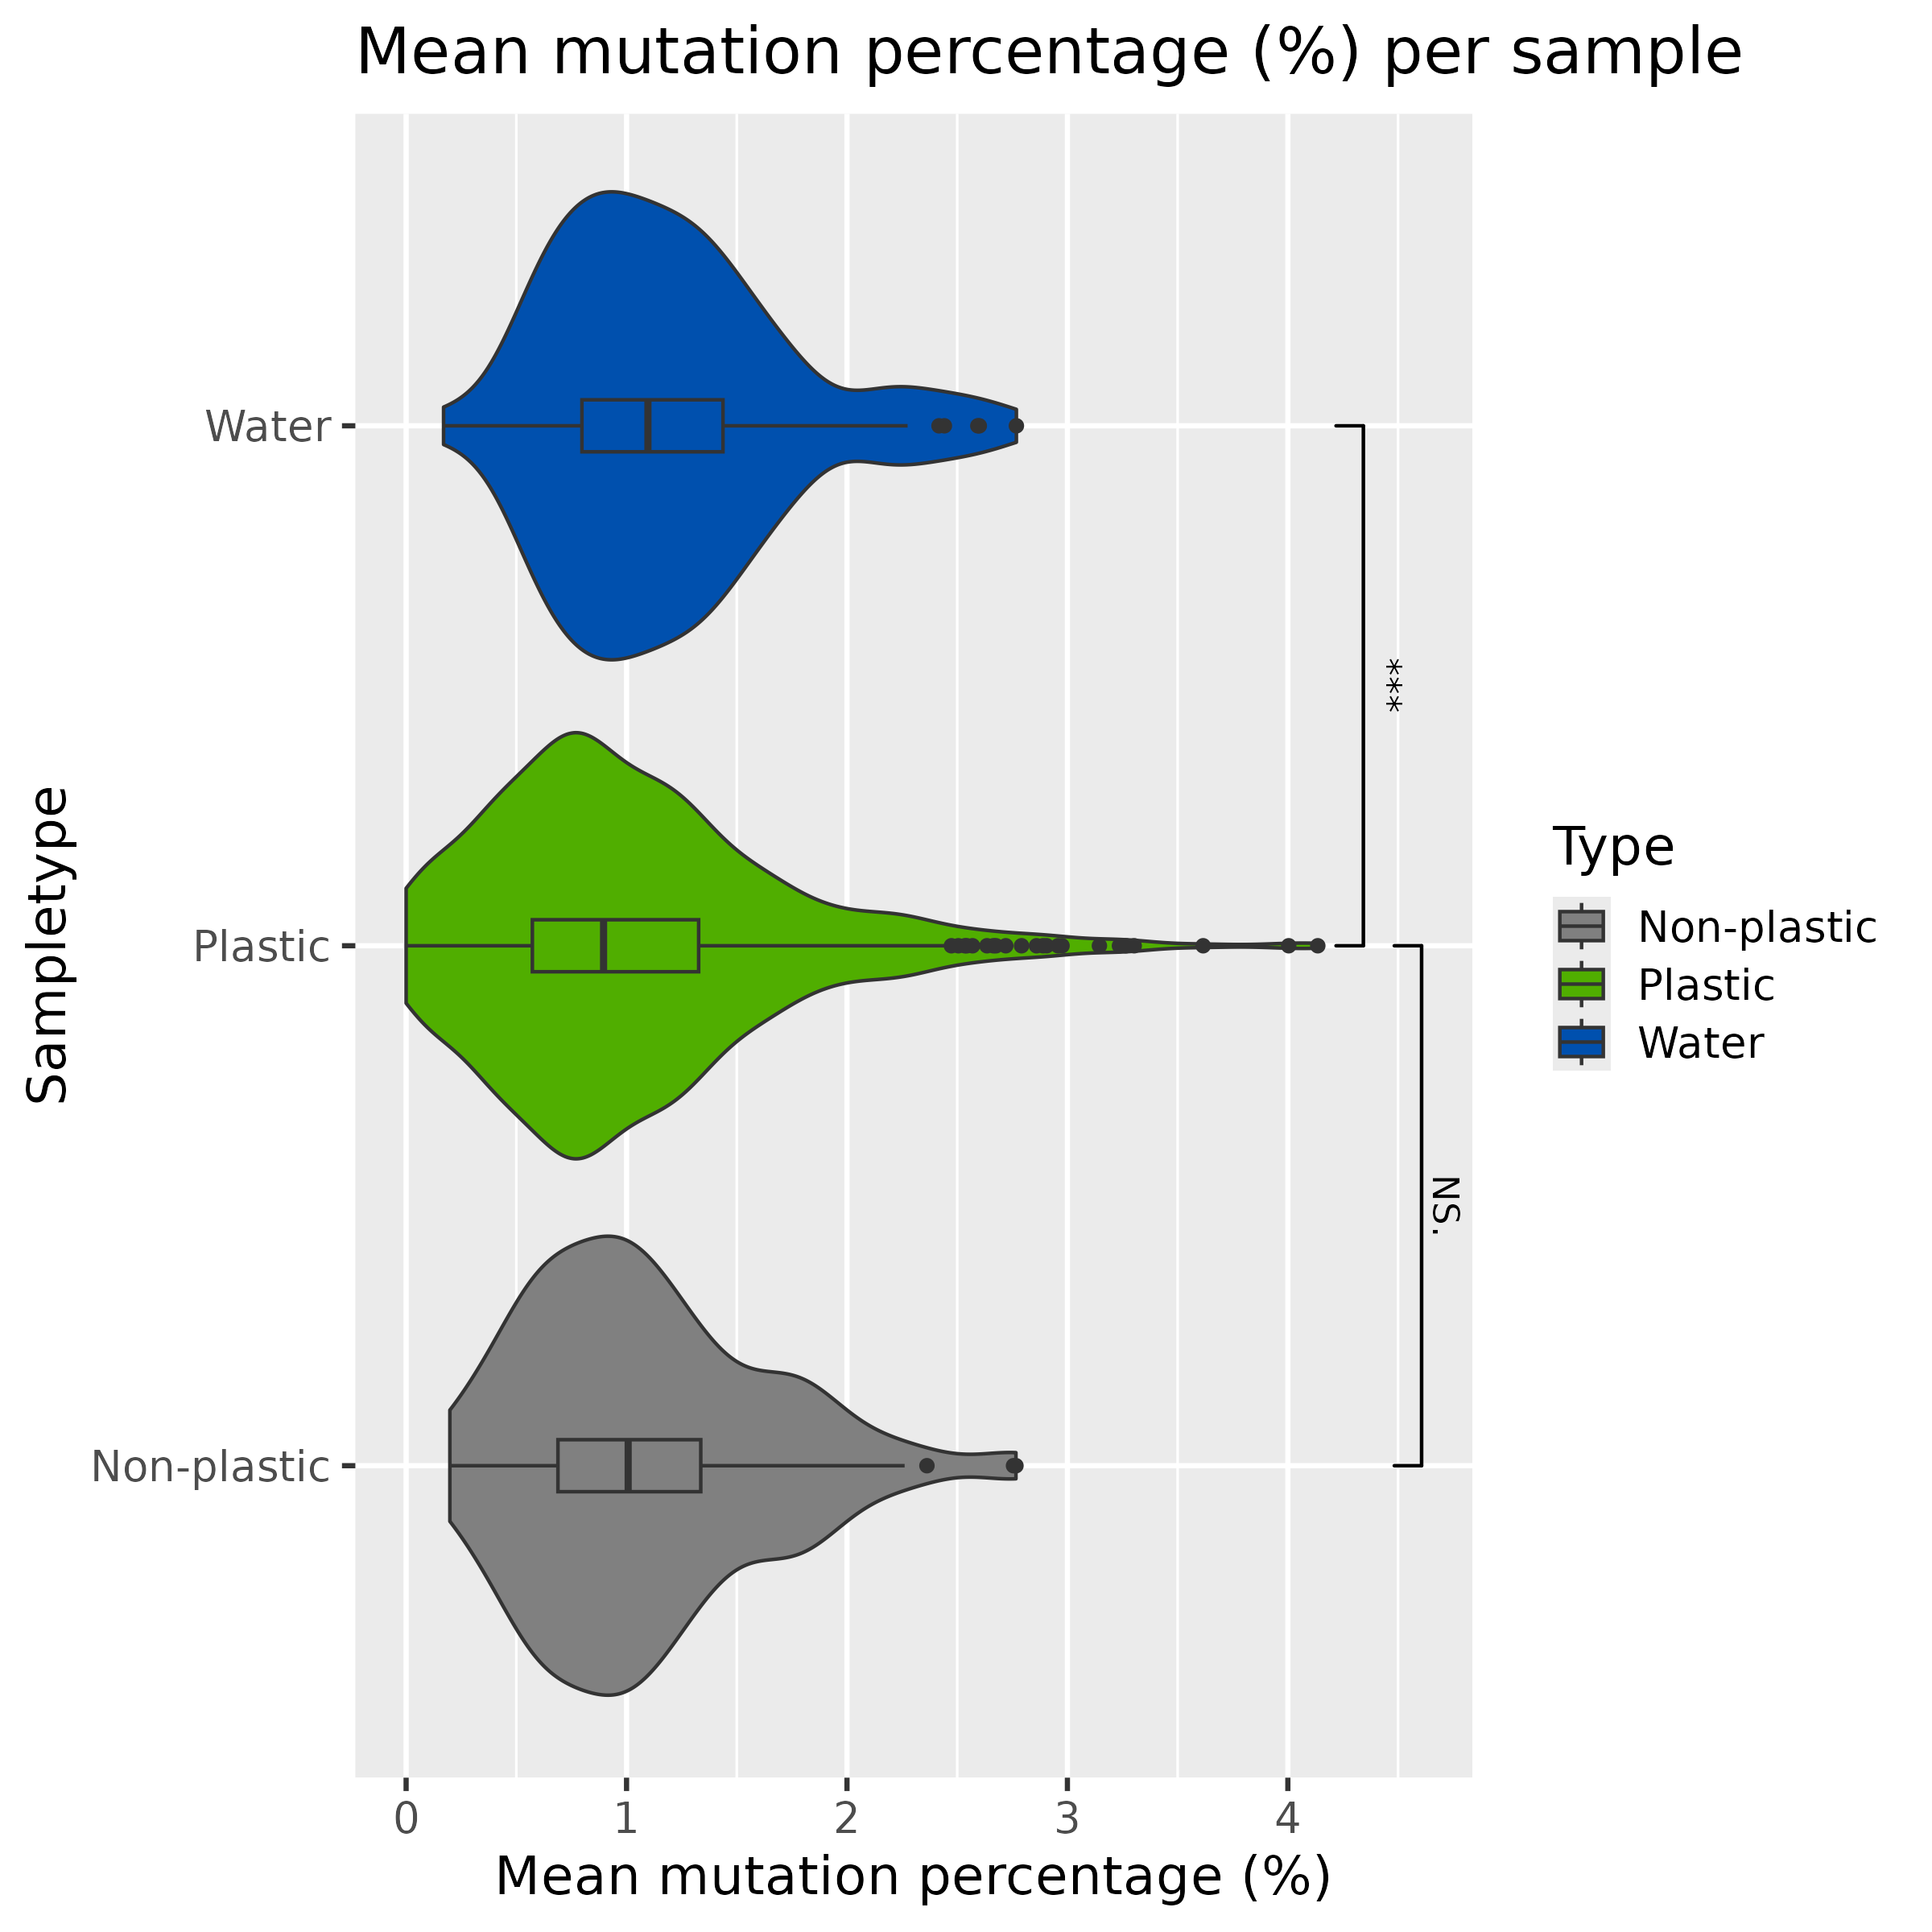
\includegraphics[width = 0.7\textwidth]{figure/mean_samples_sampletype.png}
    \caption{Mean mutation percentage (\%) per sample, grouped by sampletype. * = p < 0.05, *** = p < 0.001}
    \label{mean_samples_sampletype}
\end{figure}
\todo{P-values-table in appendix or not at all?)}

\begin{table}[h]
\caption{p-values from Wilcoxon test between sampletypes}
\label{wilcox_samples_sampletype}
\begin{tabular}{@{}llllll@{}}
\toprule
Sampletype A & Sampletype B & Significance & Change   & p (two-sided) & pseudo\_mean  \\ \midrule
Non-plastic  & Plastic      & *            & Increase & 0.0473  &  0.0012  \\
Water        & Plastic      & ***          & Increase & 0.0005  &  0.0020  \\
Non-plastic  & Water        & ns           & Decrease & 0.1801  & -0.0009 \\
Plastic      & Water        & ***          & Decrease & 0.0005  & -0.0020 \\
Plastic      & Non-plastic  & *            & Decrease & 0.0473  & -0.0012 \\
Water        & Non-plastic  & ns           & Increase & 0.1801  &  0.0009 \\ \bottomrule
\end{tabular}
\end{table}


In figure \ref{mean_samples_substrate} the samples are instead grouped by substrate type, which shows that there are differences for different plastics, as well as other substrates.
Figure \ref{wilcox_samples_substrate} show the statistical significance of the comparison, when a wilcoxon test was done for the Substrate versus the Reference, as well as if there is an increase of the pseudo-mean compared to the reference.
Note that all comparisons were done, but only the significant ones (p < 0.05) are shown.
It is shown that there are some plastics that has a significant higher mean mutation percentage than most other substrates. These include PFP, LDPE, Ecovio and BI-OPL. The last two plastics are biodegradable plastics. \todo{full names + in Acronyms}
The plastic substrates that has a significant higher mean mutation percentage than seawater or wastewater include PVC and PF in addition to the other plastics mentioned before.
There are also some plastics which have significantly different lower mean mutation percentage than almost all other substrates, the most notable of which is high-density polyethylene (HDPE), poly(3-hydroxybutyrate-co-3-hydroxyvalerate) (PHBV) and polyhydroxyalkanoate (PHA), of which the latter two are biodegradable polymers while the first one is not.
Almost all substrates has a significantly different lower mean mutation percentage than the freshwater samples, the exception of which is leaf, rock, Ecovio, BI-OPL, and PFP where there is no significant difference. 
The soil samples also has a significant higher mean mutation percentage compared to many other substrates. 
%todo{meh, "which is expected from previous studies" + ref? Idk varför det nämns}.


\begin{figure}[h]
    \centering
    \subfloat[caption1.\label{mean_samples_substrate}]{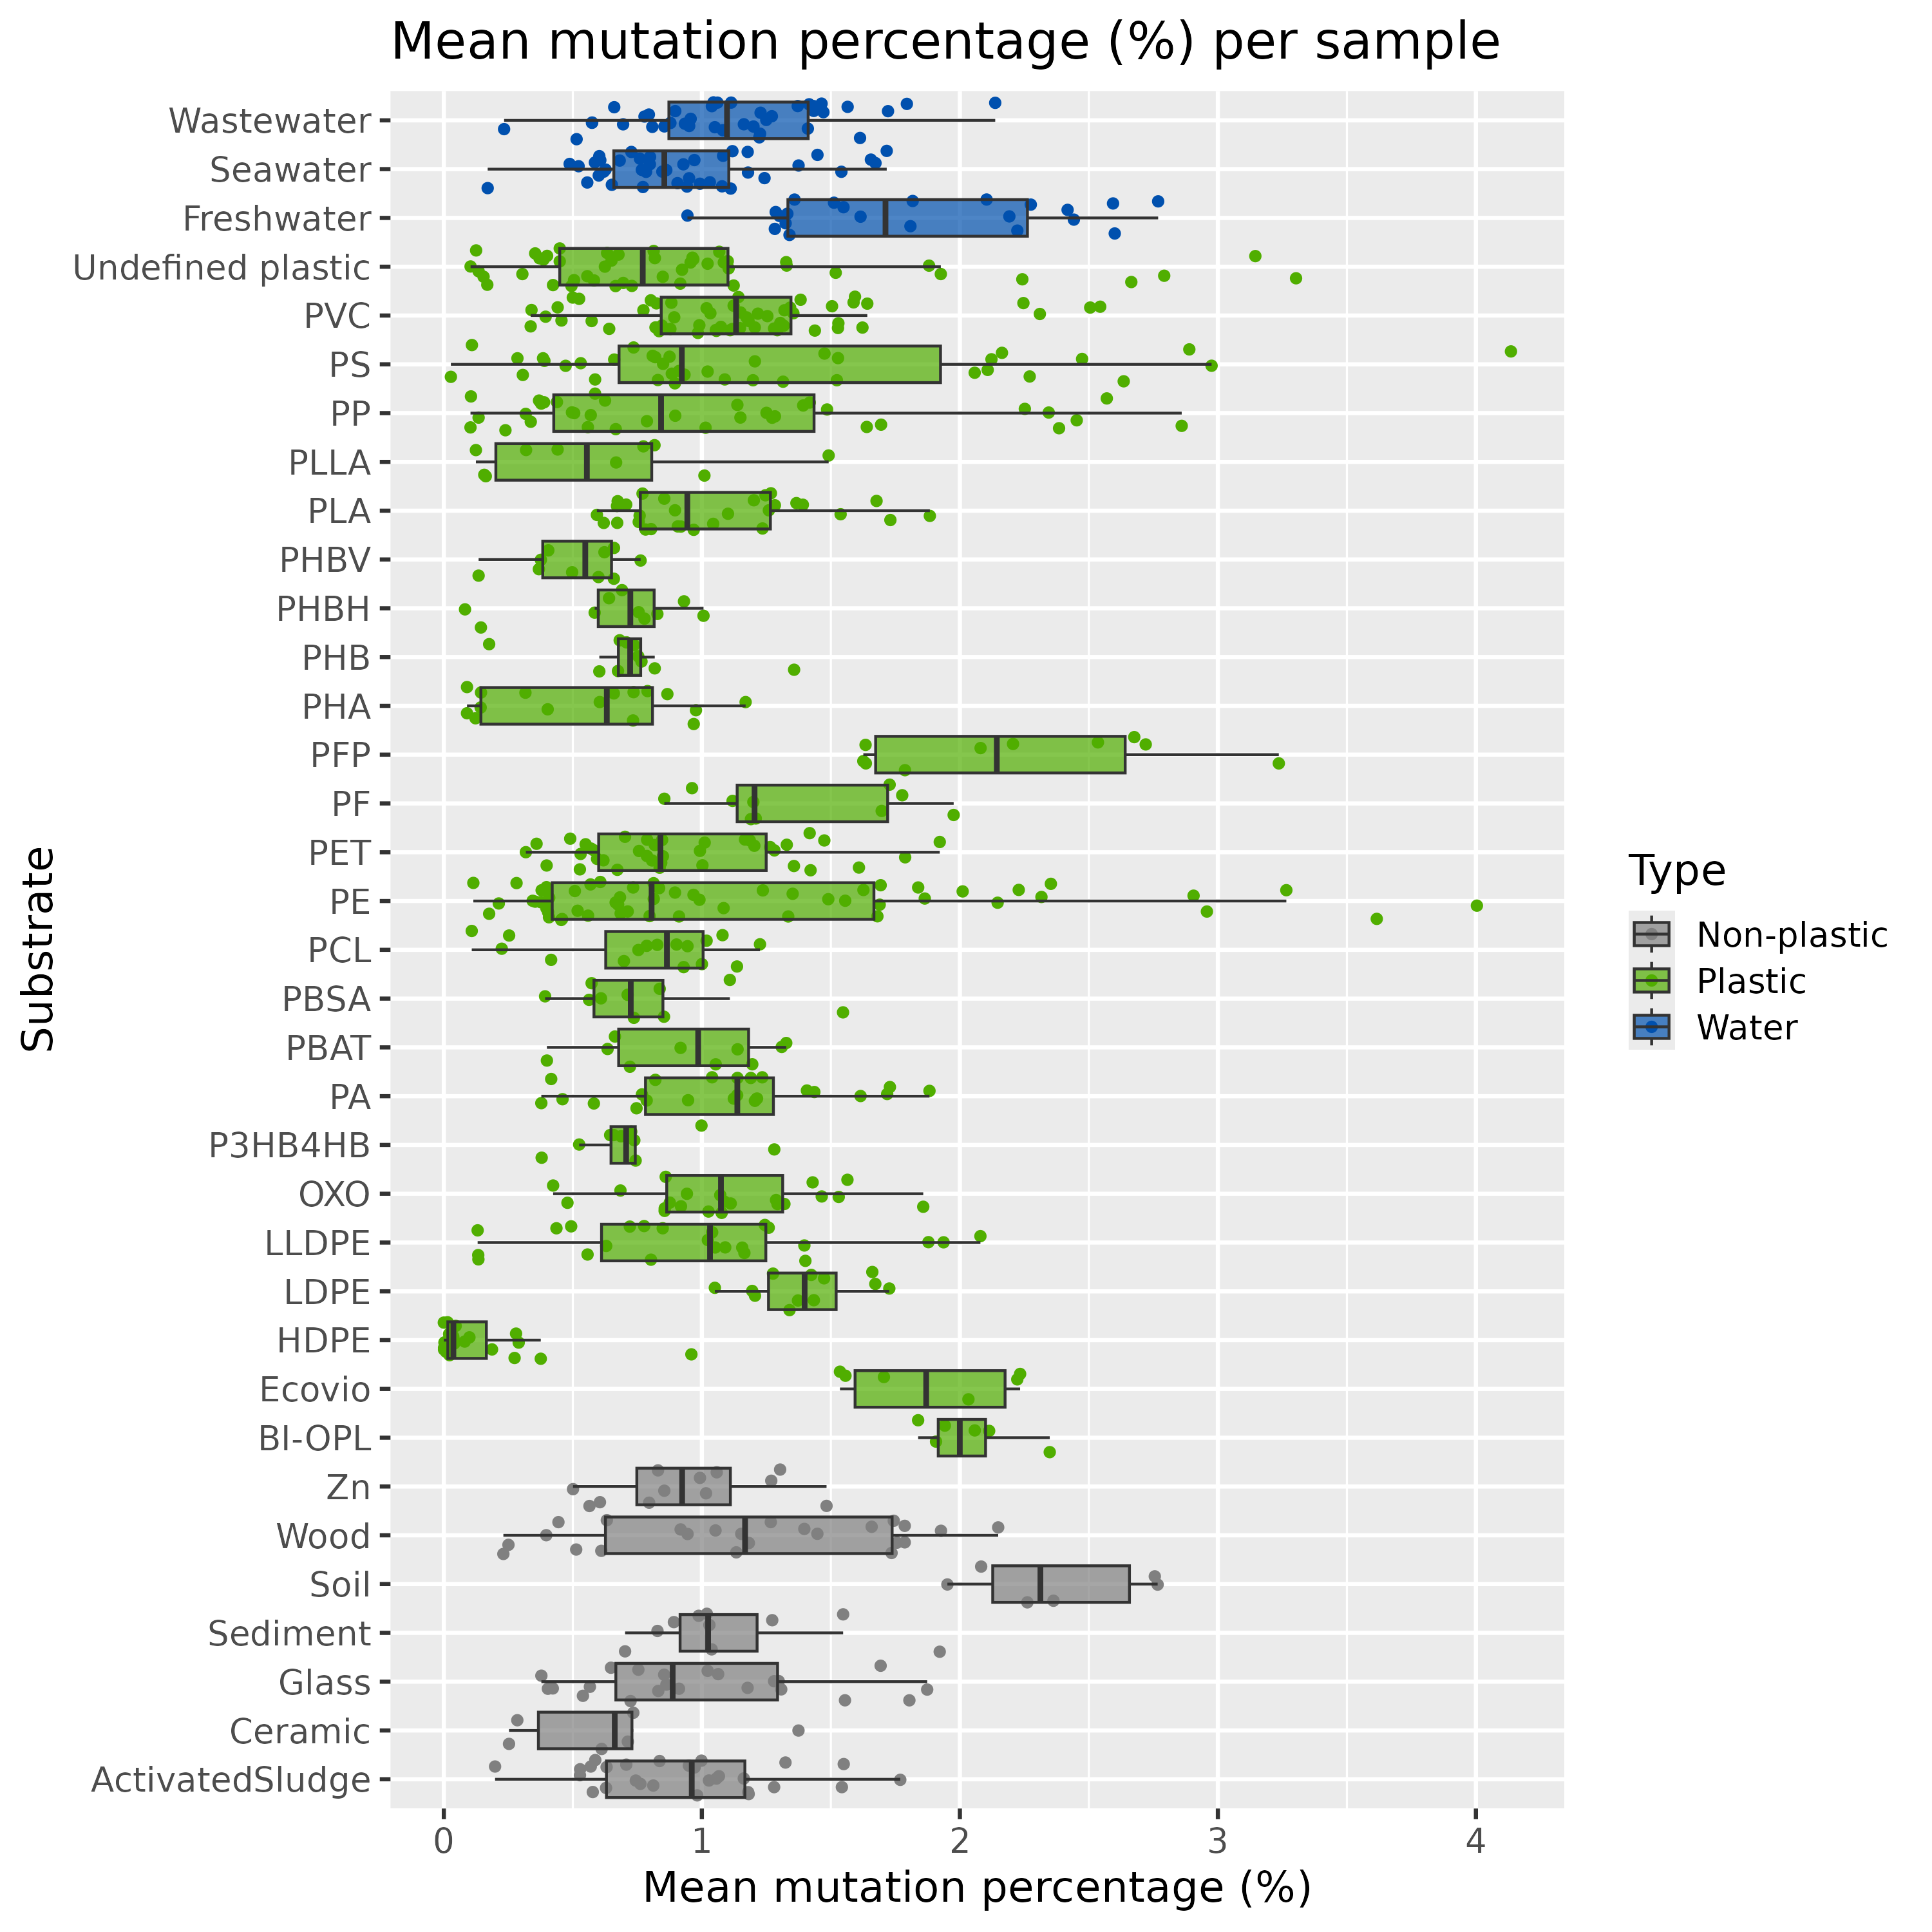
\includegraphics[width=0.5\textwidth]{figure/mean_samples_substrate.png}}
    \subfloat[caption2.\label{wilcox_samples_substrate}]{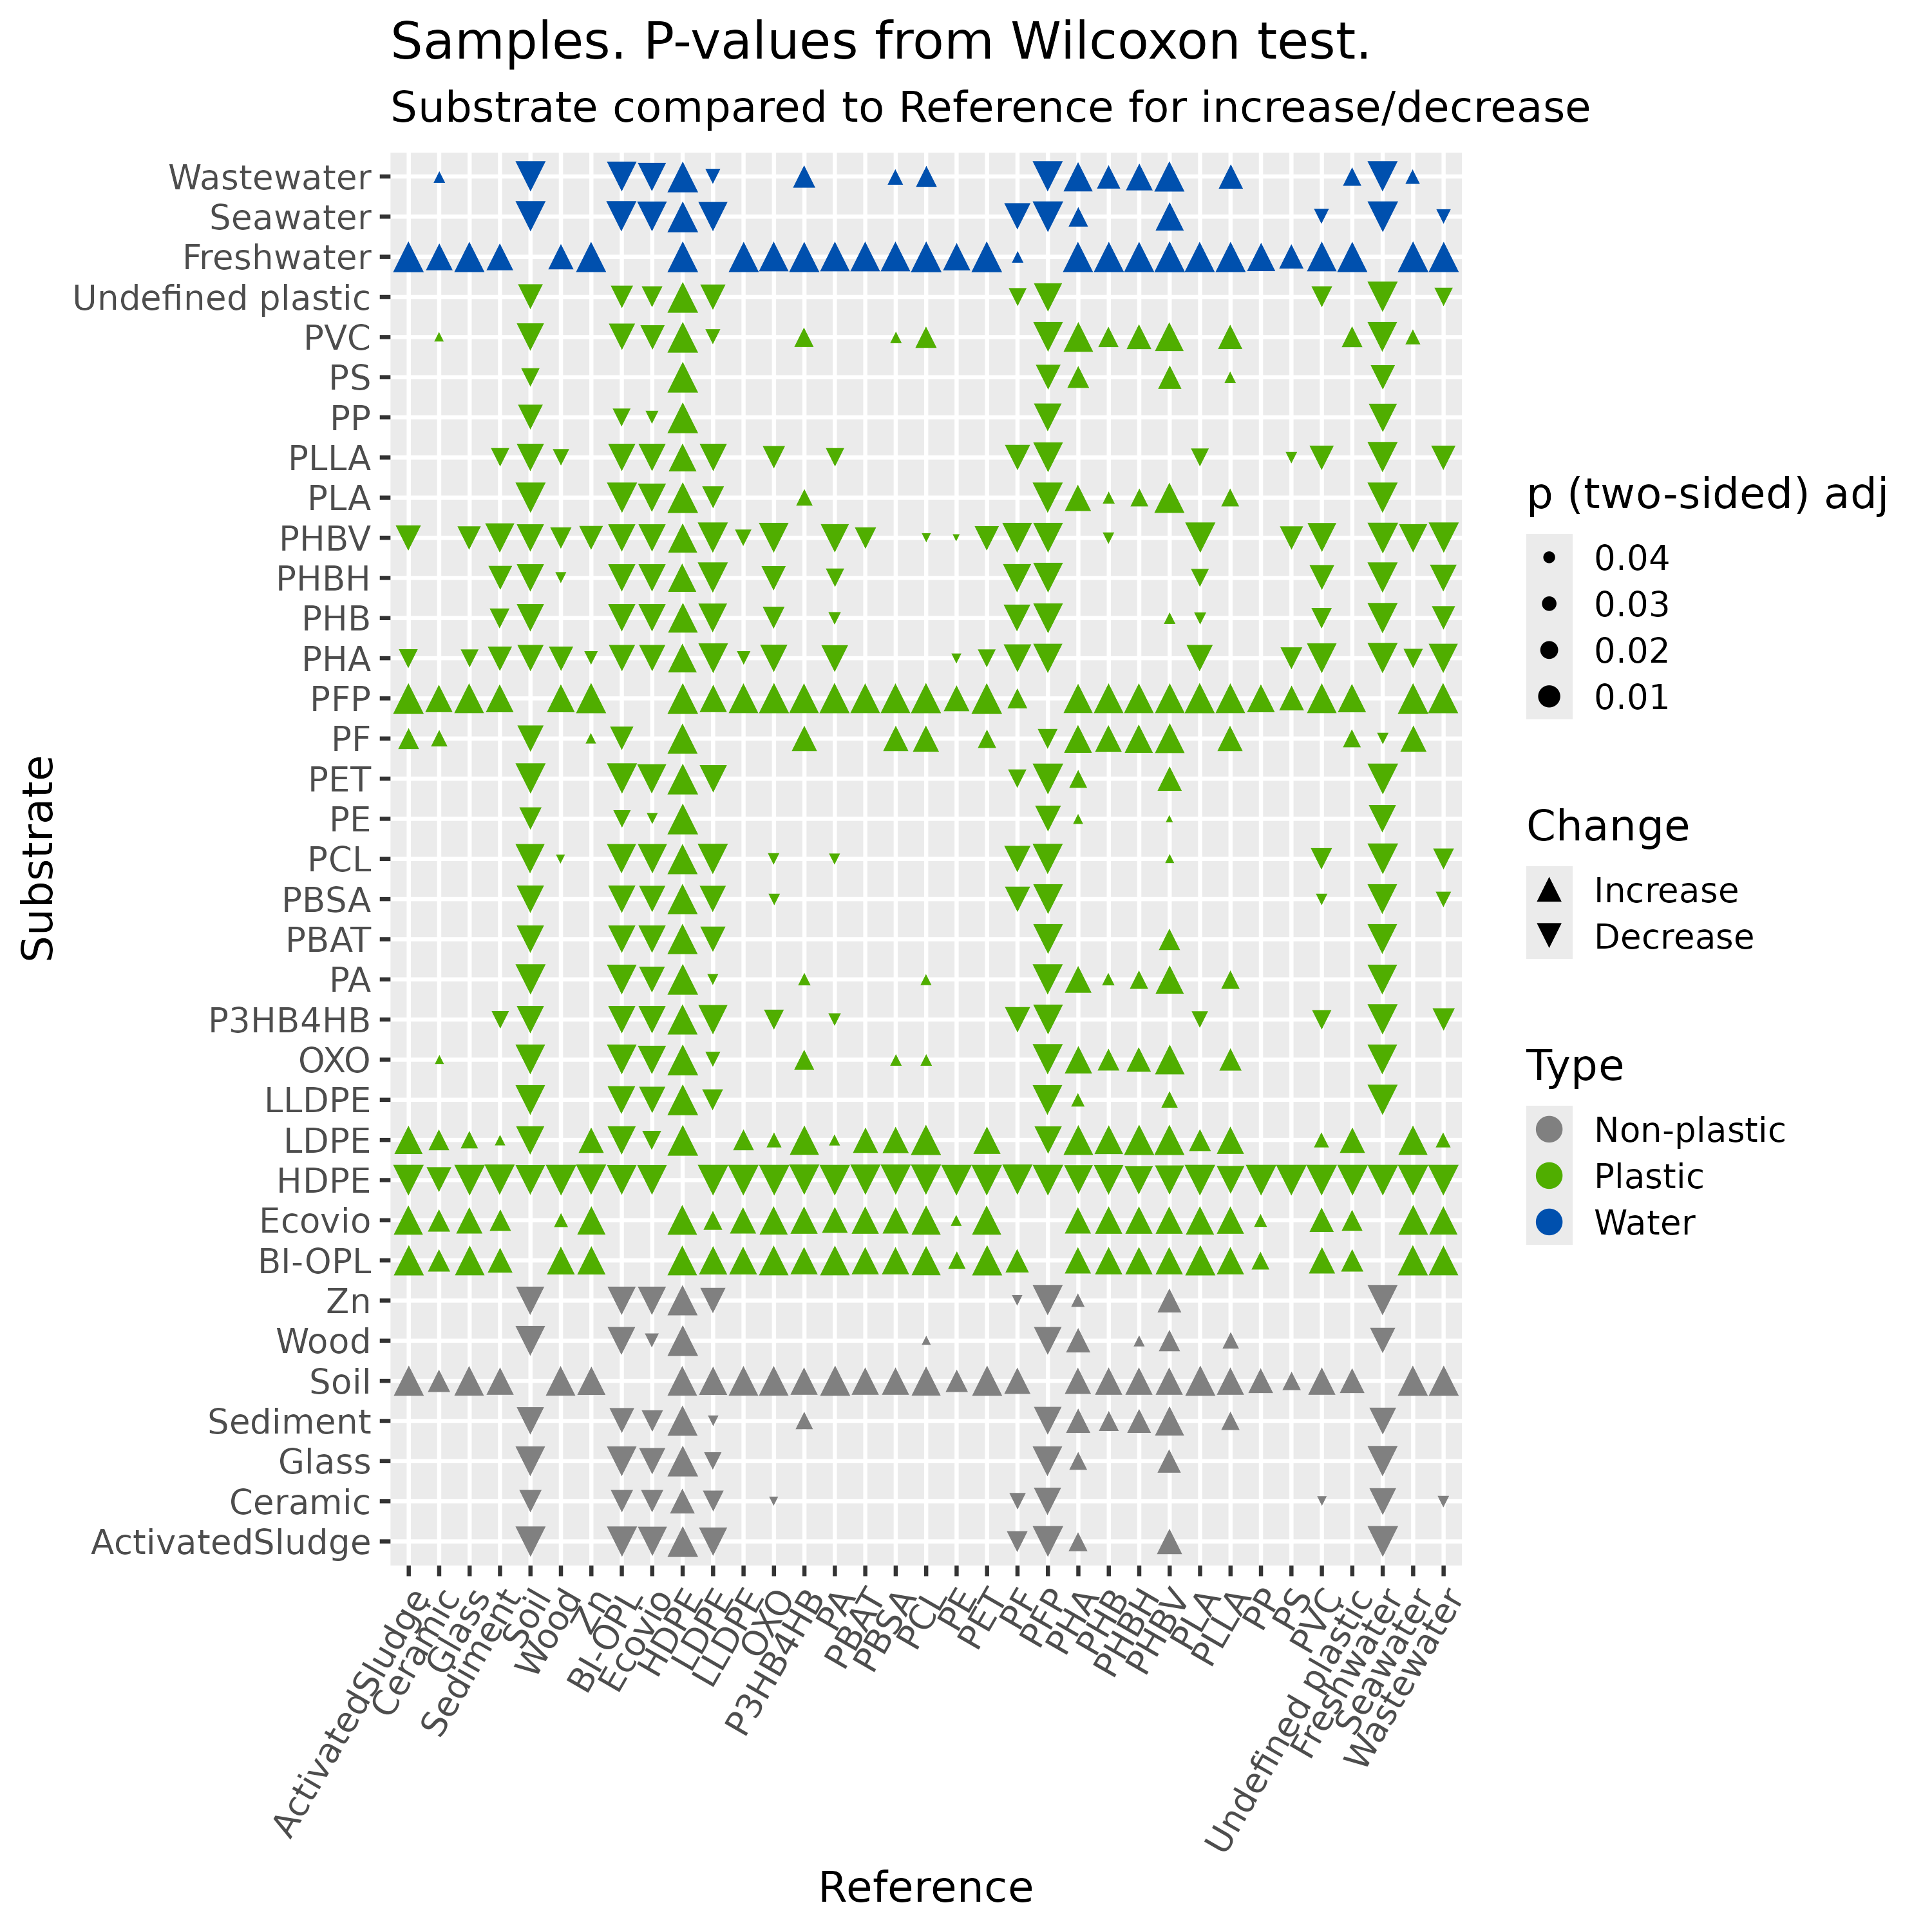
\includegraphics[width=0.5\textwidth]{figure/wilcox_samples_substrates.png}}
    \caption{Mean Samples Substrate}
    \label{both_mean_samples_susbtrates}
\end{figure}

\subsubsection{Alternative 2, separate plots instead of combined, see figure \ref{both_mean_samples_susbtrates}}
\begin{figure}[h]
    \centering
    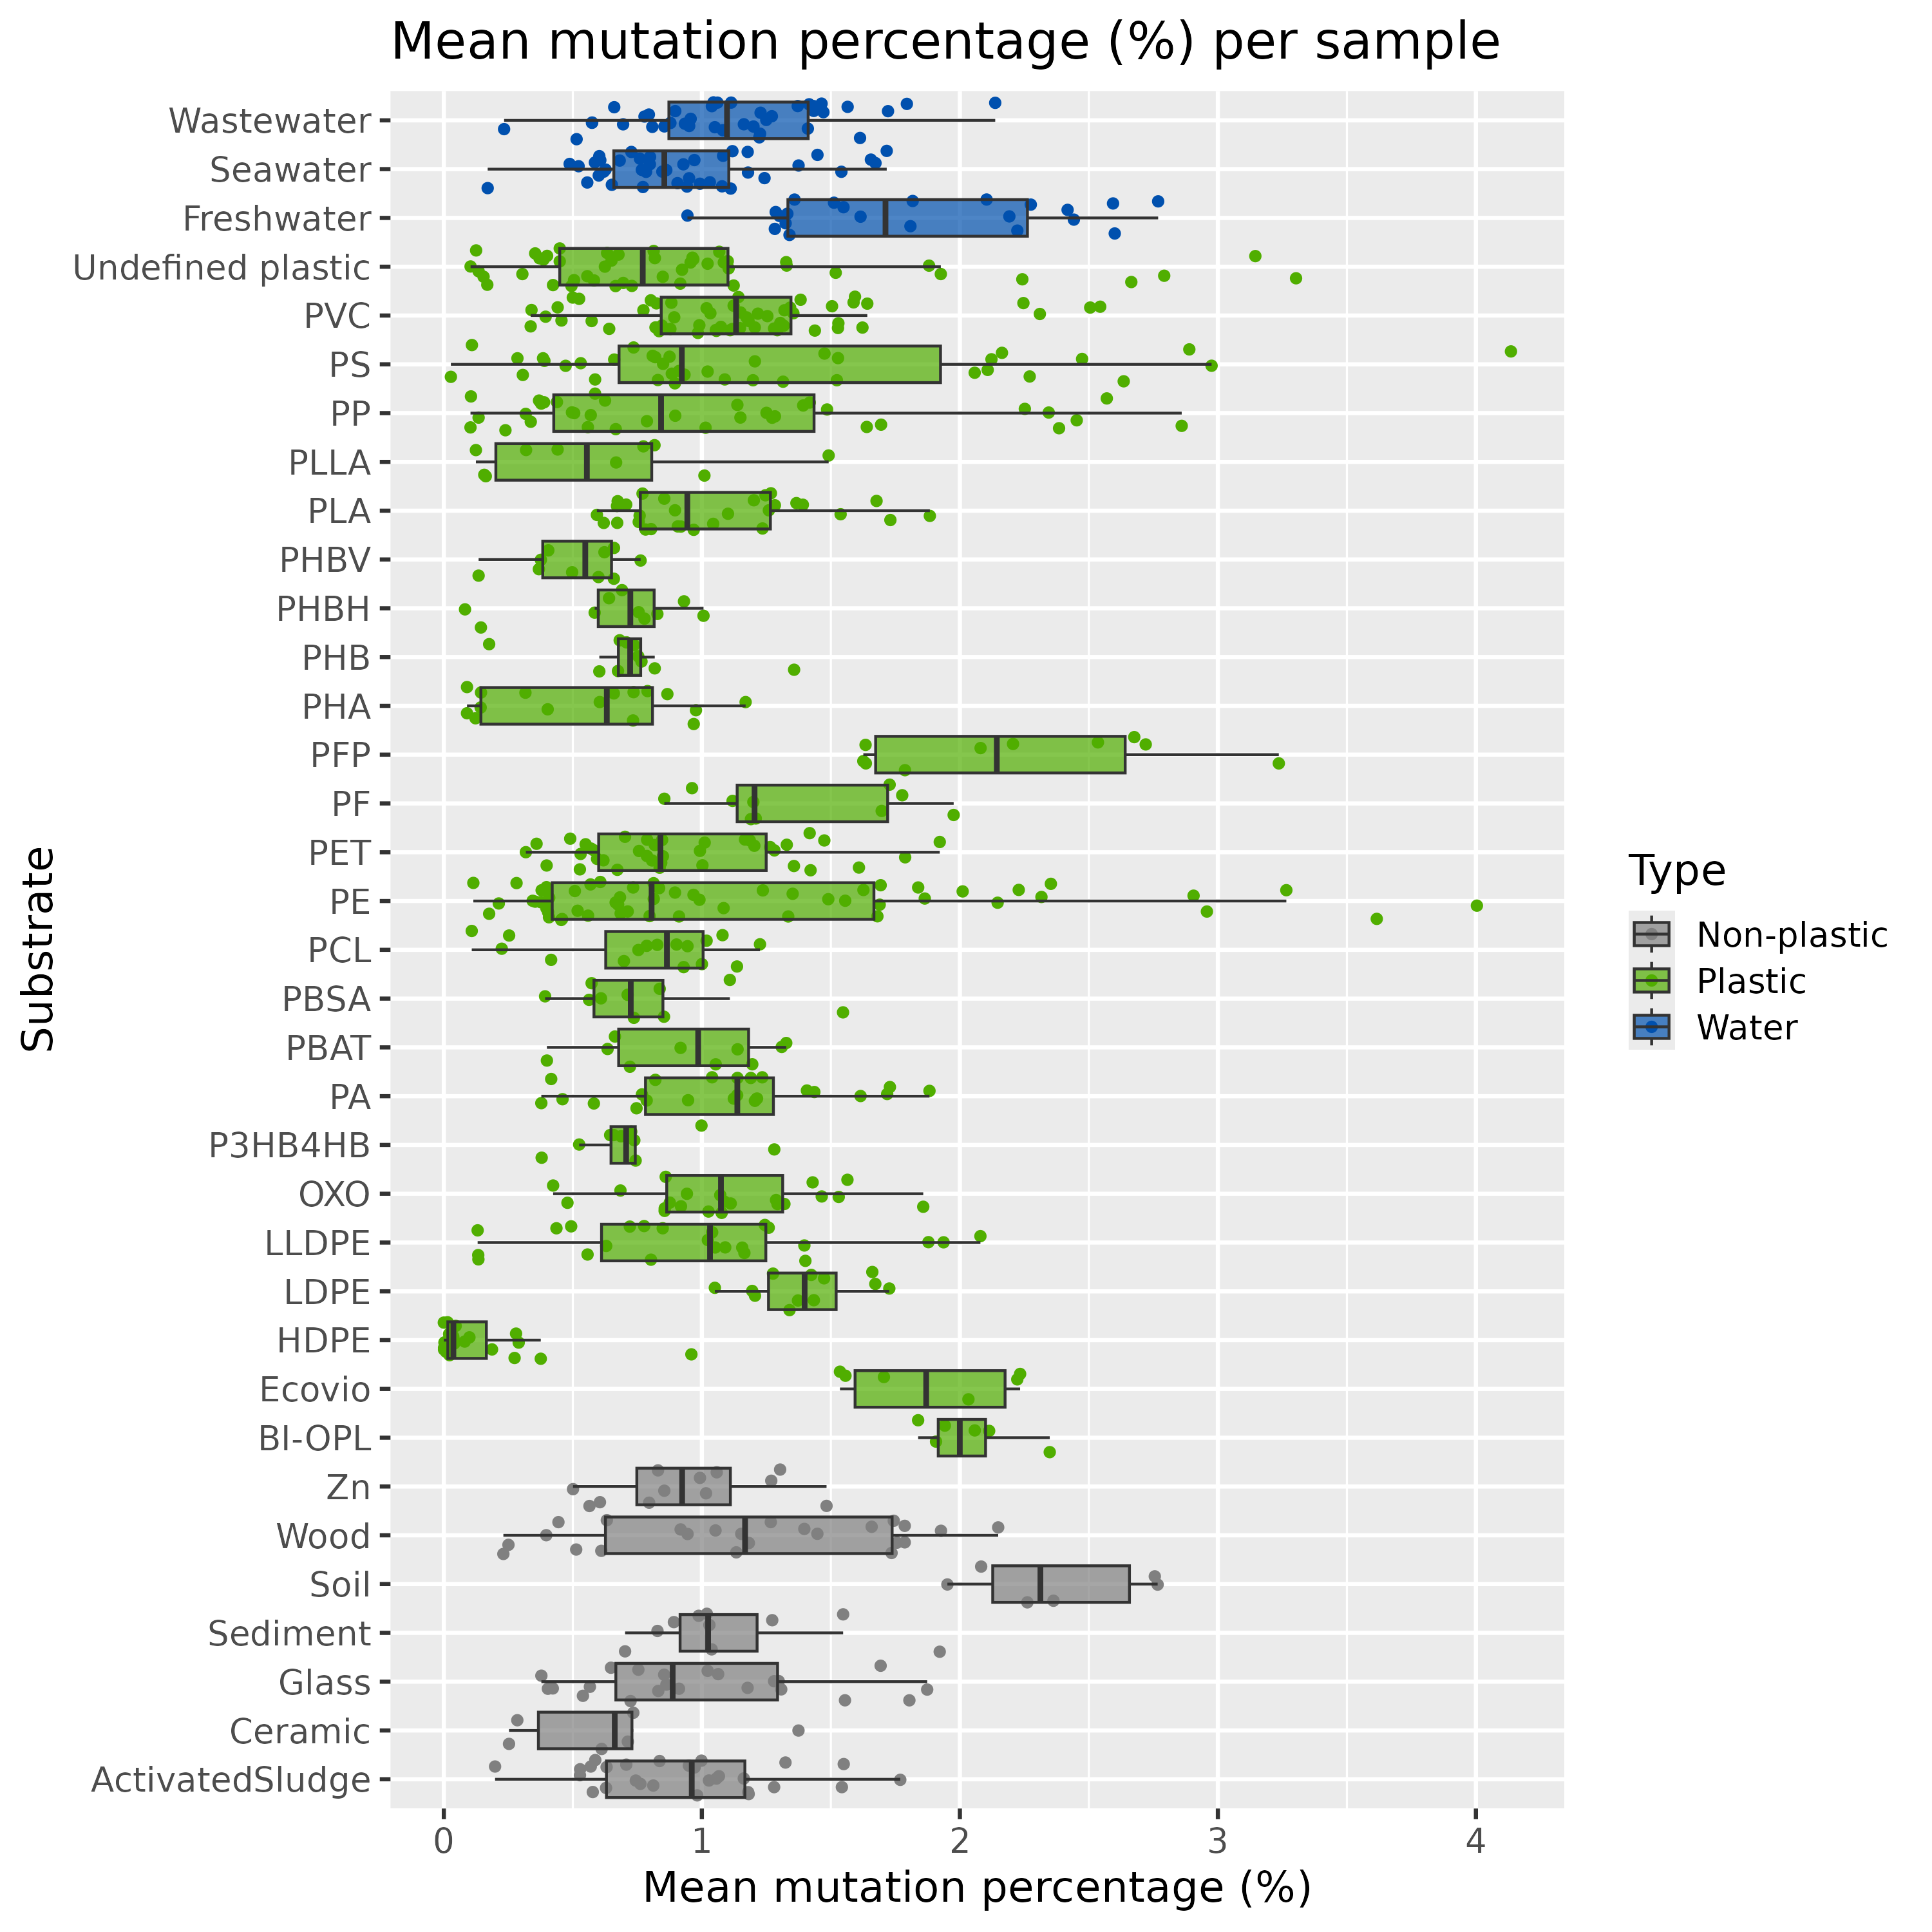
\includegraphics[width = 0.7\textwidth]{figure/mean_samples_substrate.png}
    \caption{Mean Samples Substrate Full}
    \label{mean_samples_substrate_full}
\end{figure}

\begin{figure}[h]
    \centering
    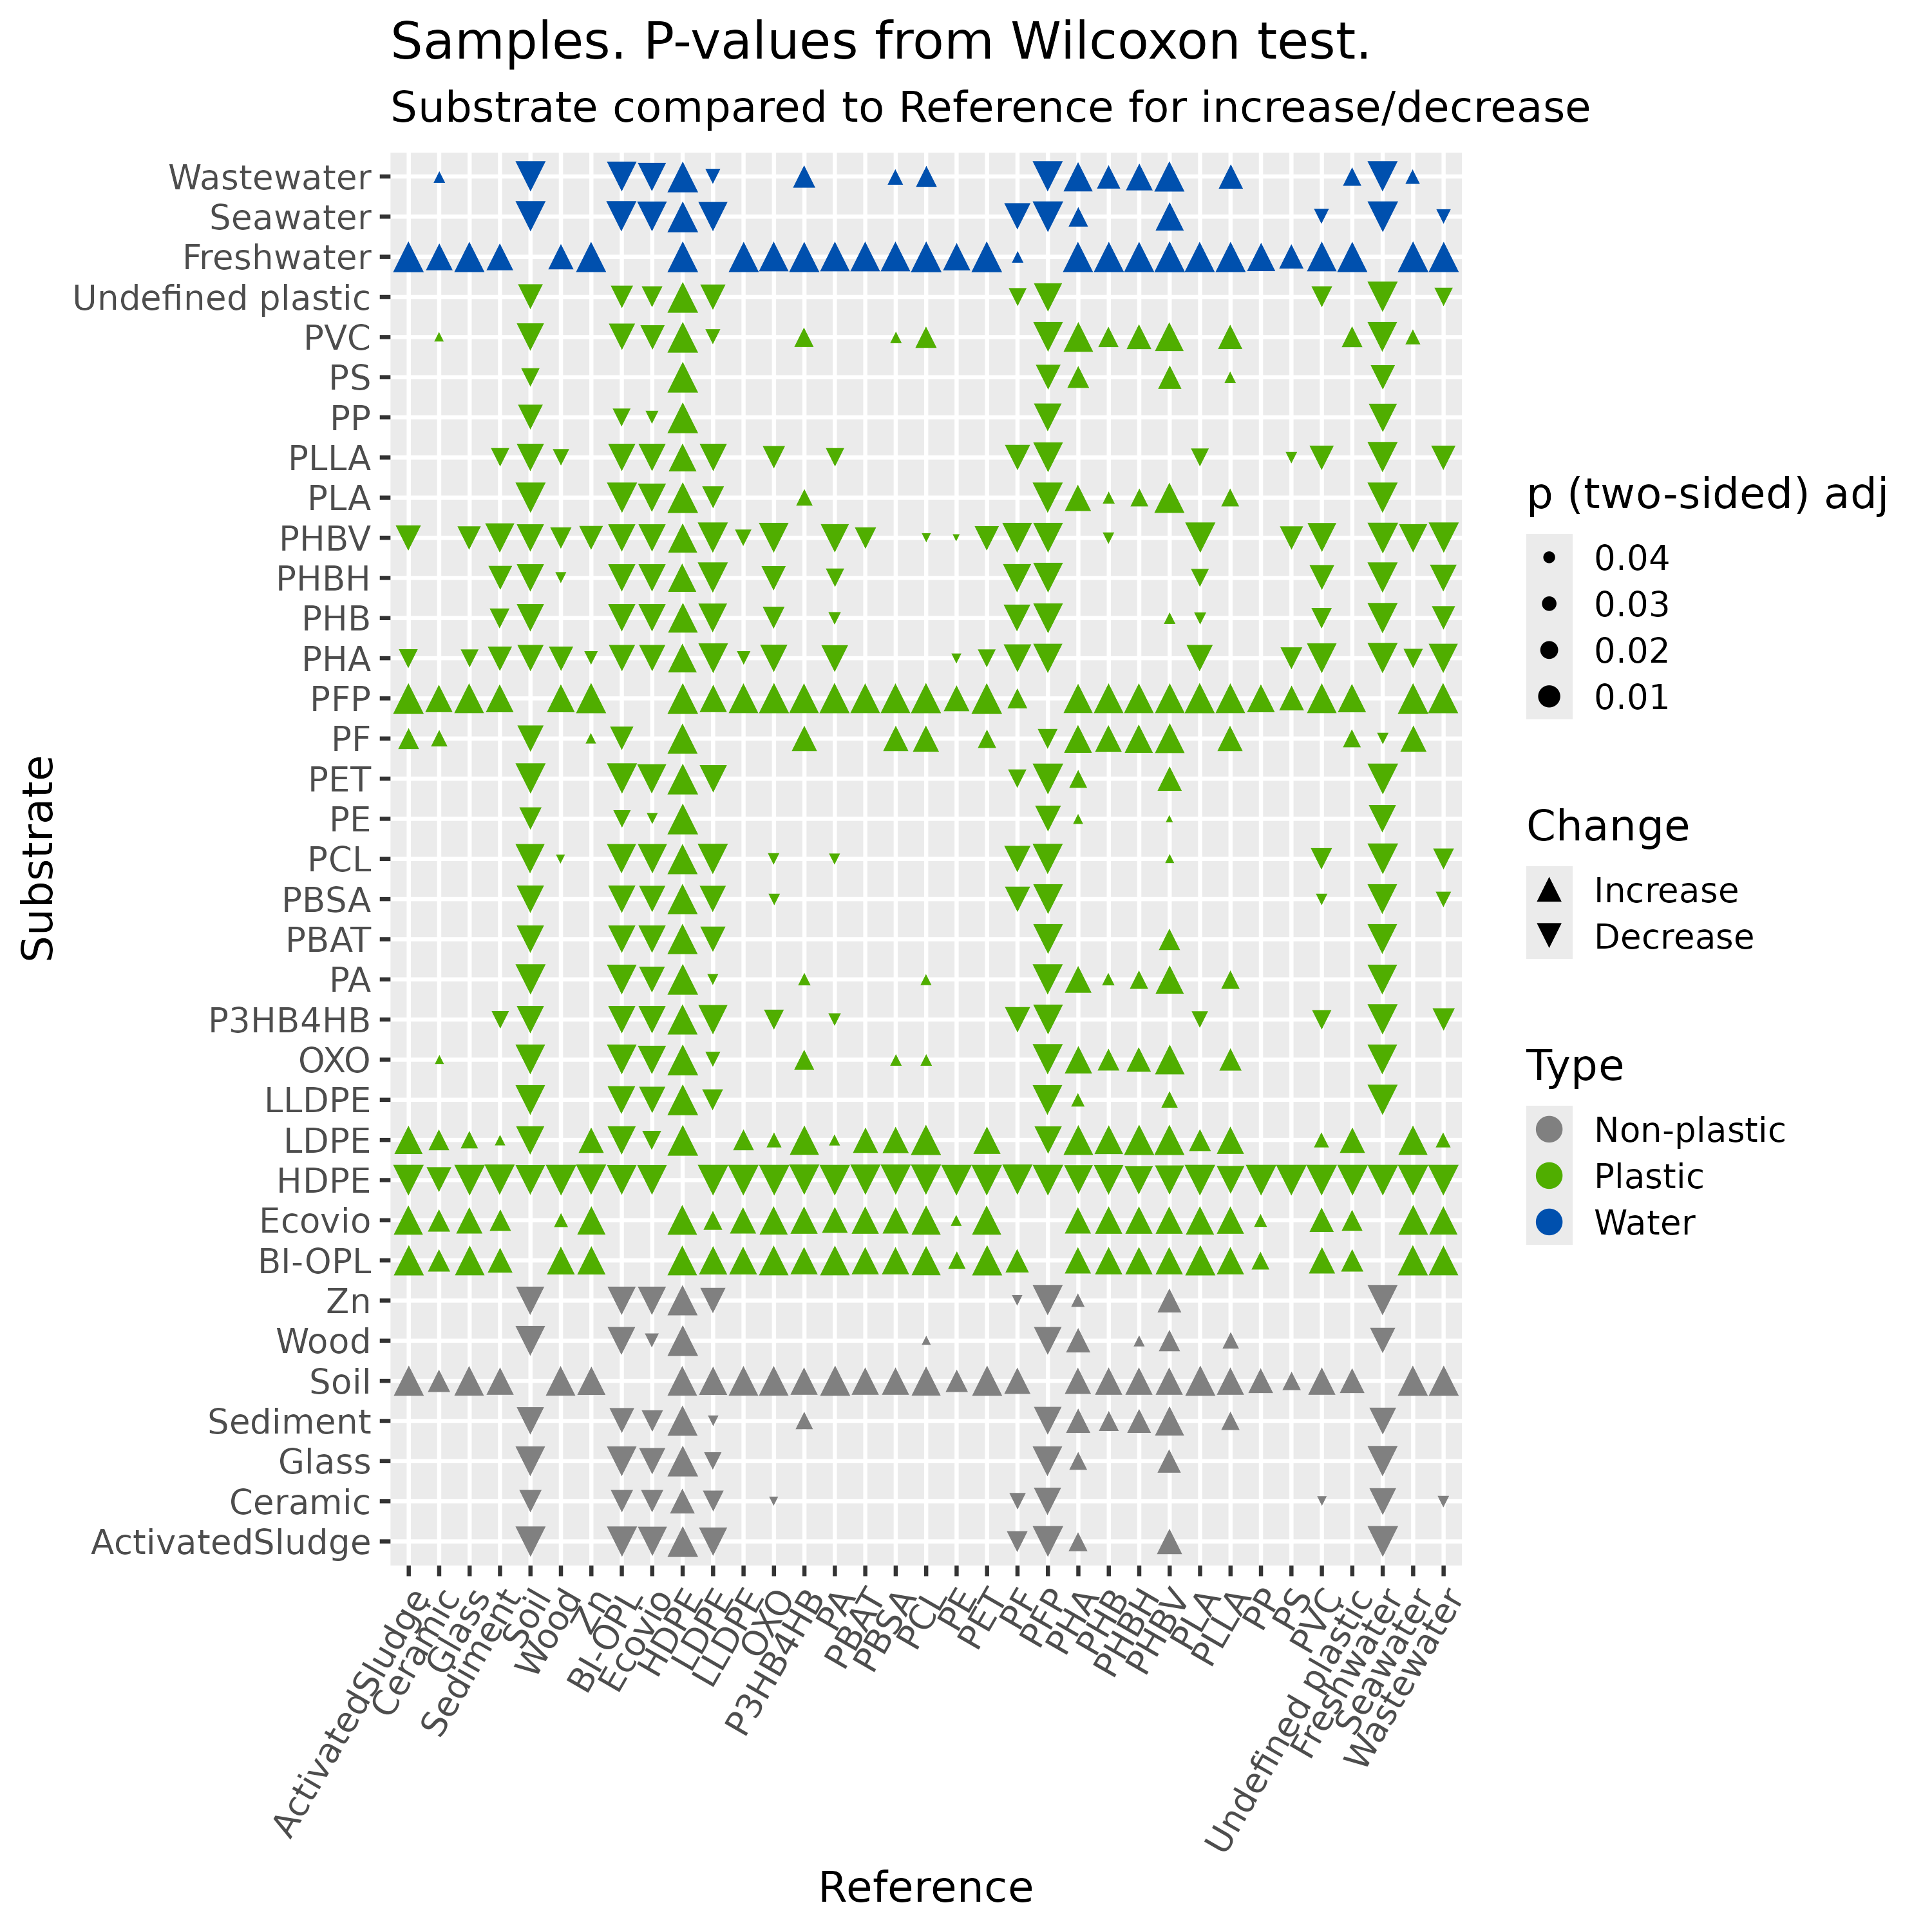
\includegraphics[width = 0.7\textwidth]{figure/wilcox_samples_substrates.png}
    \caption{Wilcoxon Samples Substrate Full}
    \label{wilcox_samples_substrates_full}
\end{figure}


\subsection{Across Mutations}
Figure \ref{mean_genes_sampletype} show the result if instead of the mean mutation percentage for each sample was calculated, the mean mutation percentage per mutation, grouped by sampletype was calculated. \todo{i.e. mutation A12D parC for water: 10\%, A12D parC for plastic: 0\%, A12D parC for non-plastic: 3\%} 

The resulting figure is hard to interpret since many of the genes will have a mean close to zero. If instead a log-scale was used, it removes many of the data points from the water and nonplastic groups, since they have a mean mutation percentage of zero. This skews the figure shown, and end up showing the reverse change as described below. \todo{Since we cannot use the log plot, do we need to use the bad plot instead, or can we skip it and just use stats?}
The mean mutation percentage was significantly different and higher for the plastic samples compared to both the water samples and the non-plastic samples. There is not a significant change between the water group and the non-plastic group.
% There is a significant difference between the different sample types, where plastic show an increase compared to both the water samples and the non-plastic samples.
\todo{n.s. not shown. Why ggsignif show *** when code says n.s.? Both use wilcox.test, and all the other plots give the same result? Manually removed for now.}

\begin{figure}[h]
    \centering
    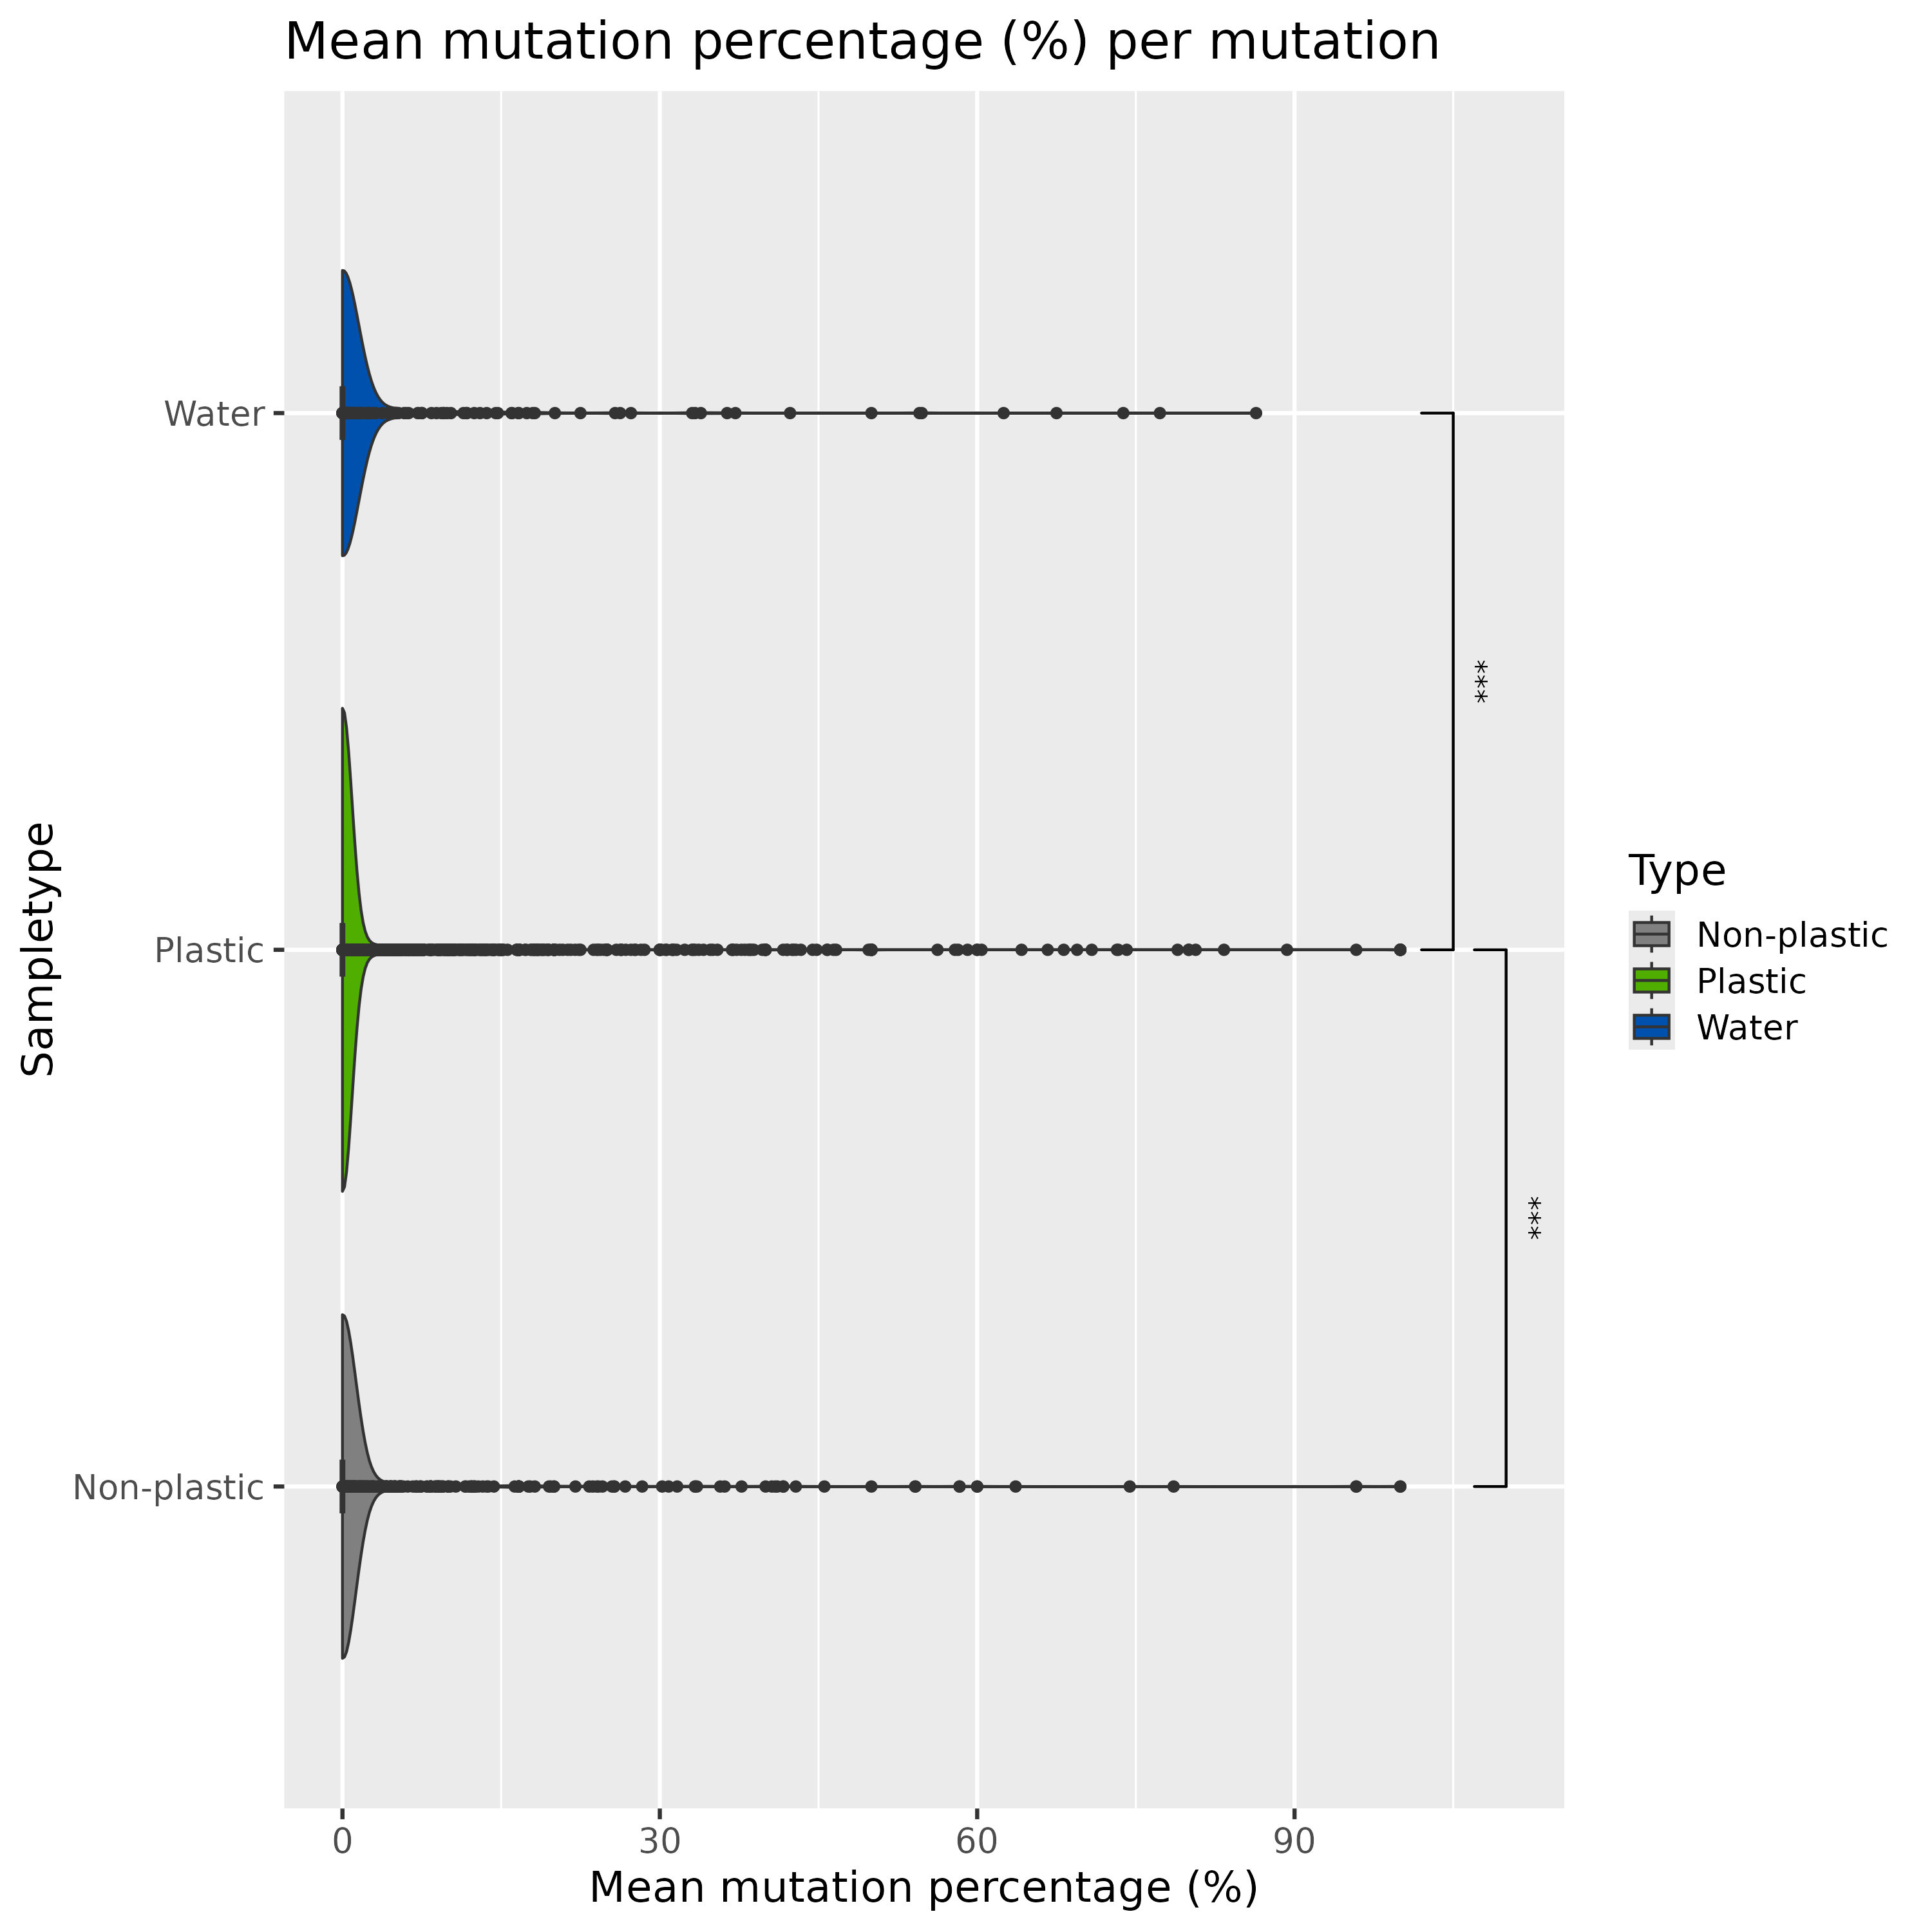
\includegraphics[width = 0.7\textwidth]{figure/mean_genes_sampletype.png}
    \caption{Mean mutations Sampletype}
    \label{mean_genes_sampletype}
\end{figure}

Figure \ref{mean_genes_substrate} show the mean mutation percentage per mutation grouped by substrate type. The figure shows that there are differences between the different substrates, and this is supported by figure \ref{wilcox_genes_substrate} which show the p-values from a Wilcoxon test between them, and that there are significant differences between many of them.
% Since figure \ref{mean_genes_substrate} uses a log-scale for visibility, the normal interpretation of the box-plot cannot be done since many points are erroneously removed, and therefore is only for visualizing the mutation rate.
The substrates which have the highest mean mutation percentage are PFP, PE, Ecovio, and BI-OPL from the plastic group as well as soil and wood from the non-plastic sampletypes. Freshwater had a significant increase to most other substrates.

% FROM samples substrates: 
% In figure \ref{mean_samples_substrate} the samples are instead grouped by substrate type, which show that there are differences for different plastics, as well as other substrates. Figure \ref{wilcox_samples_substrate} show the statistical significance of the comparison, when a wilcoxon test was done for the Substrate versus the Reference, as well as if there is an increase of the pseudo-mean compared to the reference. Note that all comparisons were done, but only the significant ones (p < 0.05) are shown. It is shown that there are some plastics that has a significant higher mean mutation percentage than most other substrates. These include PFP, LDPE, Ecovio and BI-OPL. The last two plastics are biodegradable plastics. The plastic substrates that has a significant higher mean mutation percentage than seawater or wastewater include PVC and PF in addition to the other plastics mentioned before. There are also some plastics which have significantly different lower mean mutation percentage than almost all other substrates, the most notable of which is high-density polyethylene (HDPE), poly(3-hydroxybutyrate-co-3-hydroxyvalerate) (PHBV) and polyhydroxyalkanoate (PHA), of which the latter two are biodegradable polymers while the first one is not. Almost all substrates has a significantly different lower mean mutation percentage than the freshwater samples, the exception of which is leaf, rock, Ecovio, BI-OPL, and PFP where there is no significant difference. The soil samples also has a significant higher mean mutation percentage compared to many other substrates.

\begin{figure}[h]
    \centering
    \subfloat[This plot also weird. If we add pseudocount, then we get box to the left and outliers to the right? Don't know if it is better, but at least visible?\label{mean_genes_substrate}]{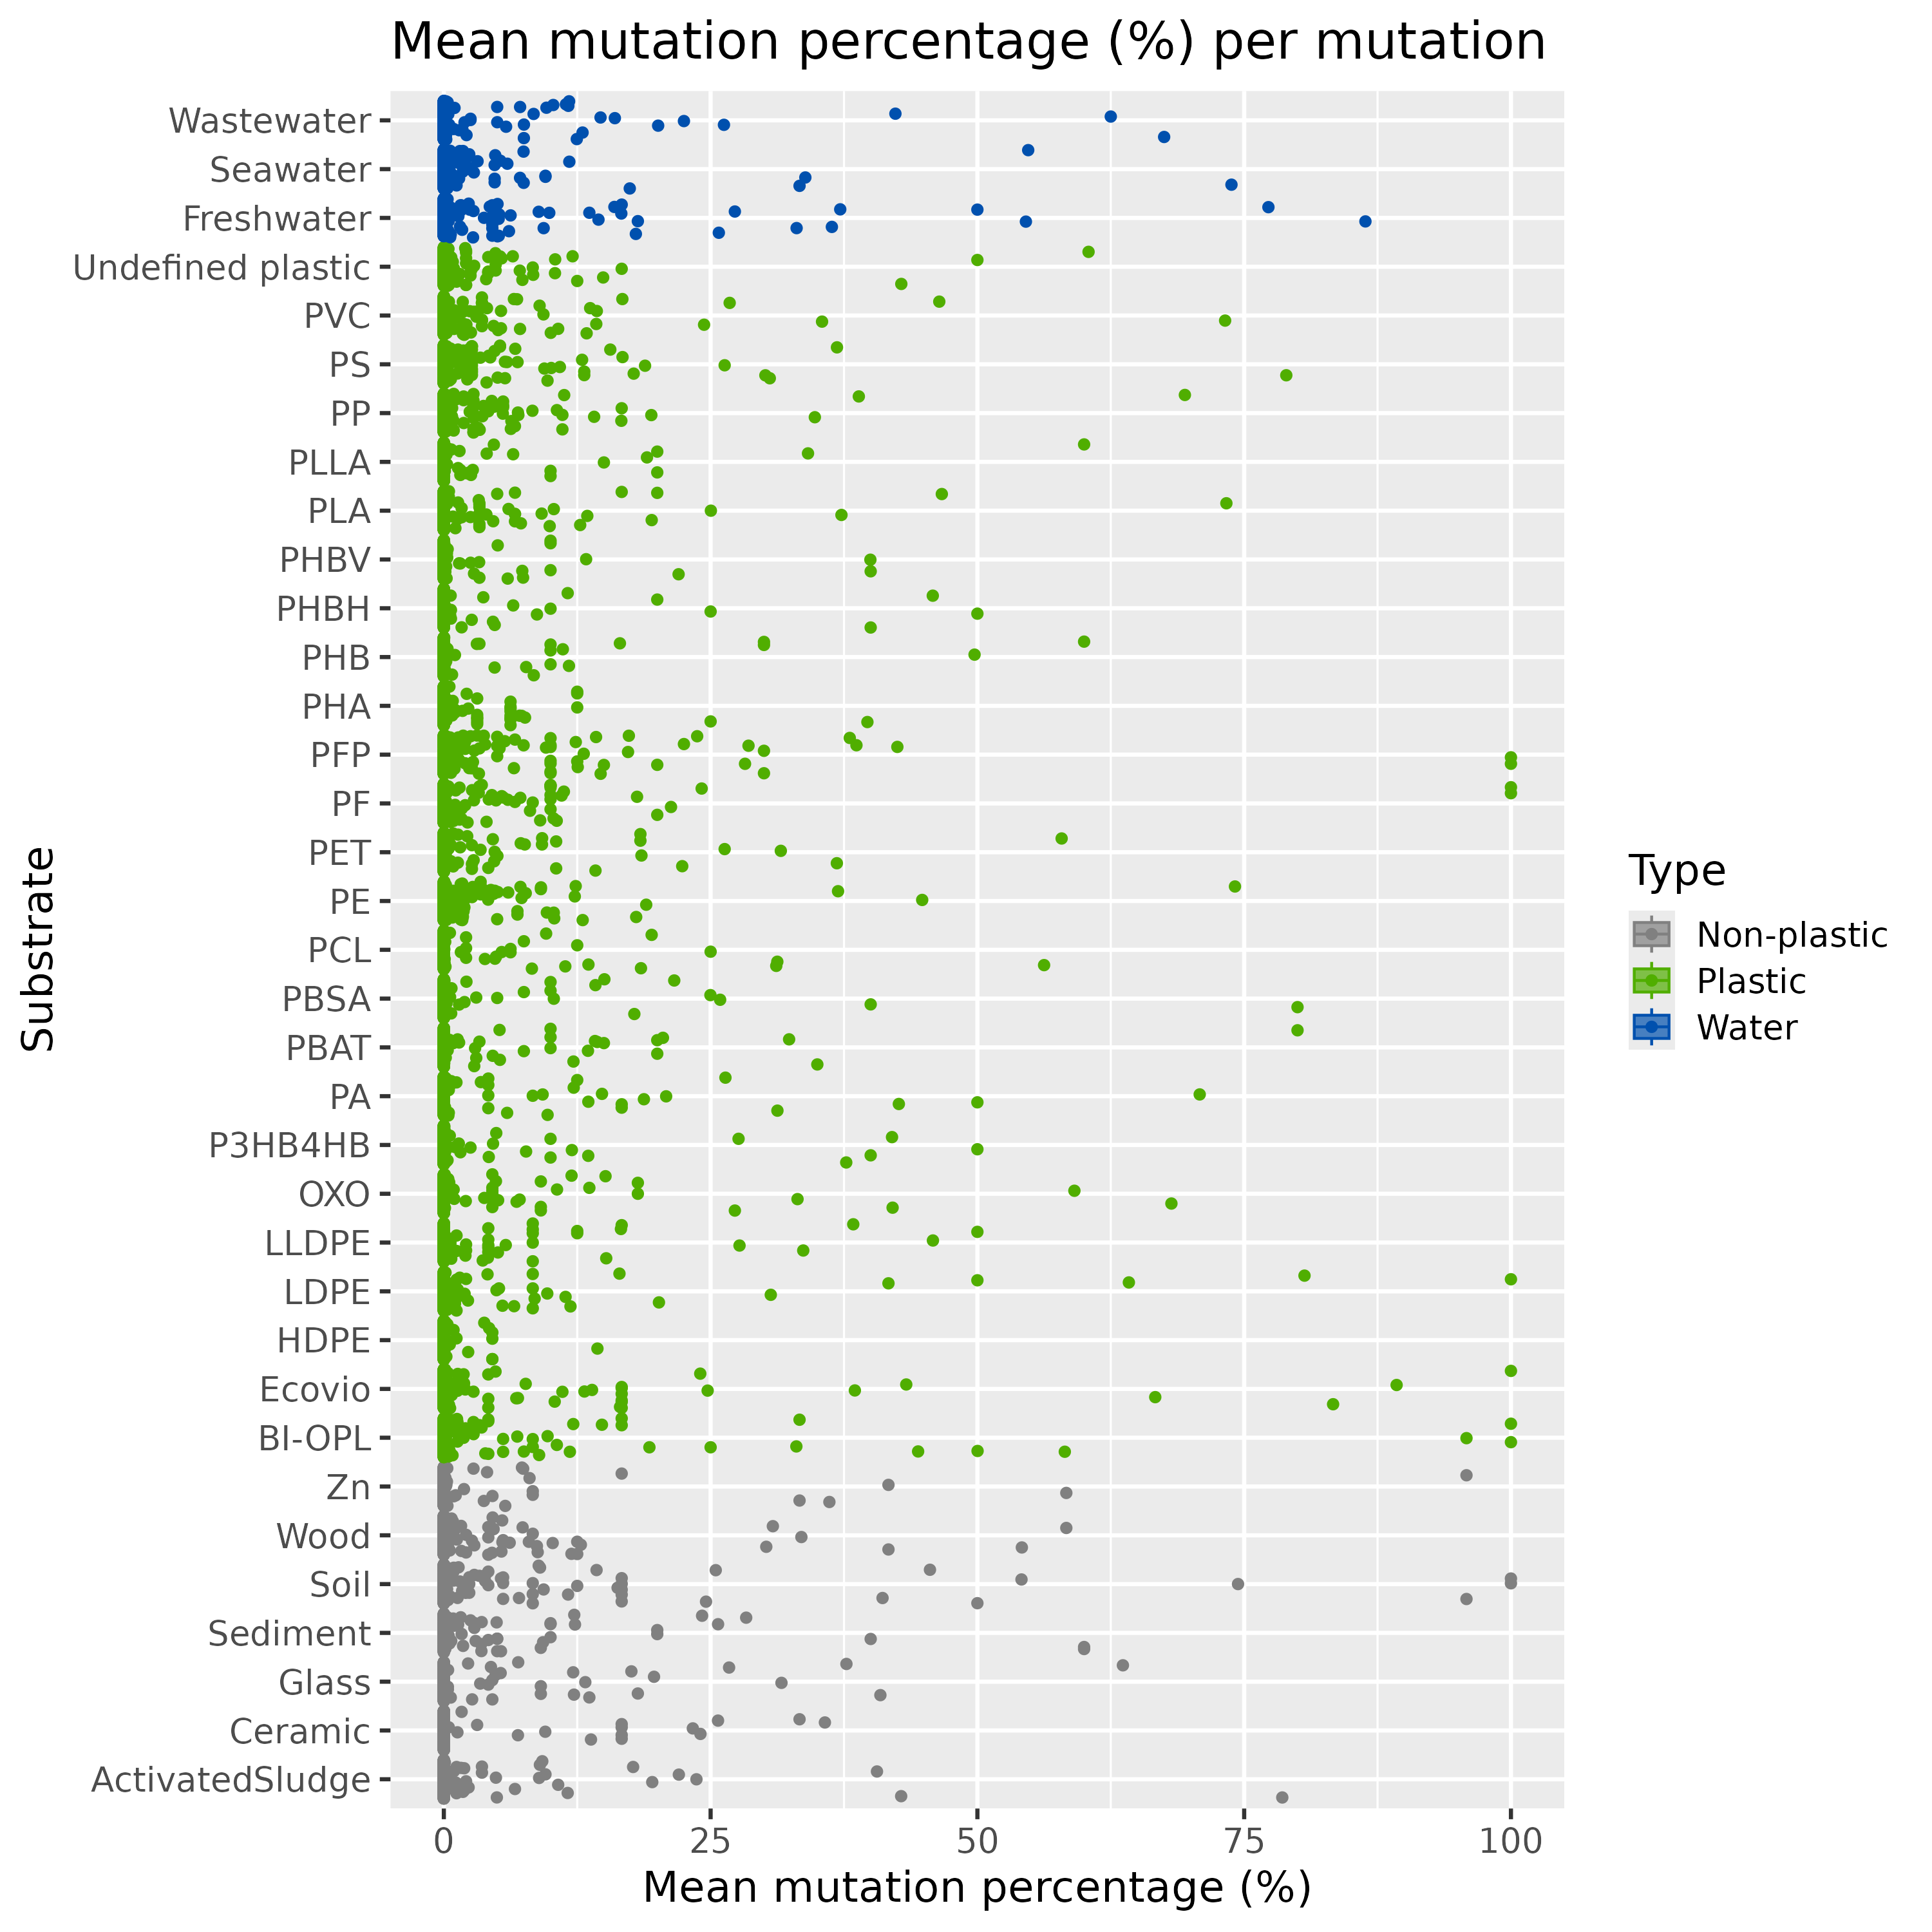
\includegraphics[width=0.5\textwidth]{figure/mean_genes_substrate.png}} 
    \subfloat[caption2.\label{wilcox_genes_substrate}]{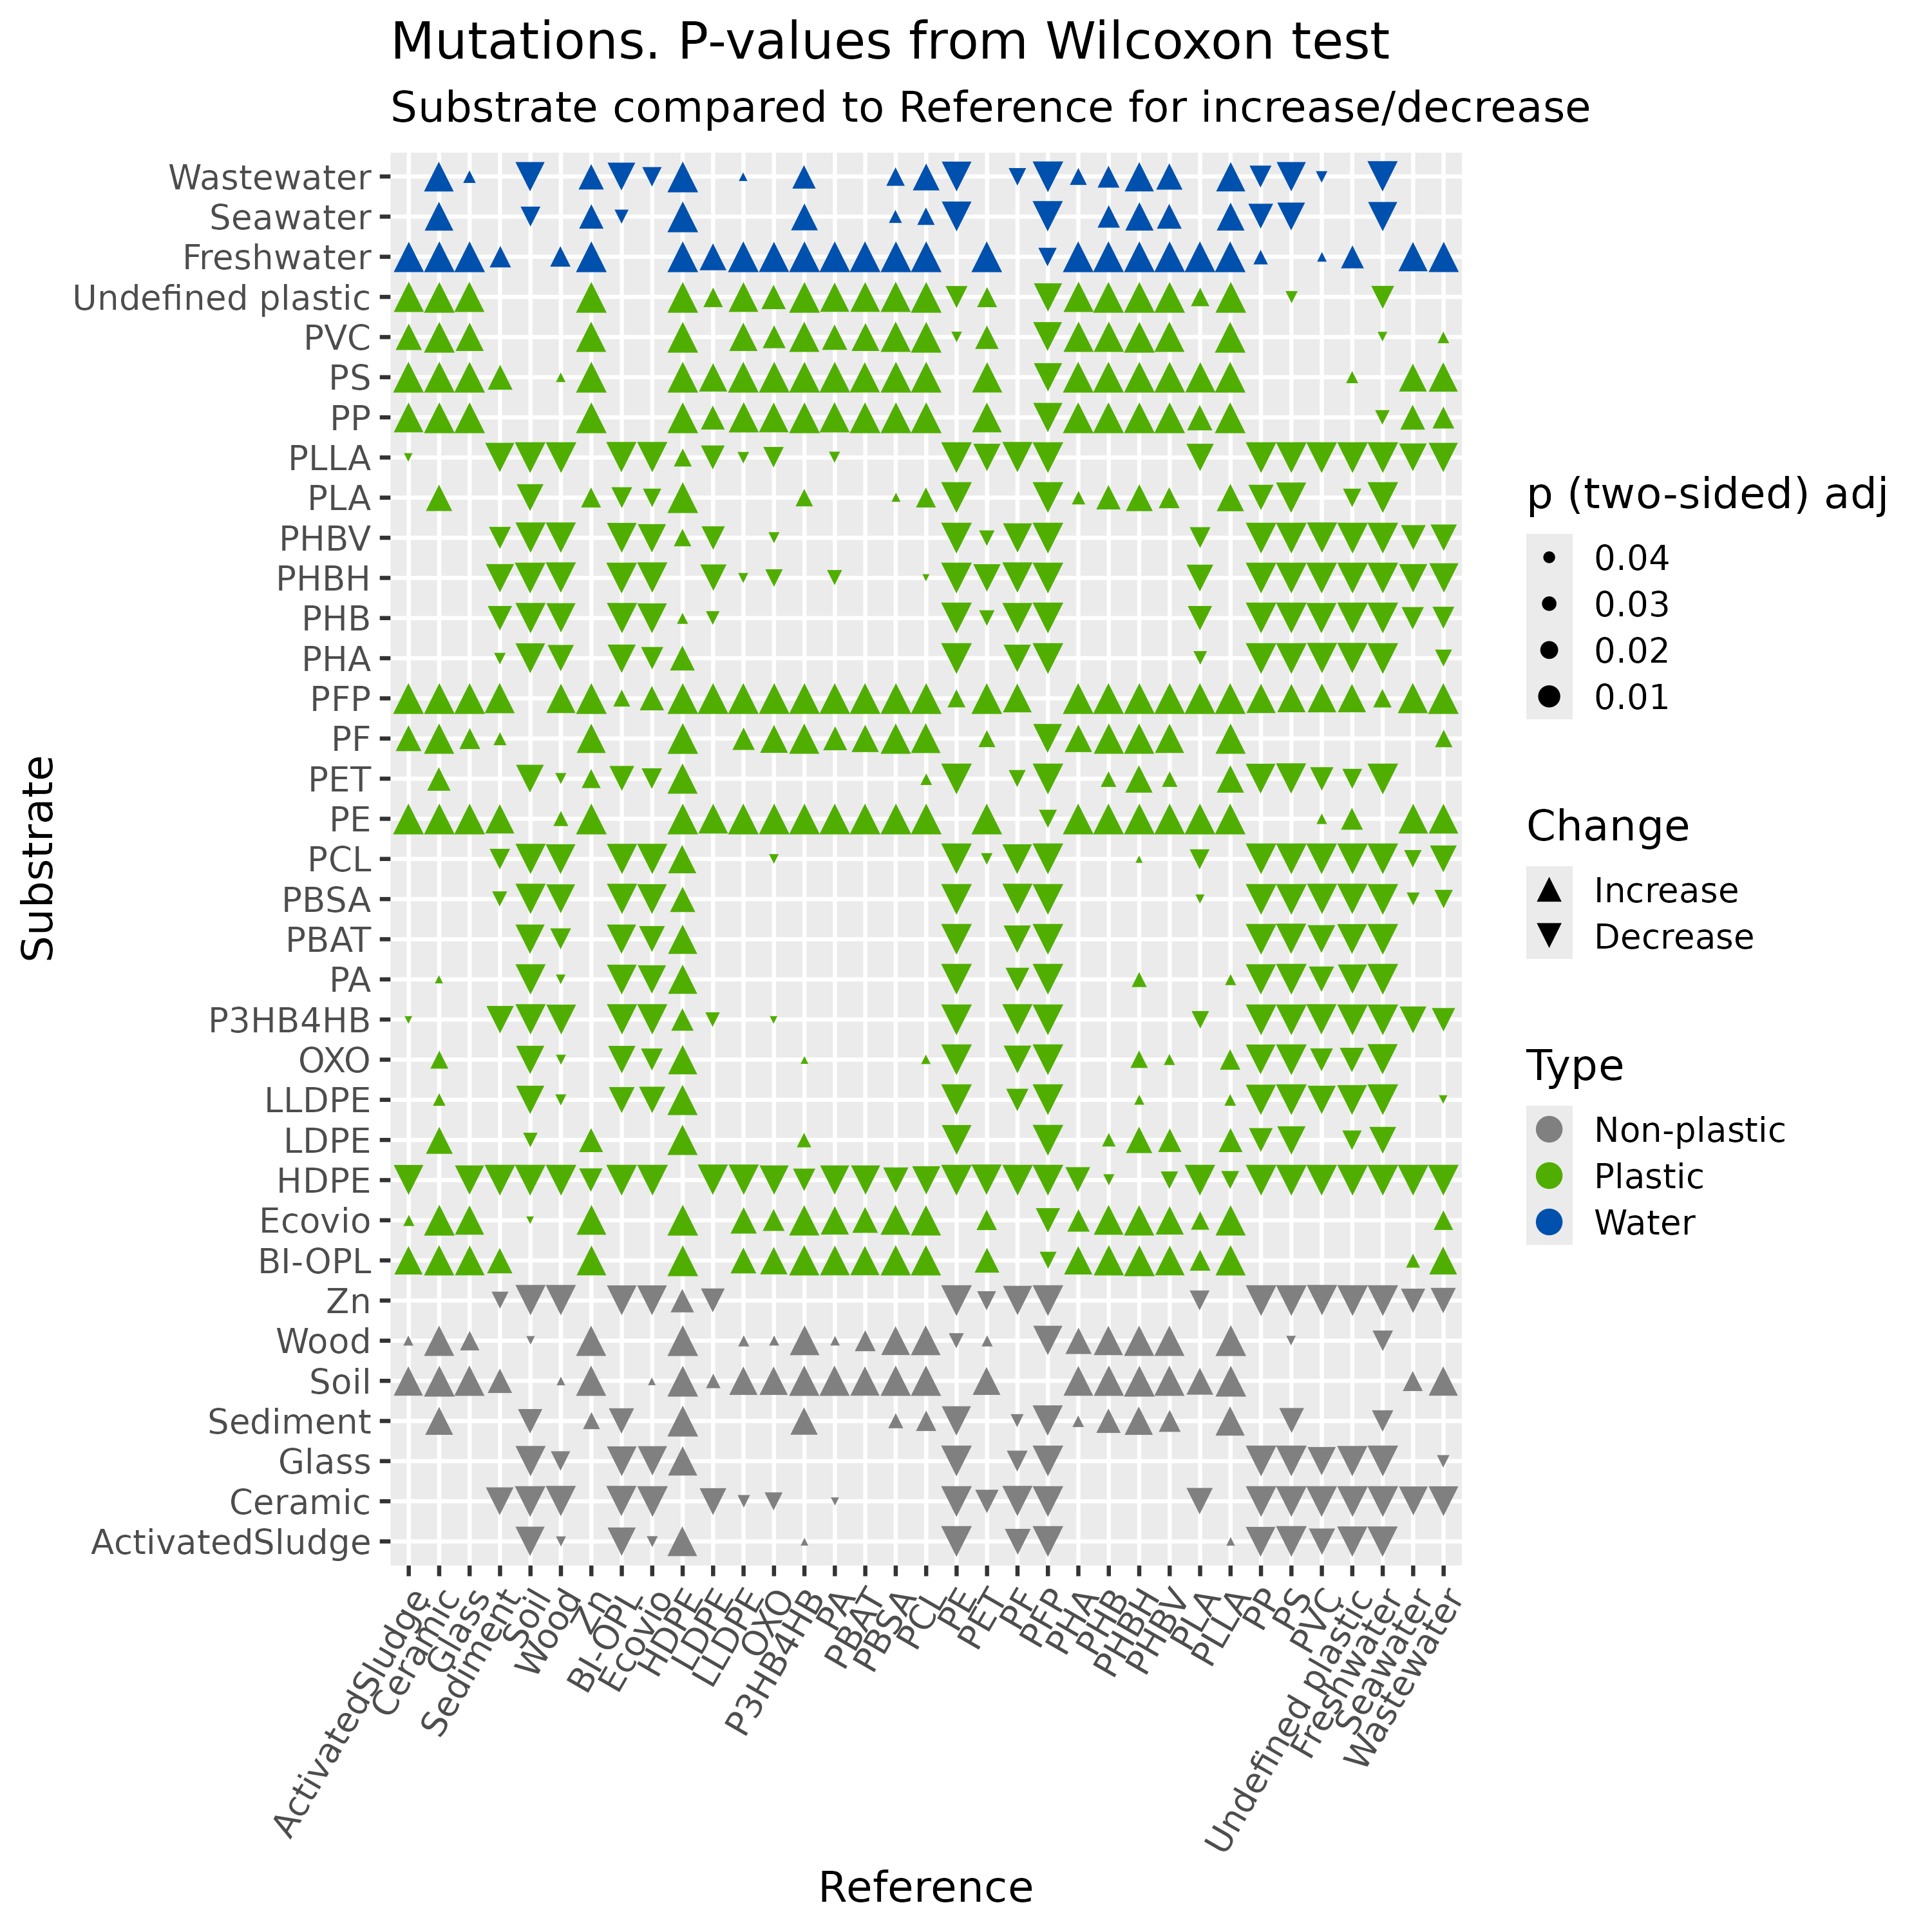
\includegraphics[width=0.5\textwidth]{figure/wilcox_genes_substrates.png}}
    \caption{Mean genes substrate.}
    \label{both_mean_genes_substrate}
\end{figure}

Figure \ref{pointplot_mutations} show the mean mutation percentage for different genes in varying substrates. Only mutations with a mean mutation percentage higher than 25 percent are included in the figure. 
The figure shows that there are certain mutations which occur in most substrates and some that only ooccur in some substrates. The ones which occur in almost all samples are Q1073R in rpoB which confer resistance to rifampicin, G1245B in gyrB which confer resistance to aminocoumarin, and D244Y in rpoC which confer resistance to vancomycin.

\begin{figure}[h]
    \centering
    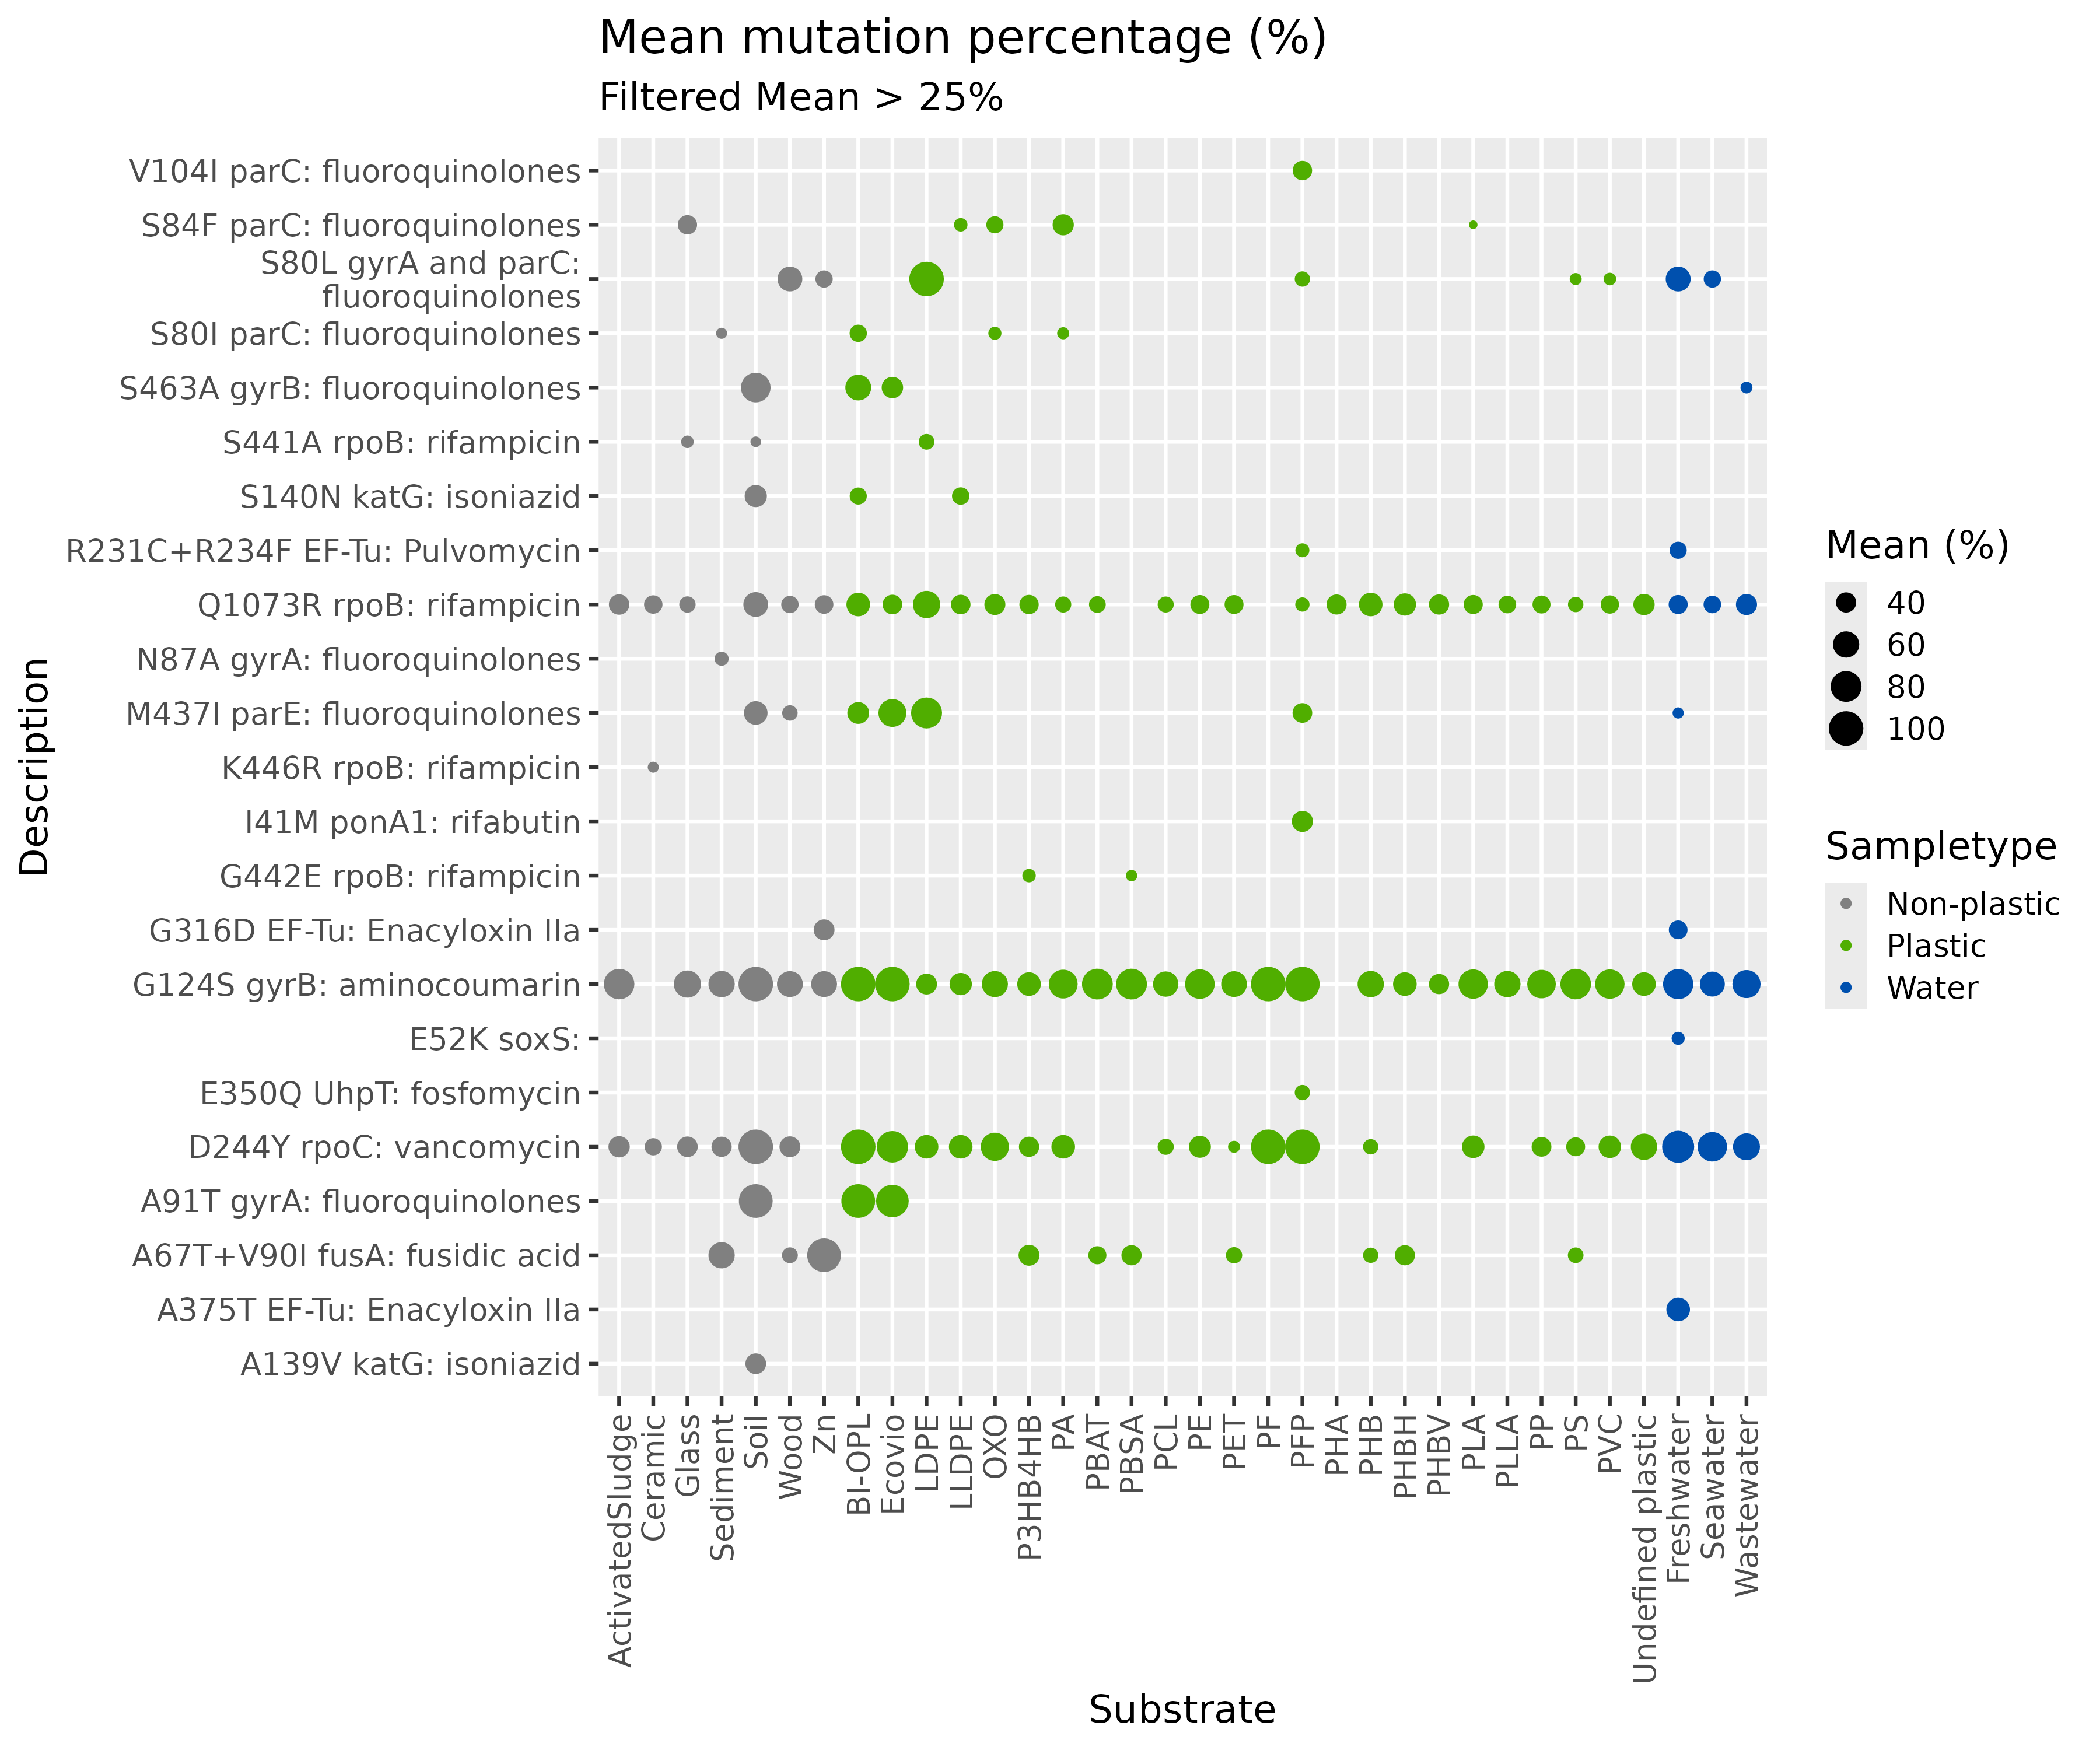
\includegraphics[width = \textwidth]{figure/relative_mean_points_25.png}
    \caption{Filtered mean mutation percentage per mutation. TODO: include this or skip? Filter to exclude those with < 3 samples?}
    \label{pointplot_mutations}
\end{figure}


\section{Random Forest}
% Removed:
% D87H:Pseudomonas aeruginosa gyrA: fluoroquinolones
% D87H:Burkholderia dolosa gyrA: fluoroquinolones
%
% Renamed: There is one AMR Gene Family which has a very long name:
% "ATP-binding cassette (ABC) antibiotic efflux pump;General Bacterial Porin with reduced permeability to beta-lactams;major facilitator superfamily (MFS) antibiotic efflux pump;resistance-nodulation-cell division (RND) antibiotic efflux pump"
In the following figures only the ten most significant AMR Gene Families or mutations are shown. However, there are in all cases several more which are not shown. Figures showing all of the significant variables can be found in the Jupyter Notebook.\todo{Not sure if \emph{all} of them can be shown, but at least 50 is possible in a really long plot} 

\subsection{AMR Gene Family}
\subsubsection{Sampletypes}
Figure \ref{amr_sampletype_bar_10} show the mean decrease in Gini impurity for five different AMR Gene Families, which was found to be significant.
%todo{true or not? true since kruskal-wallace test found X taxa singificant} when the samples are grouped by sampletype.
Three of the families may be used to identify the non-plastic samples, which include fluoroquinolone resistant parC and gyrA as well as daptomycin-resistant beta-subunit of RNA polymerase (rpoB). 
The two significant gene families for the water samples were vancomycin-resistant beta prime subunit of RNA polymerase (rpoC) and rifampicin-reistant rpoC. 
However, note the negative sign of these which indicate that these AMR Gene Families are more important to determine that a sample is in the reference group (the other groups) than in the water group. 
\todo{It is significant, shows that a samples is NOT in the water group. As mentioned above. Can only say that a sample is from the non-plastic group, or NOT in the water group, not the abundance of it.}

If instead the samples are grouped by substrate type, as shown in figure \ref{amr_substrate_bar}, there are a lot more AMR Gene Families which distinguishes the samples in one group from another.
The most prevalent substrate in this figure is the activated sludge, which has four different AMR Gene Families that distinguishes it.
The one labelled Multiple Resistant Variants has been renamed from "ATP-binding cassette (ABC) antibiotic efflux pump; General Bacterial Porin with reduced permeability to beta-lactams; major facilitator superfamily (MFS) antibiotic efflux pump; resistance-nodulation-cell division (RND) antibiotic efflux pump". \todo{comment or just observation?}
All Mean Decrease Gini impurity values are positive for this grouping, there are no significant AMR Gene Families which may be used to conclude that a sample is not from a specific substrate as was the case with the sampletypes. 


\begin{figure}[h]
    \centering
    \subfloat[caption1.\label{amr_sampletype_bar_10}]{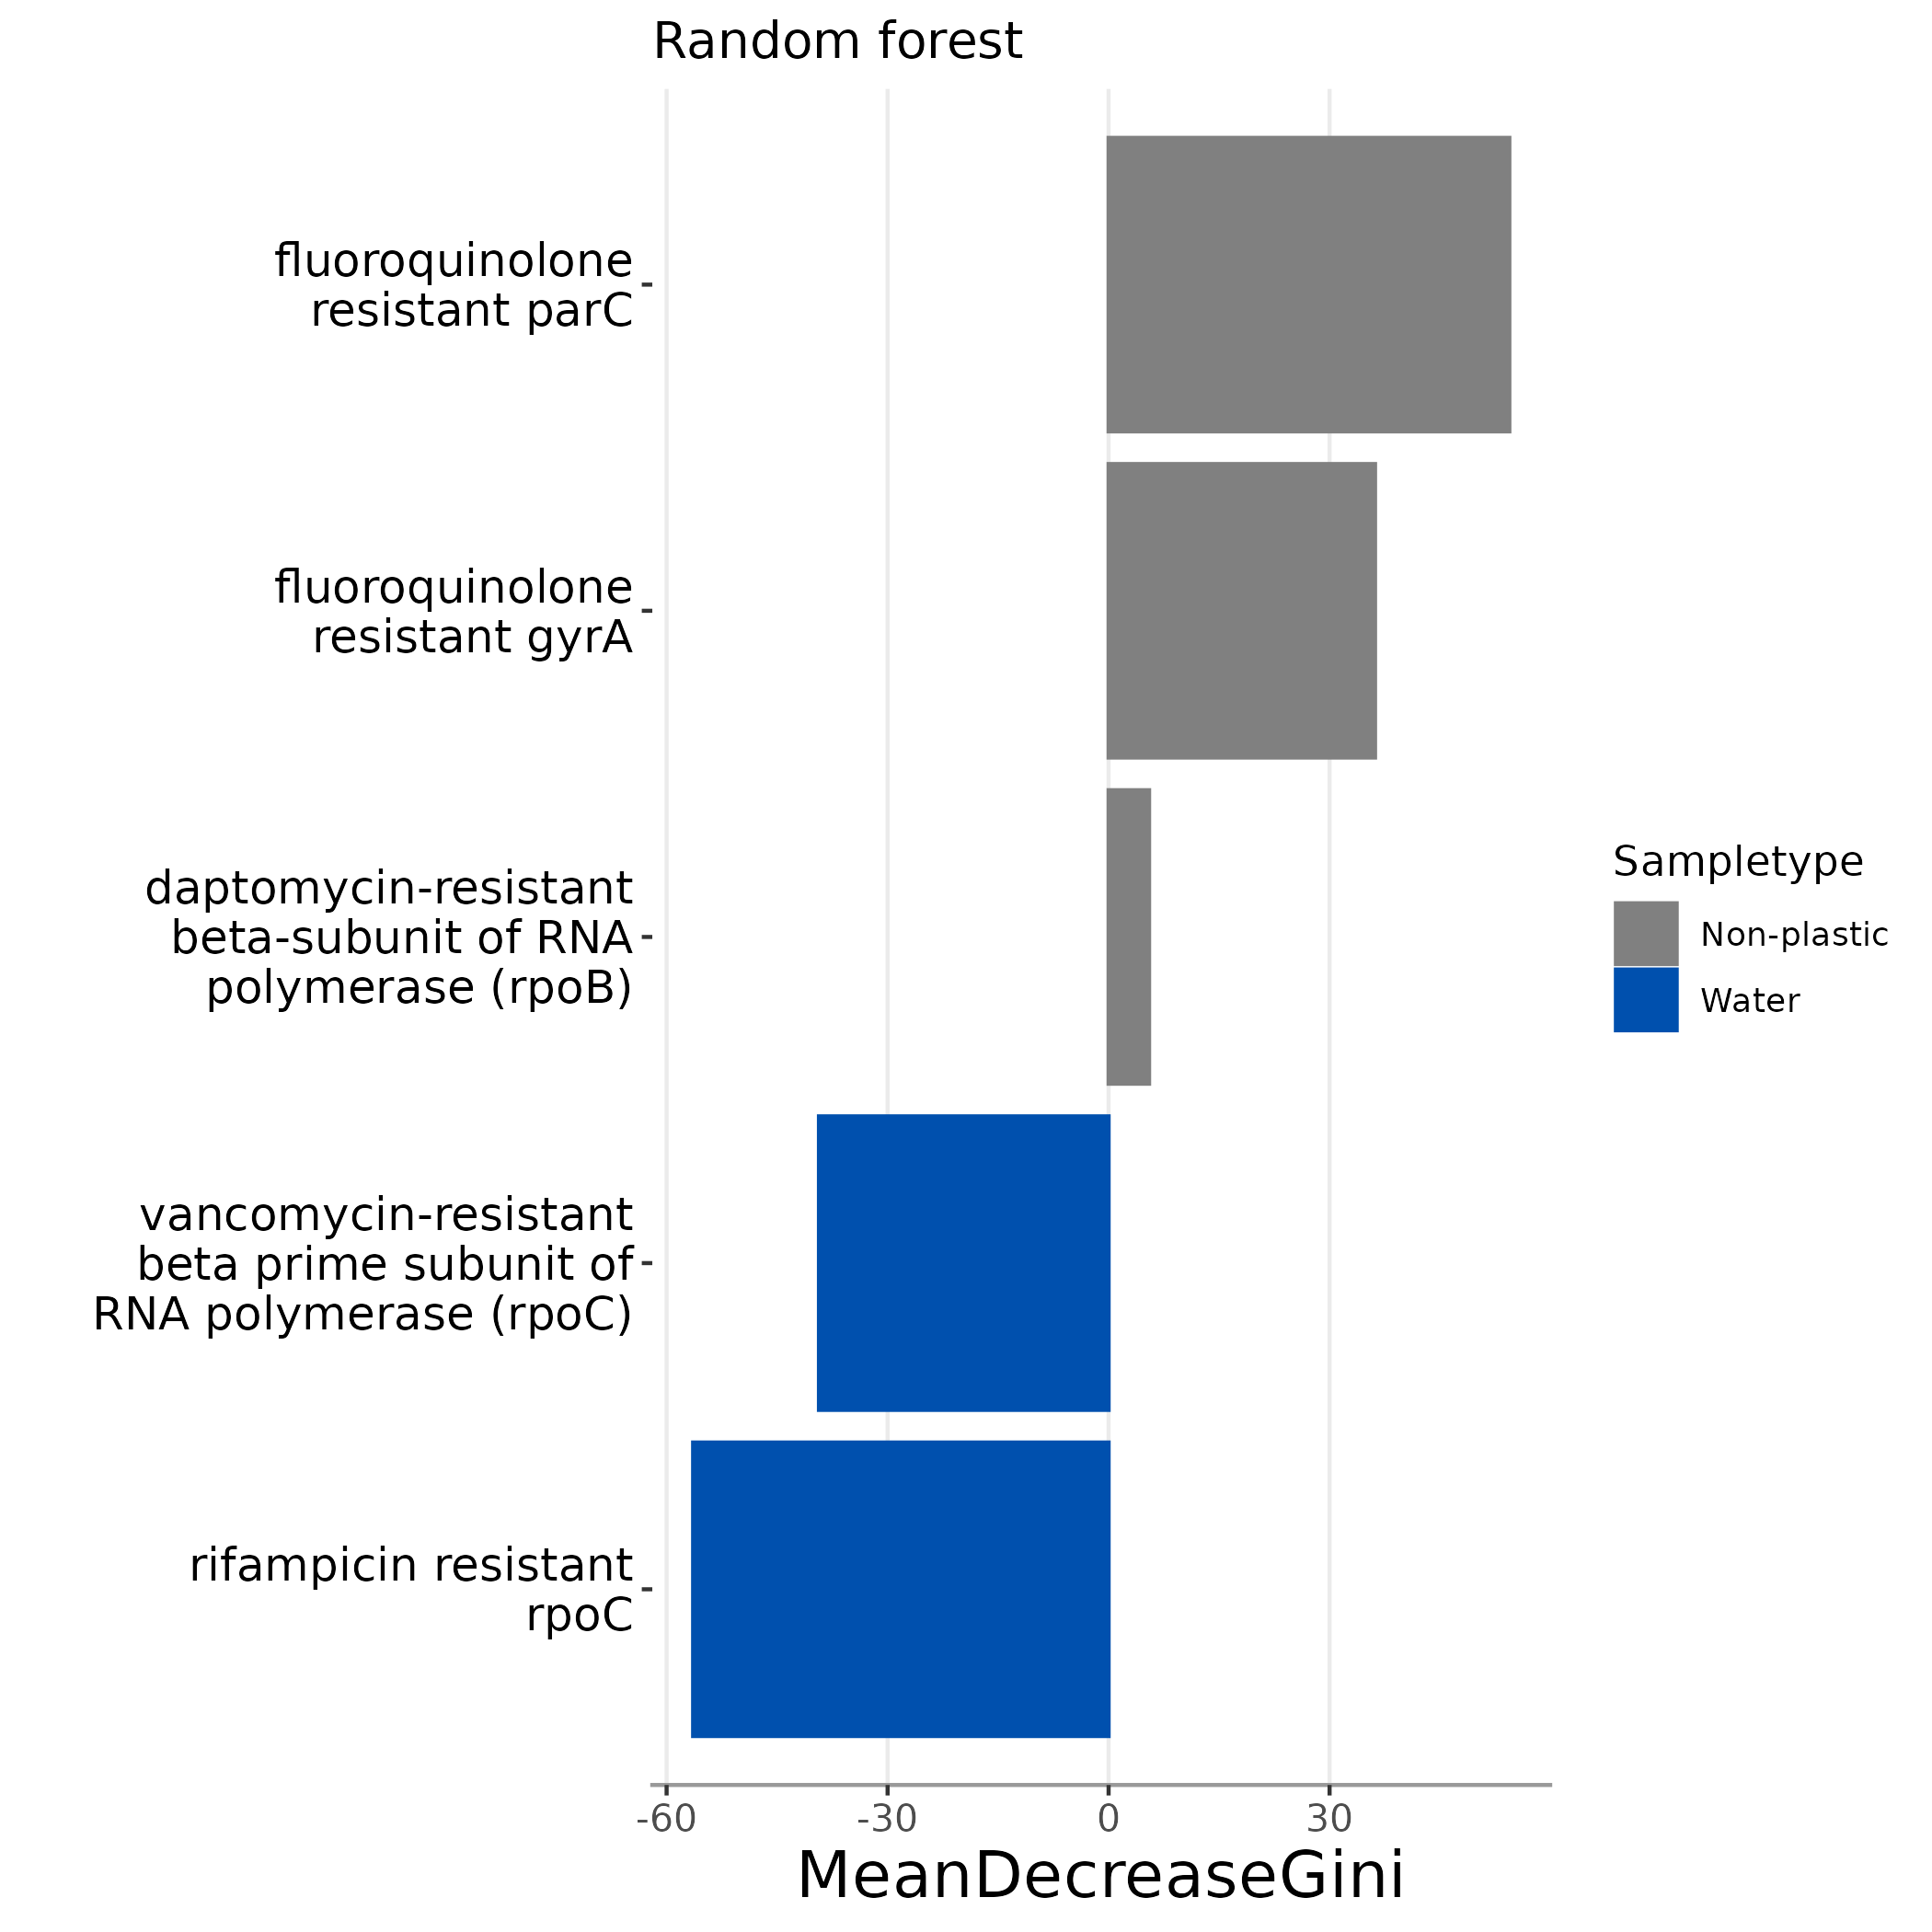
\includegraphics[width=0.5\textwidth]{figure/relative_forest_sampletype_amr_bar.png}}
    \subfloat[caption2.\label{amr_sampletype_abund}]{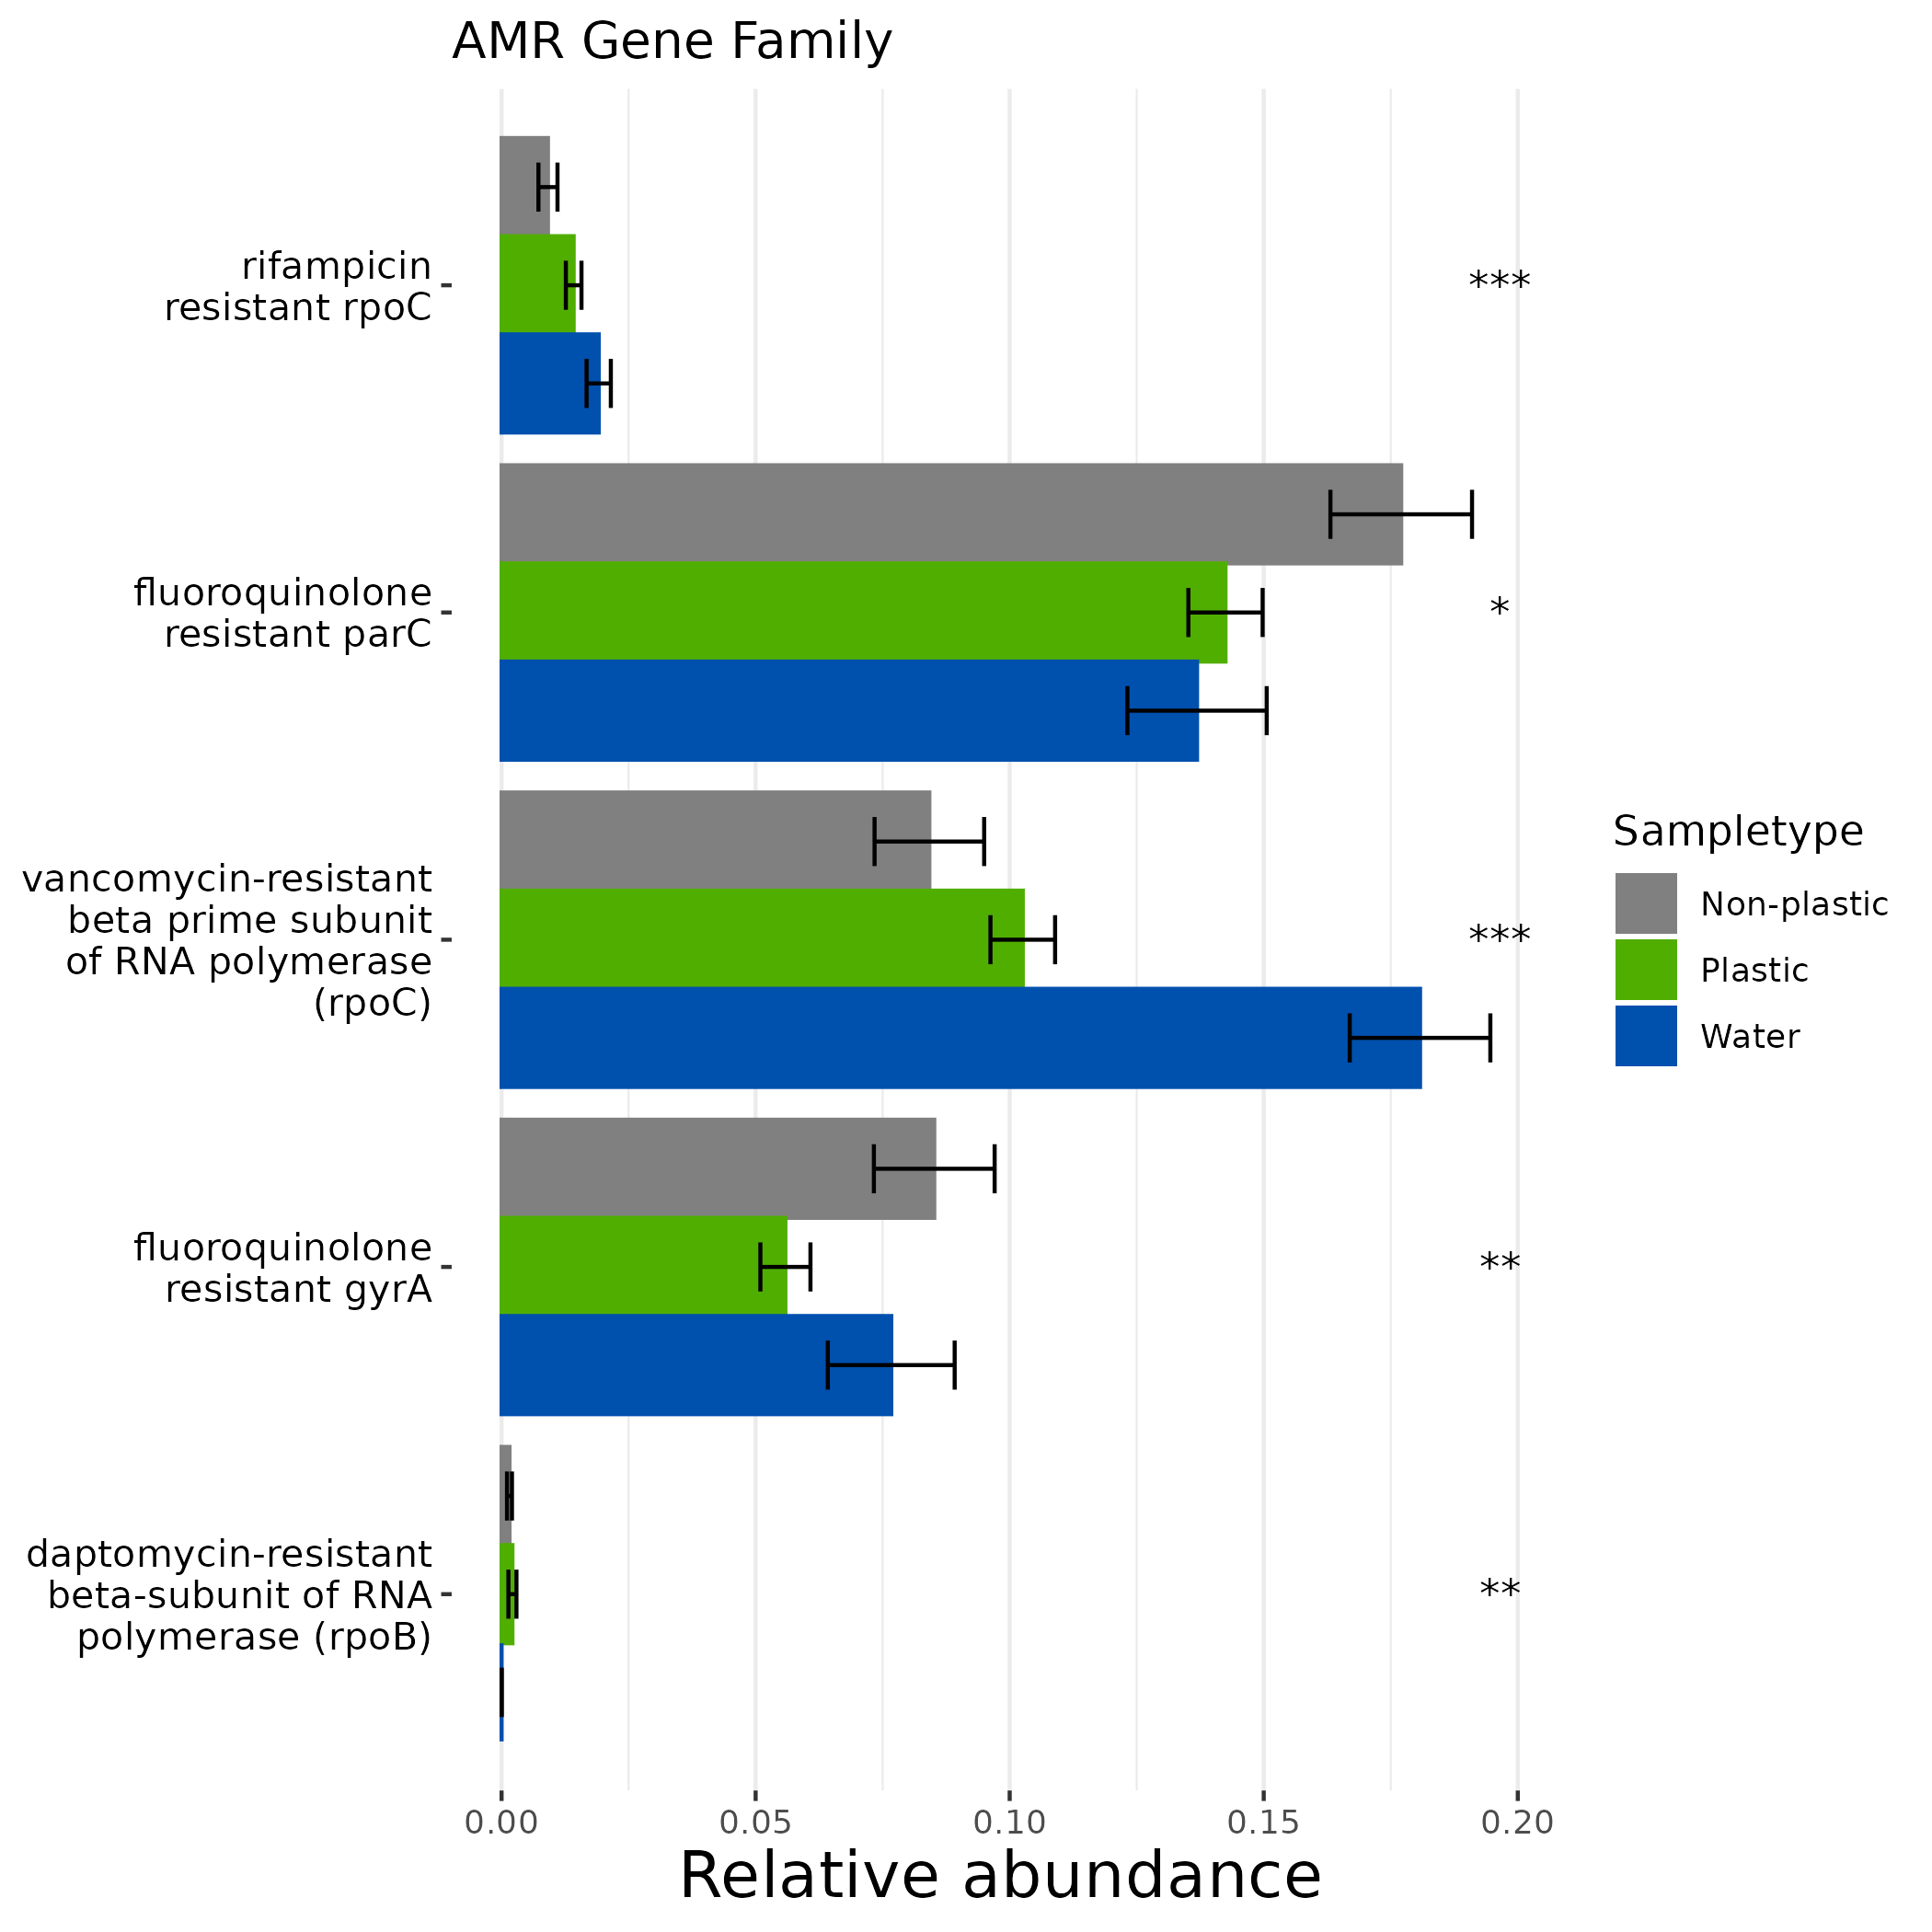
\includegraphics[width=0.5\textwidth]{figure/relative_forest_sampletype_amr_abund.png}}
    \caption{AMR Sampletype}
    \label{amr_sampletype}
\end{figure}

\begin{figure}[h]
    \centering
    \subfloat[Barplot, keep.\label{amr_substrate_bar}]{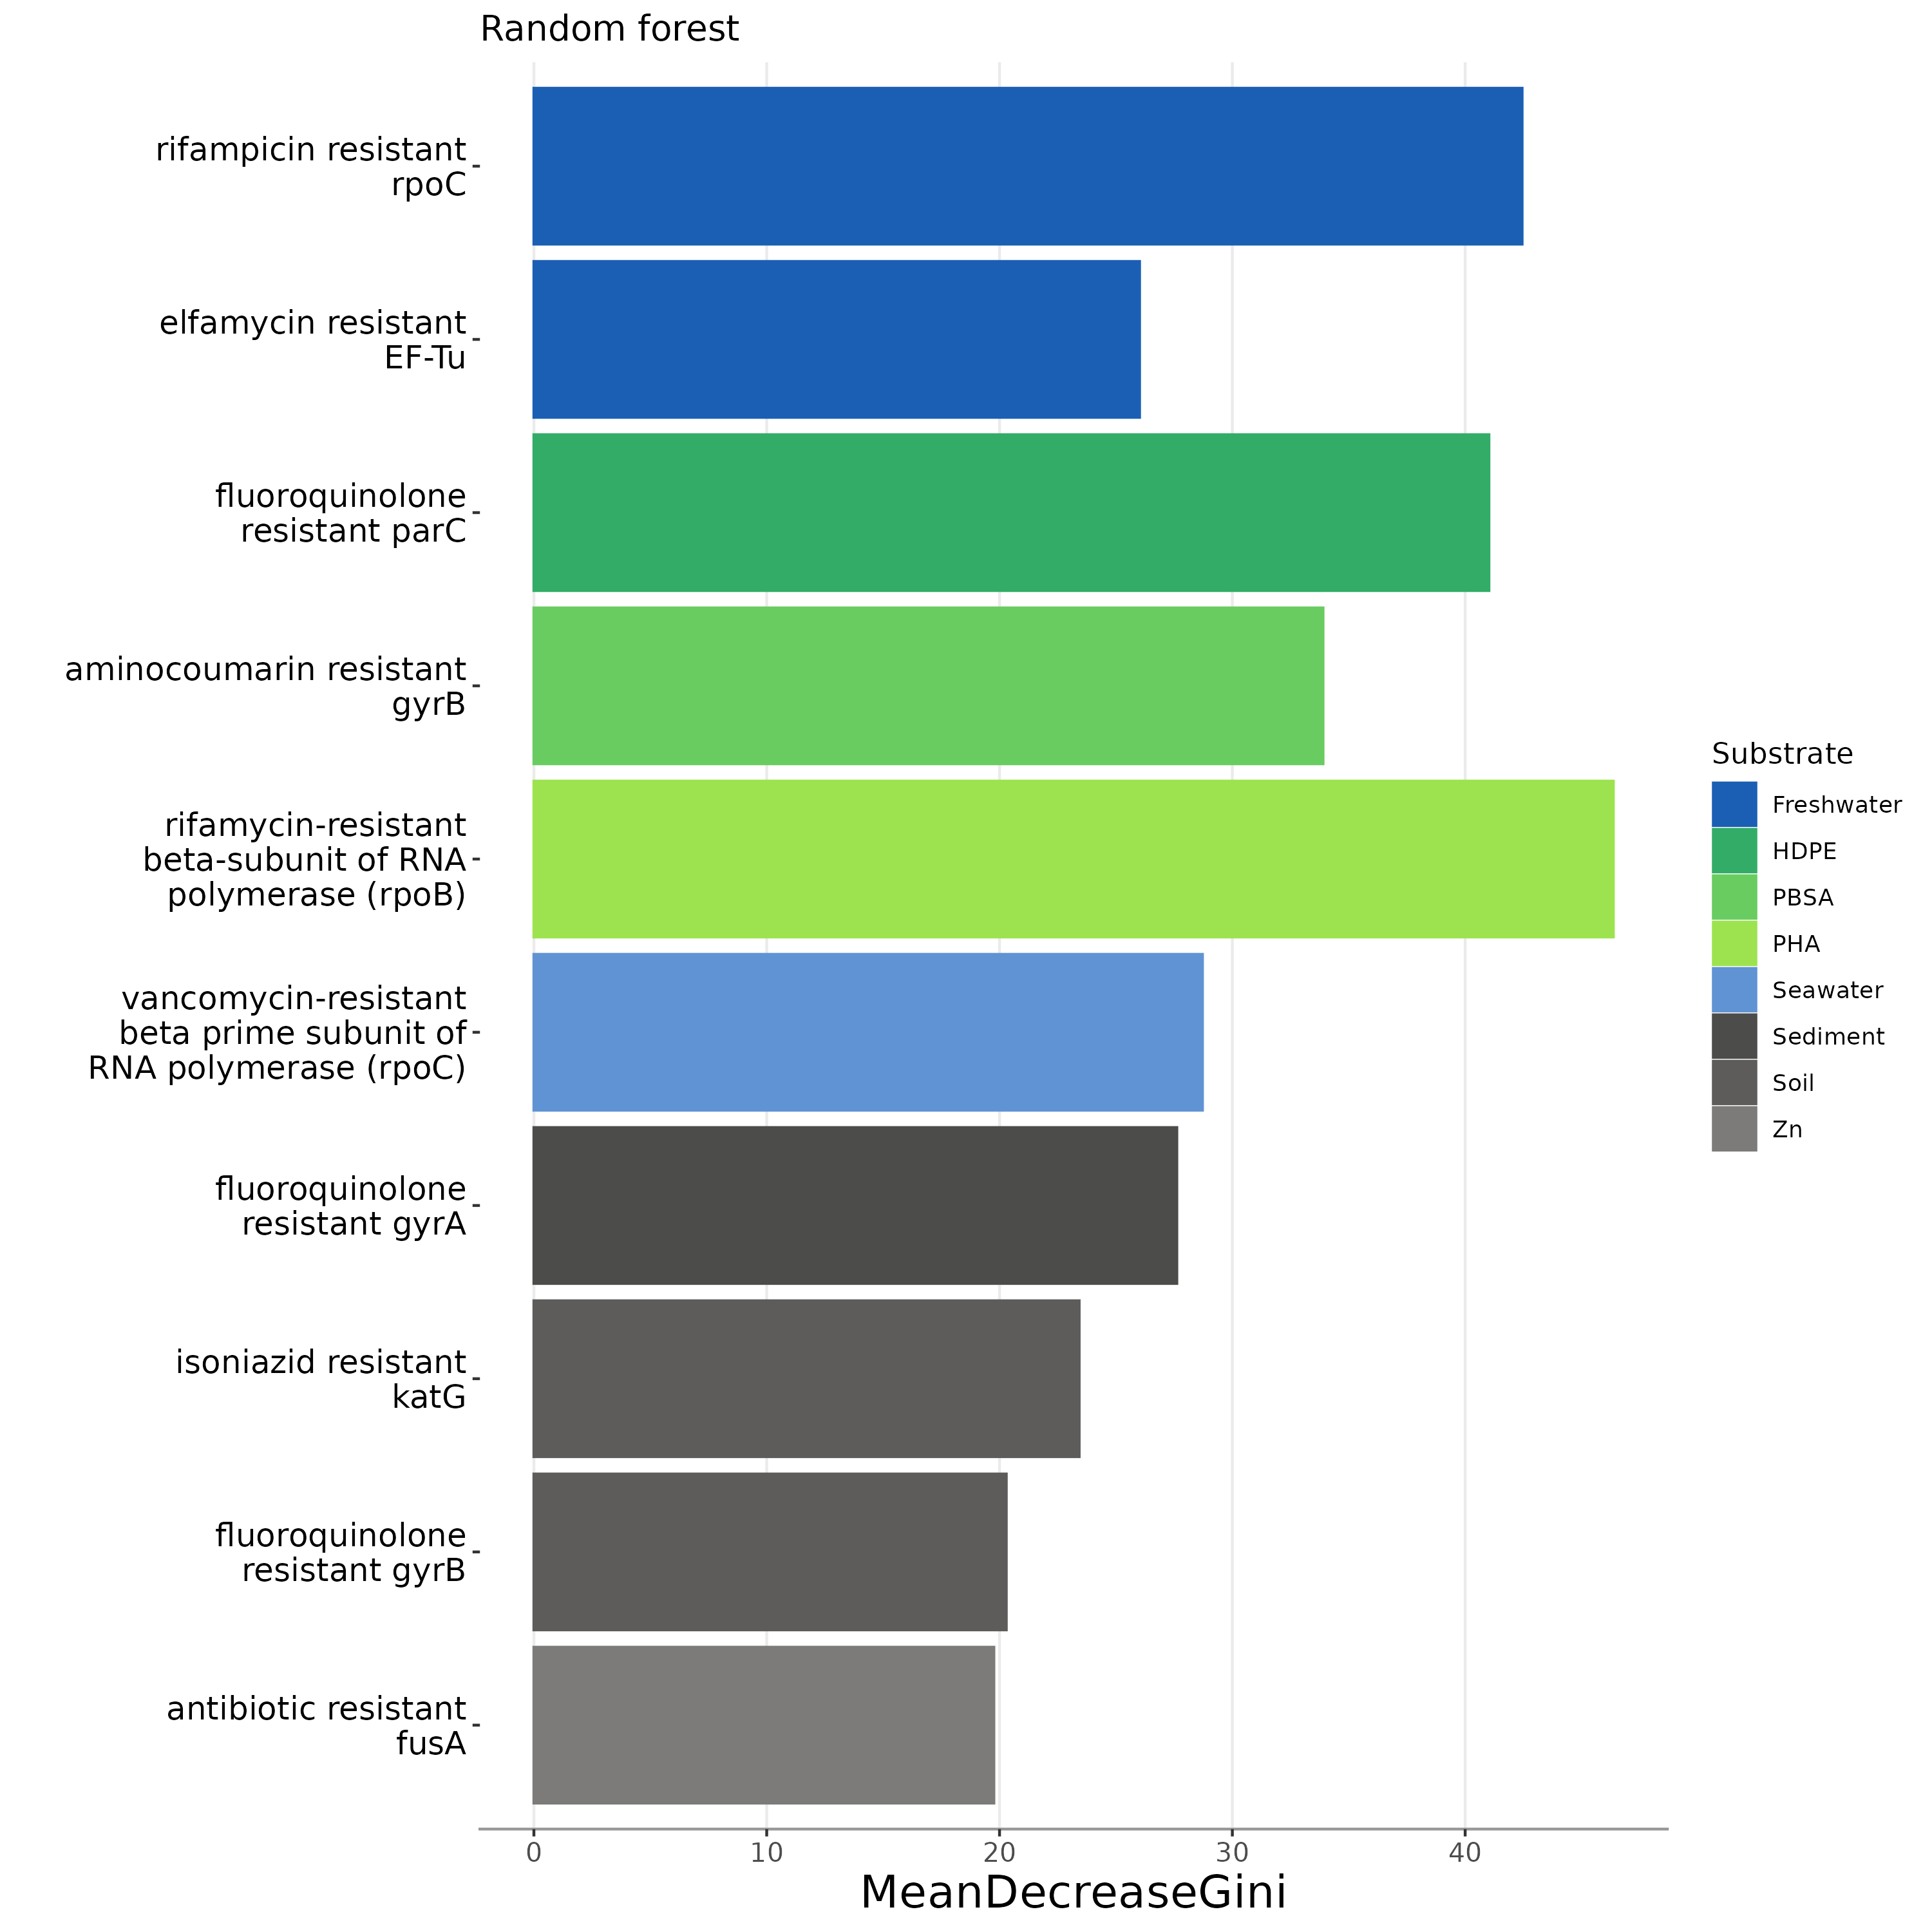
\includegraphics[width=0.5\textwidth]{figure/relative_forest_substrate_amr_bar.png}}
    \subfloat[Abundance plot, keep?.\label{amr_substrate_abund}]{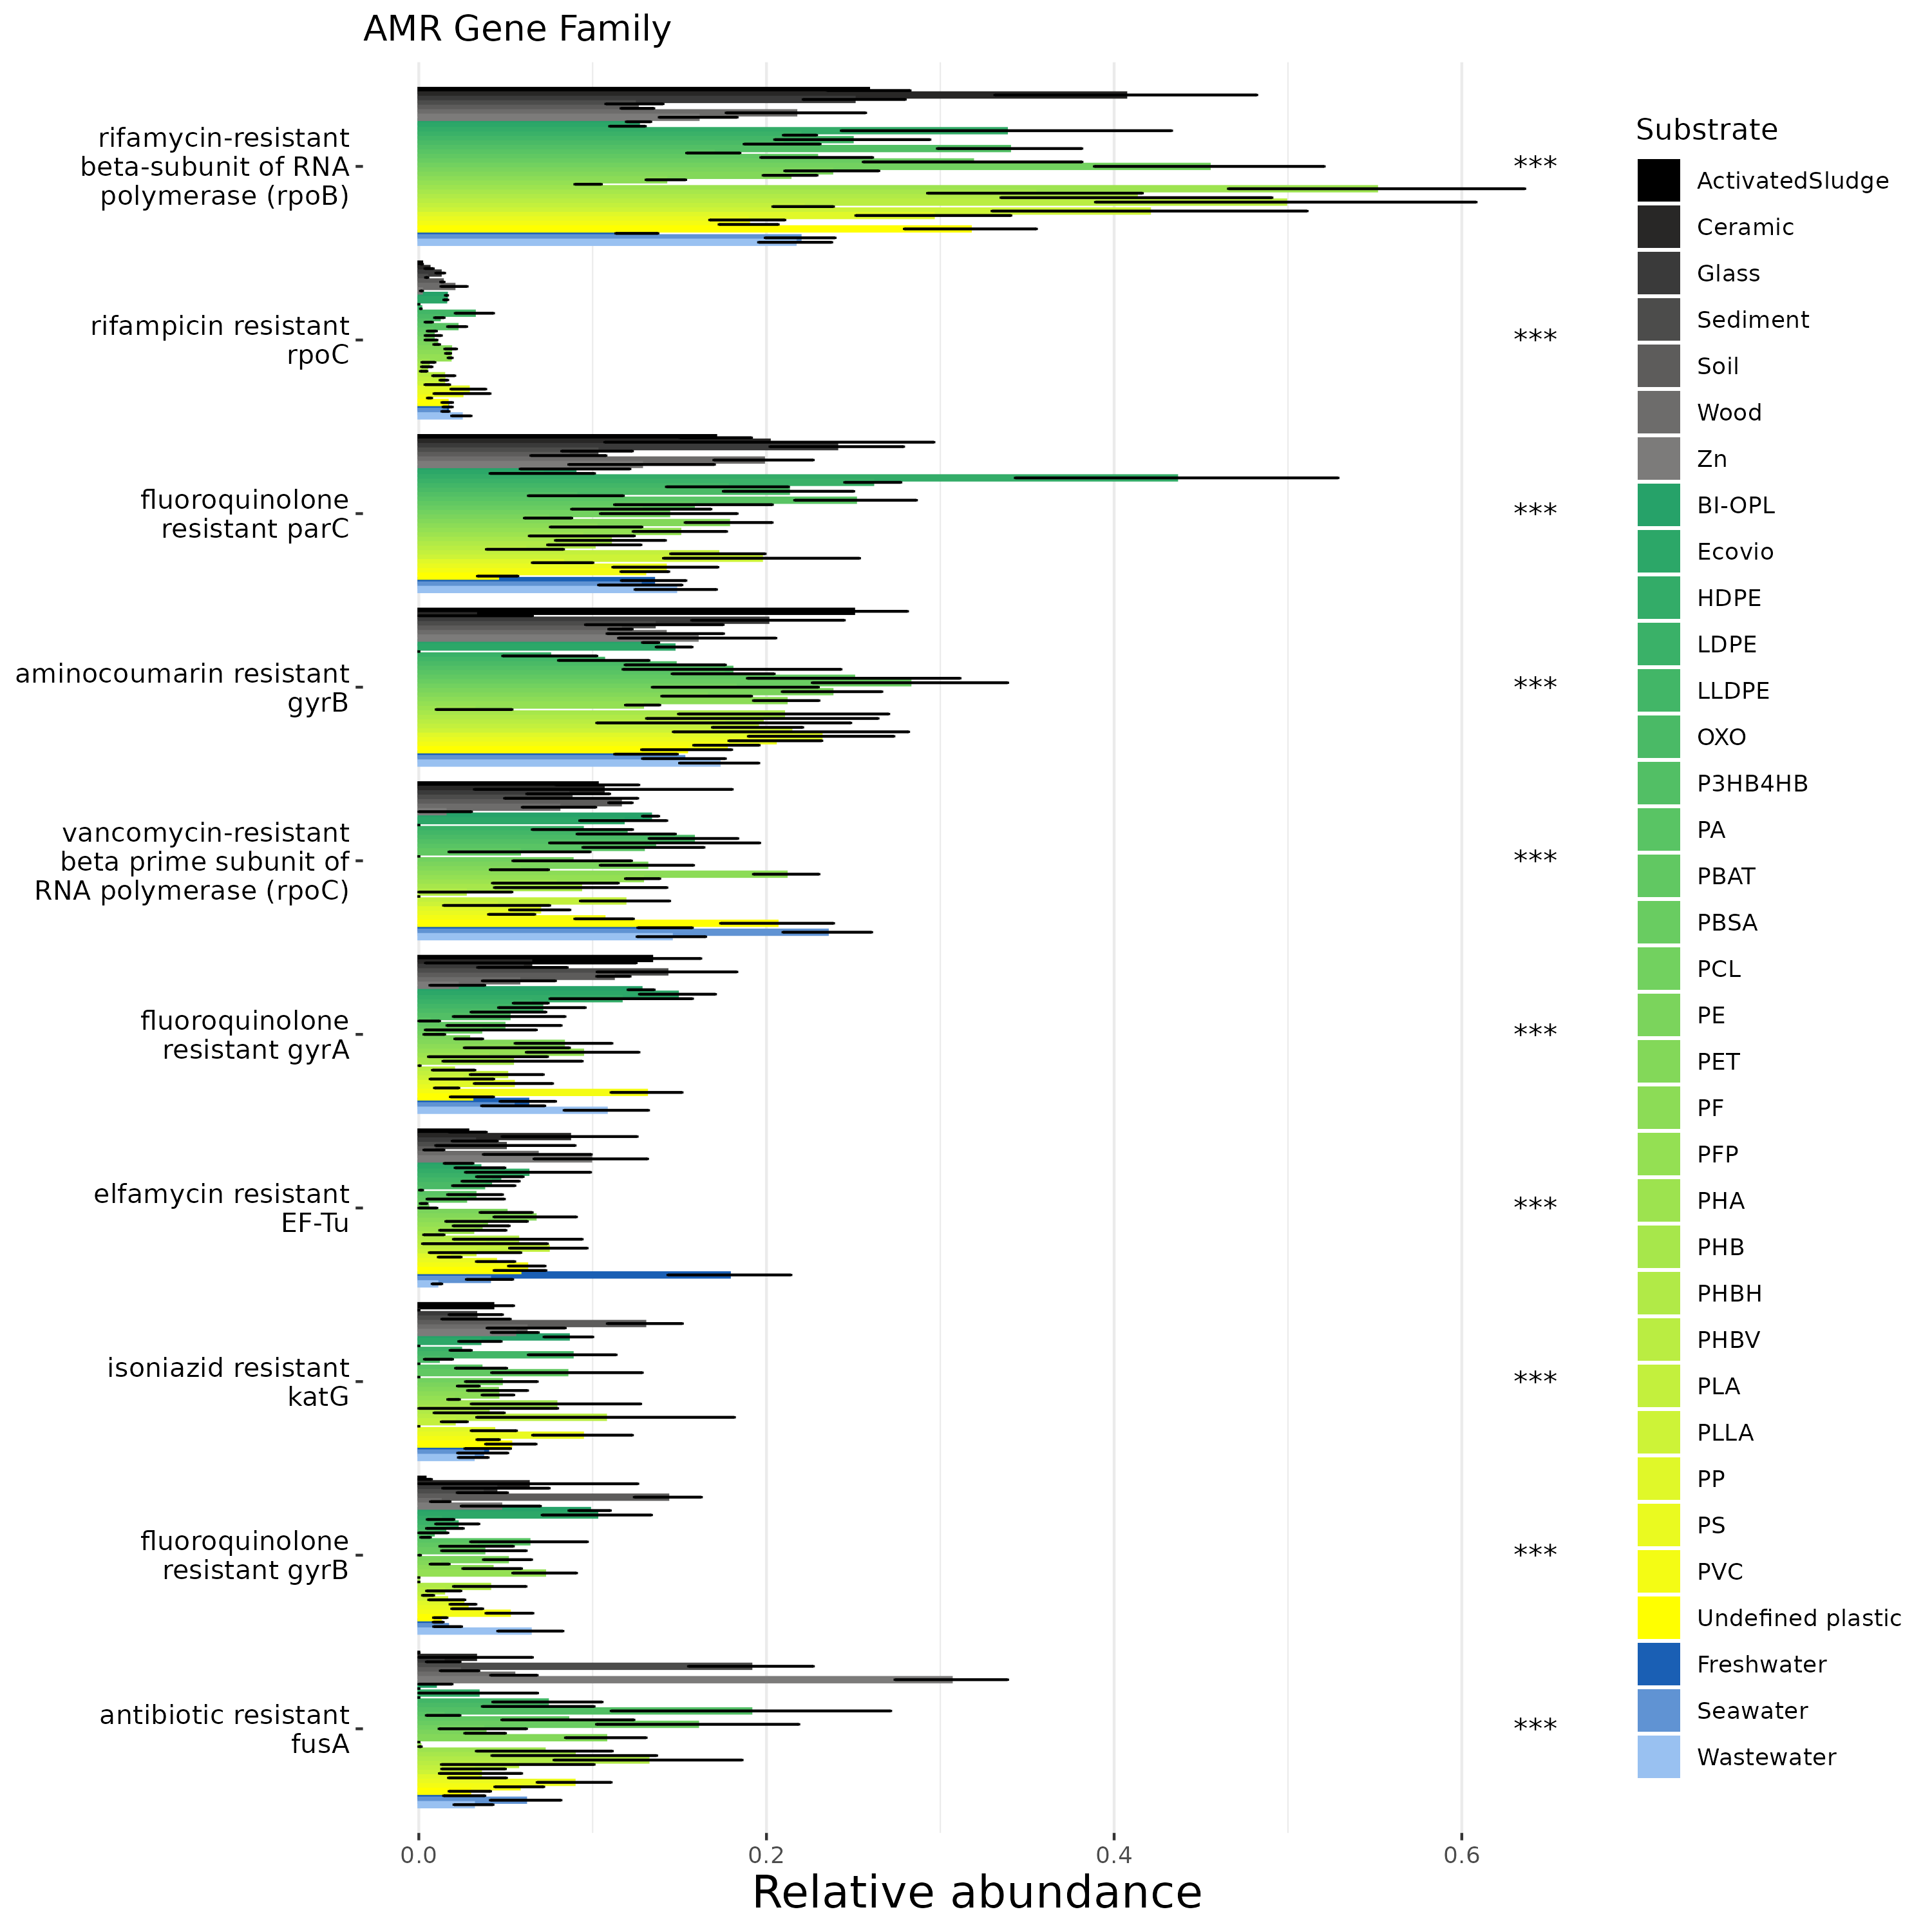
\includegraphics[width=0.5\textwidth]{figure/relative_forest_substrate_amr_abund.png}}
    \caption{AMR Substrate}
    \label{amr_substrate}
\end{figure}

\subsection{Mutations}
The following figures use the individual mutations, or combinations thereof, found in the samples as the grouping for which the random forest analysis was performed.
Figure \ref{snp_sampletype_bar} show the result of the analysis using the three different sampletypes as grouping, and as above only the non-plastic group and the water group are present. 
The significant mutations for the non-plastic group include several mutations in rpoB which confer resistance to rifampicin, as well as several in gyrA and parC which confer resistance to fluoroquinolones.
There is one combination of four mutations in rpoB which confer resistance to rifampicin. 
However, the abundance of these mutations is relatively low, as is shown in figure \ref{snp_sampletype_abund}.

\begin{figure}[h]
    \centering
    \subfloat[caption1.\label{snp_sampletype_bar}]{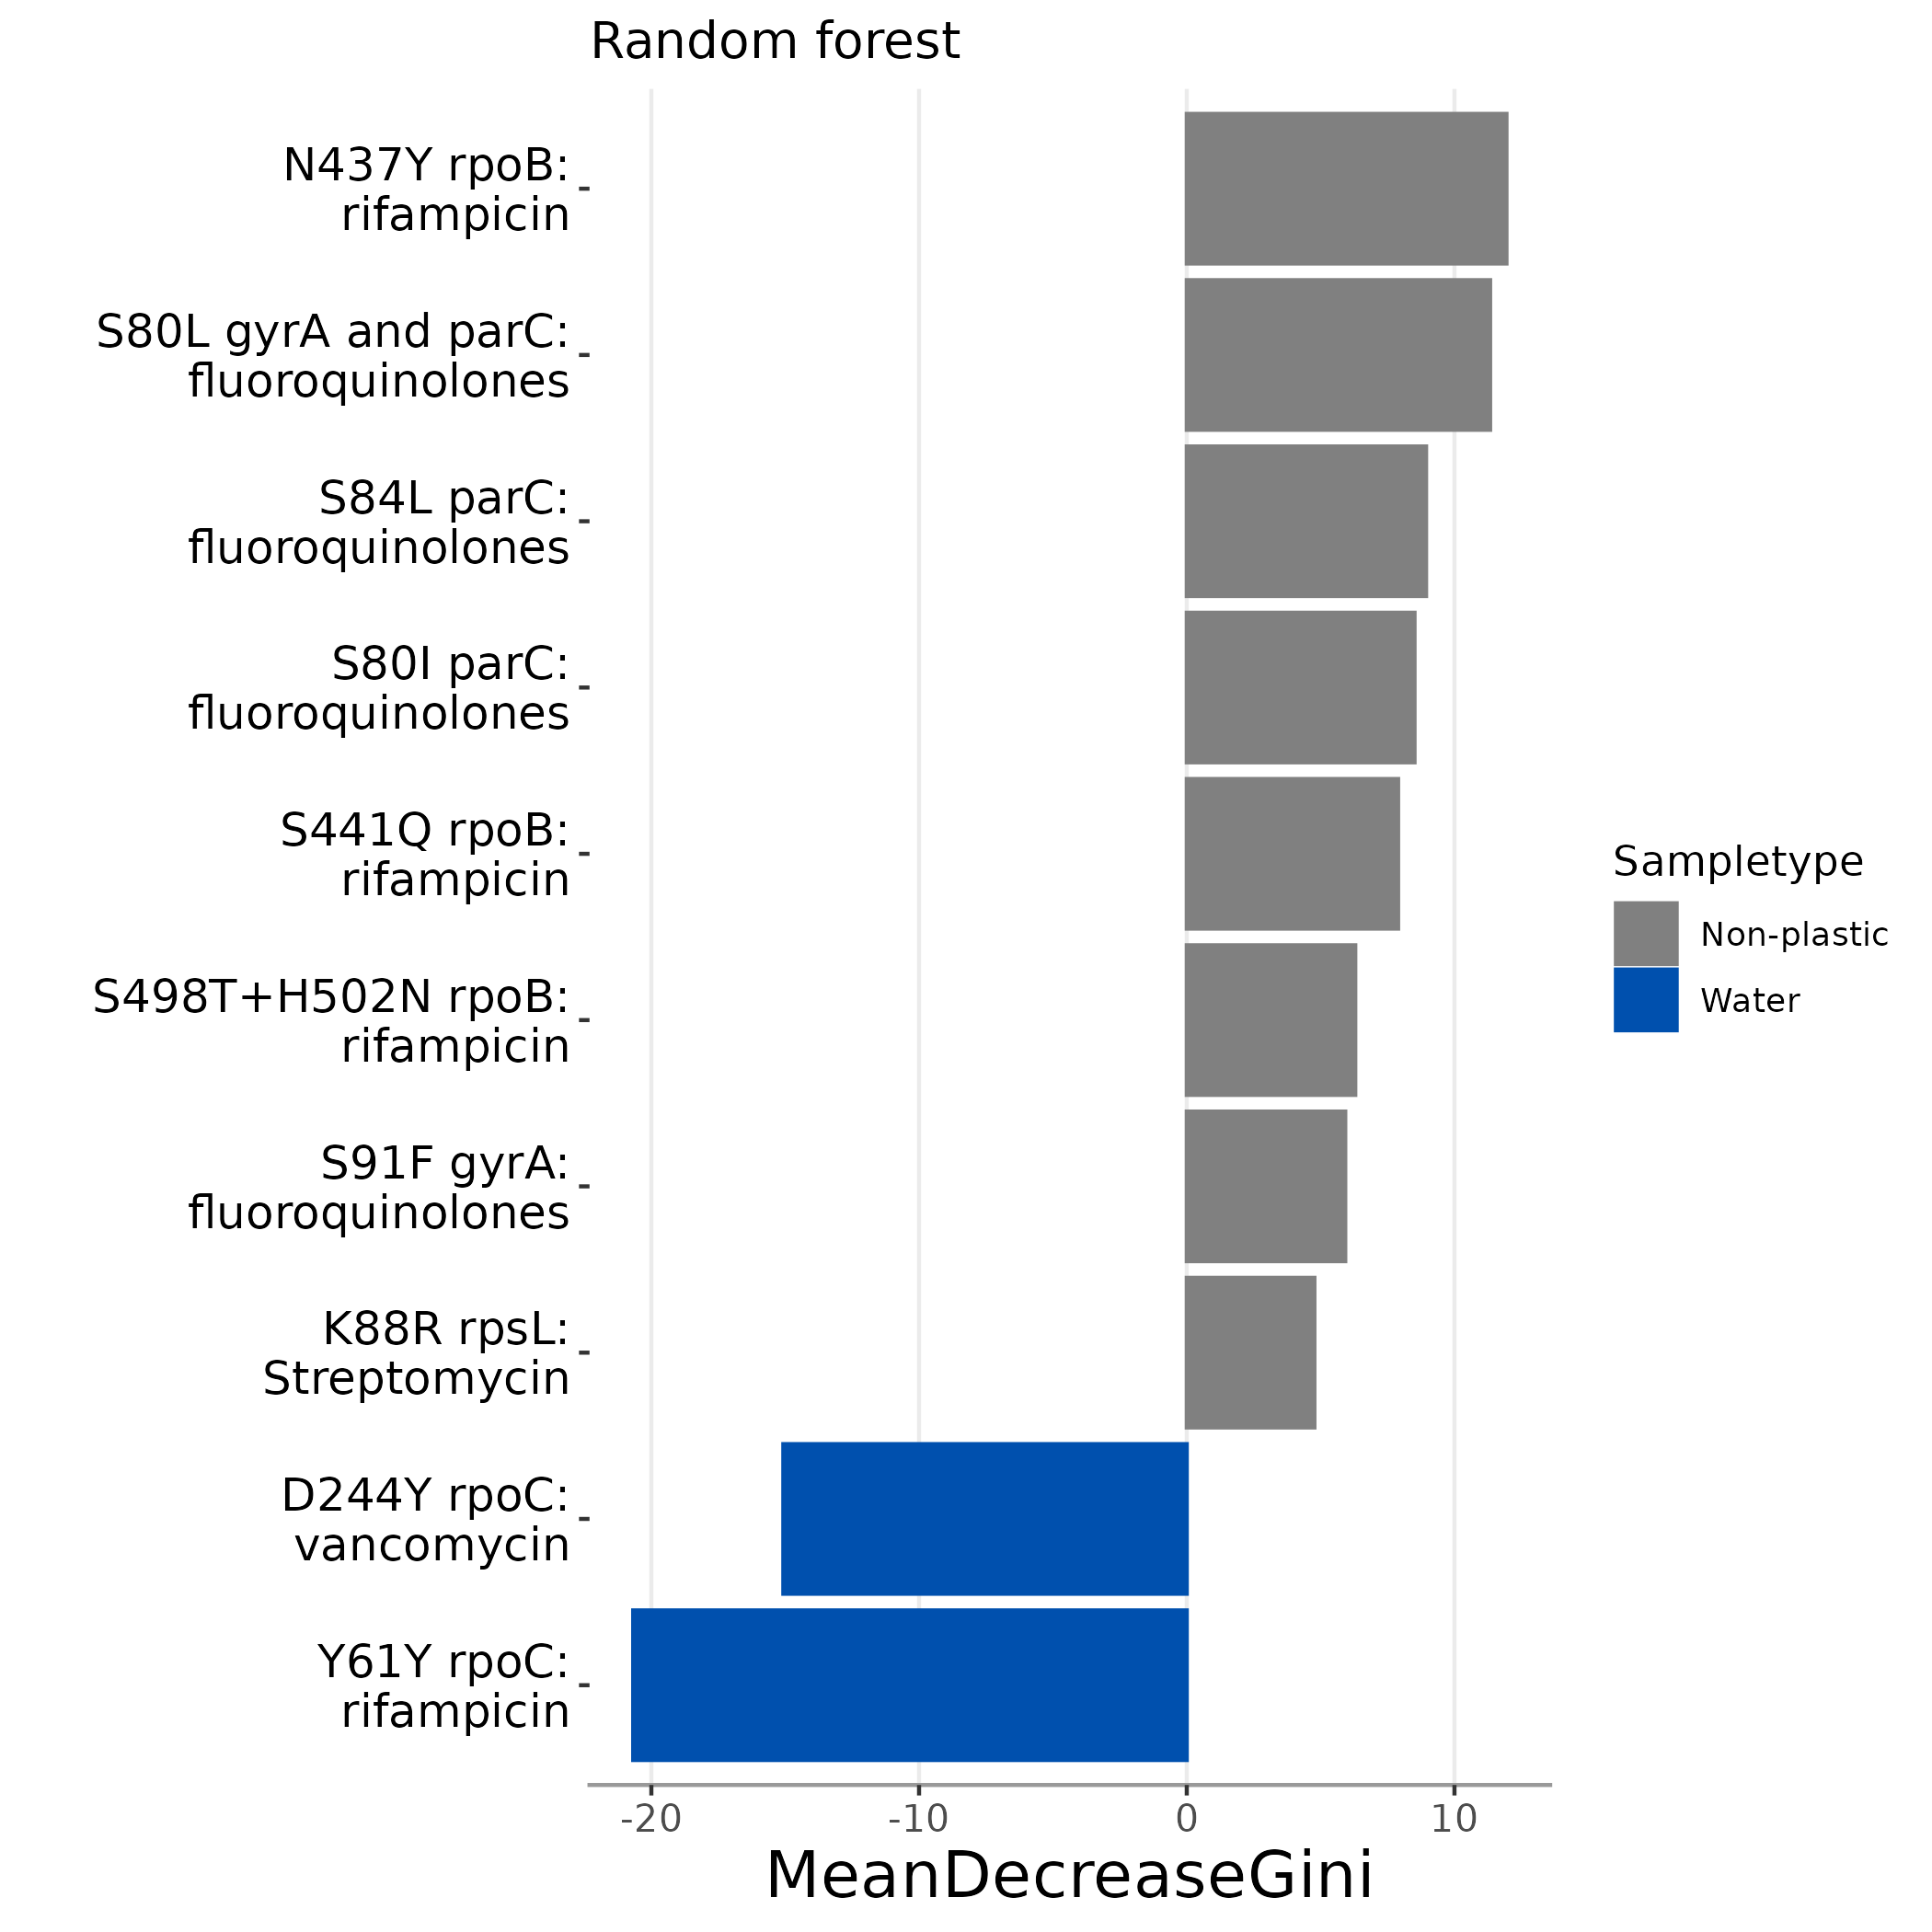
\includegraphics[width=0.5\textwidth]{figure/relative_forest_sampletype_snps_bar.png}}
    \subfloat[TODO: Remove?.\label{snp_sampletype_abund}]{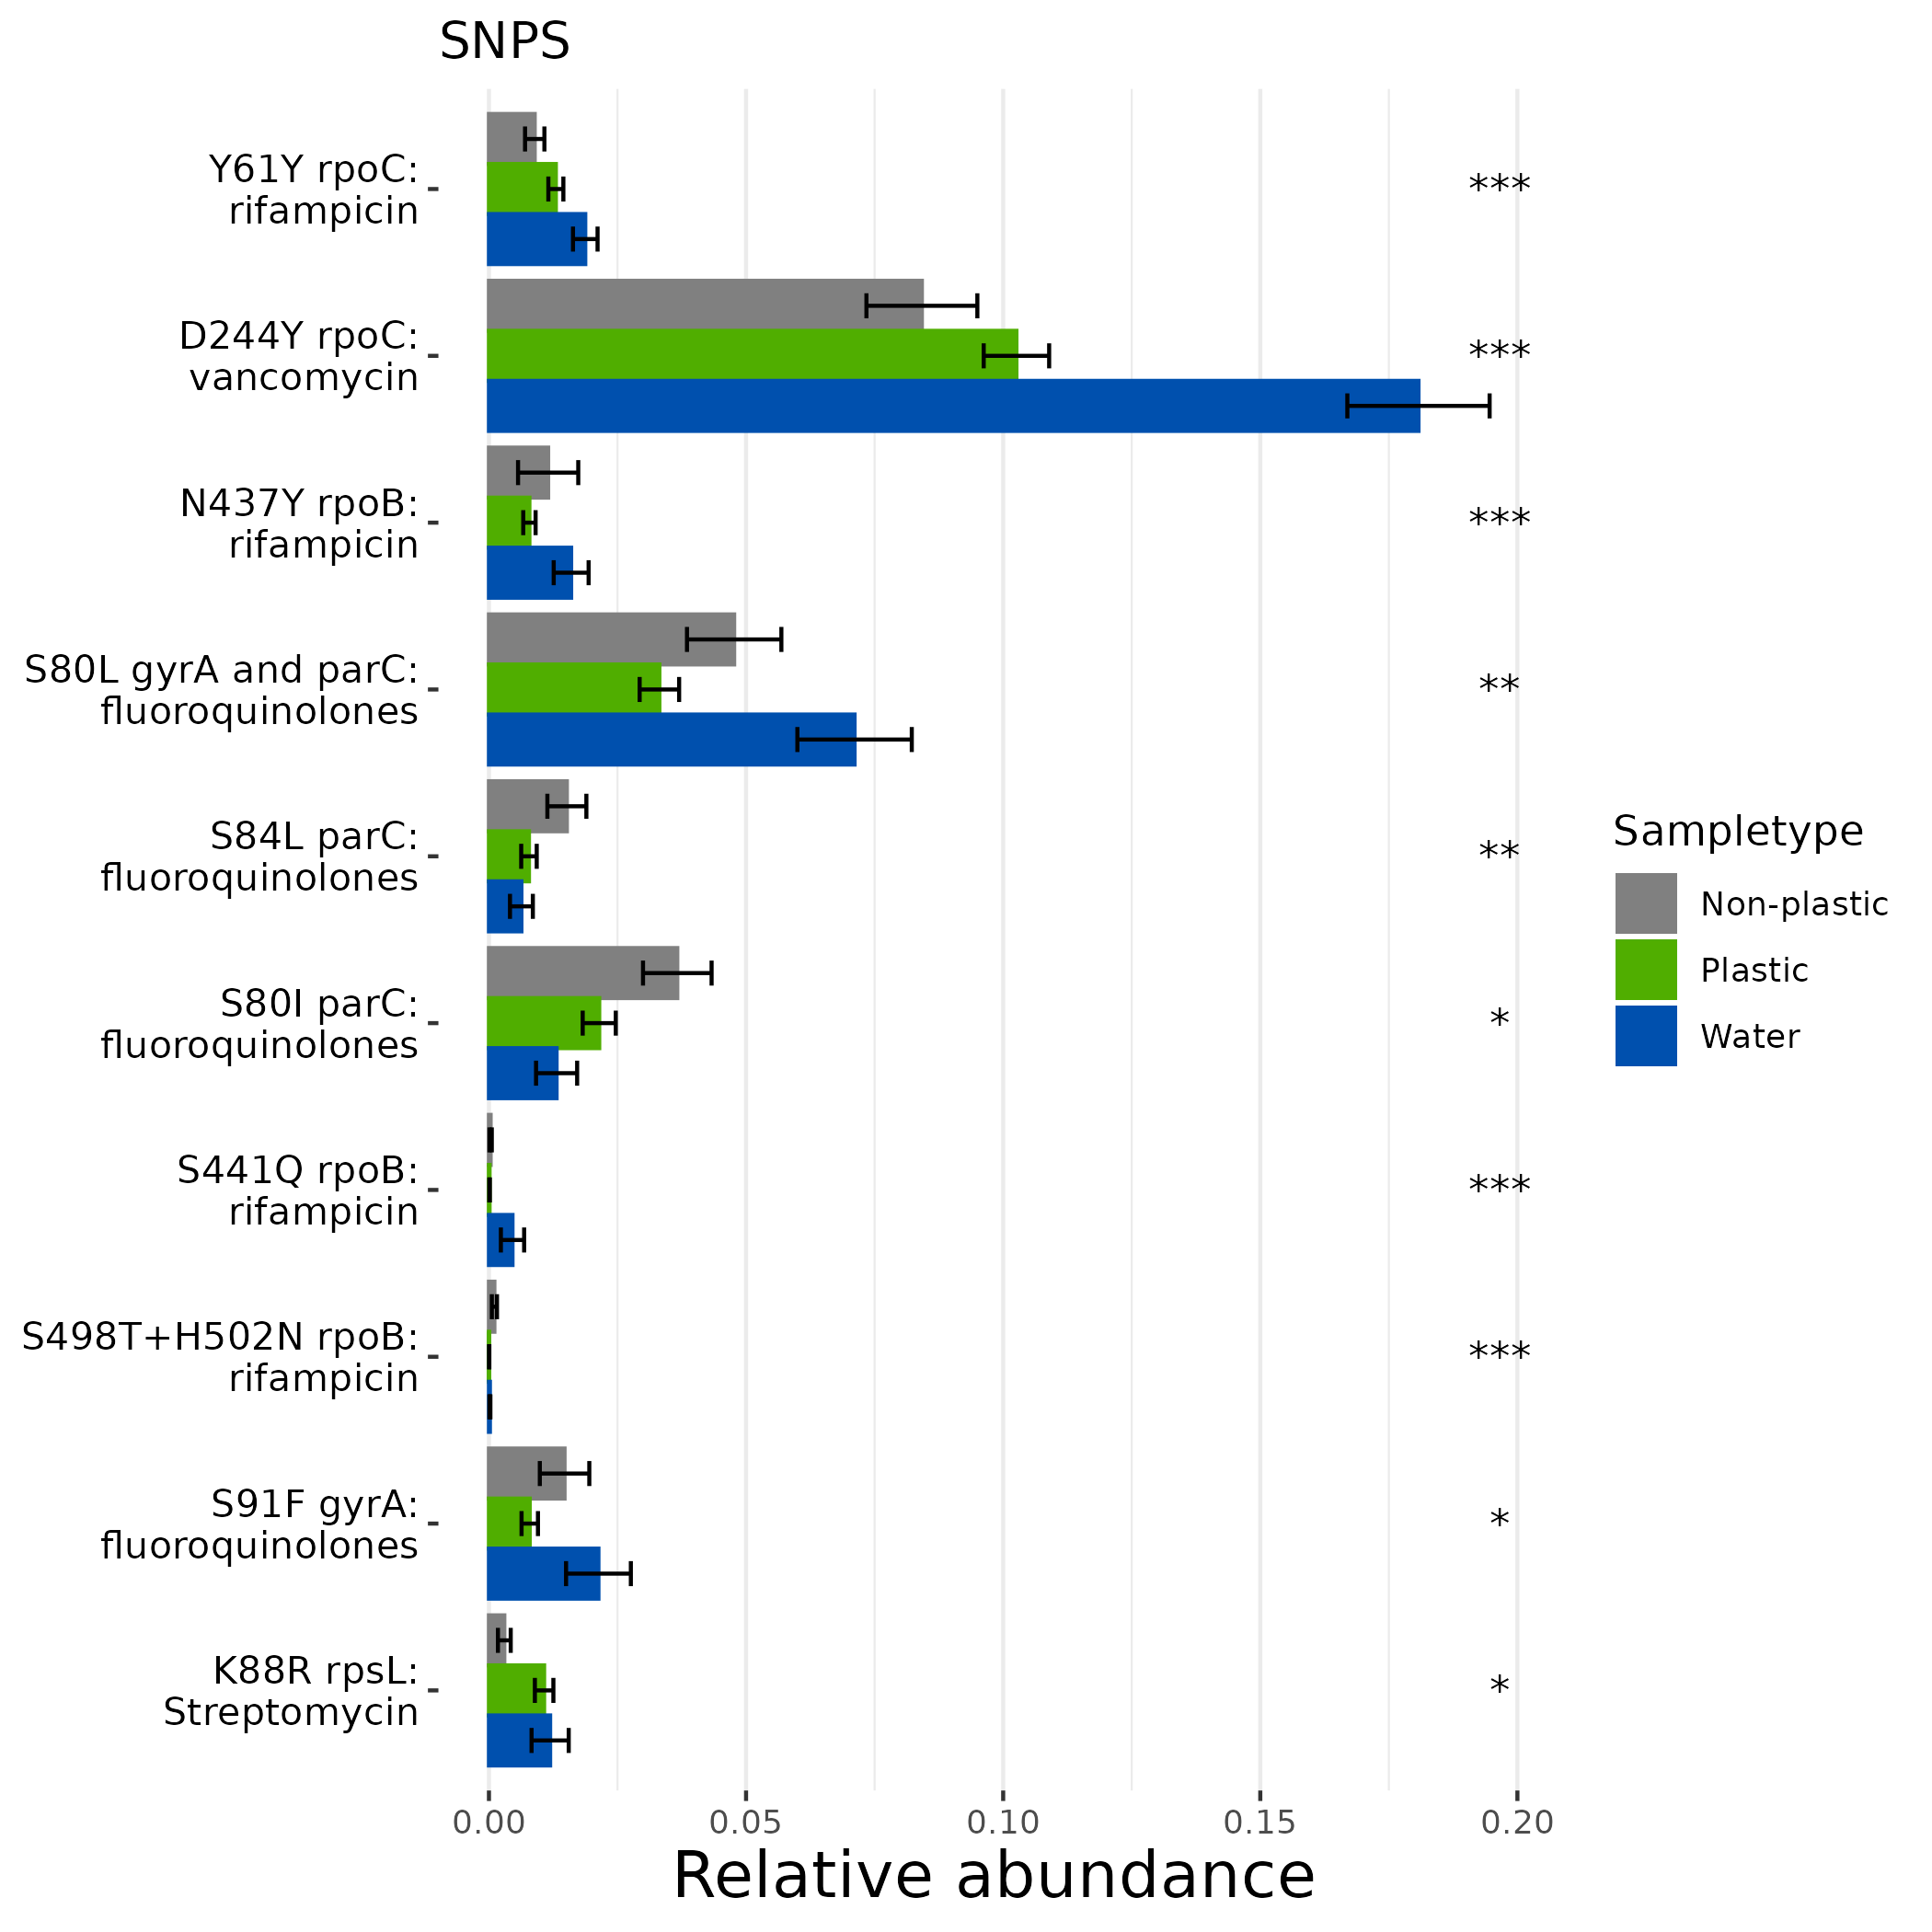
\includegraphics[width=0.5\textwidth]{figure/relative_forest_sampletype_snps_abund.png}}
    \caption{SNPS Sampletype}
    \label{snps_sampletype}
\end{figure}

When instead the different substrates is used as the grouping variable in the random forest analysis, the mutations with the highest mean decrease gini importance are not the same, however many of the genes and the resistances they confer are the same. These include parC (fluoroquinolones), rpoB (rifampicin), rpoC (rifampicin or vancomycin), gyrB (aminocoumarin), and are shown in figure \ref{snp_substrate_bar}. The mutations in EF-Tu, which confer resistance to pulvomycin, are not present in the previous plot, and may be used to identify ceramic as a substrate.\todo{note however that there are only 3 ceramic samples used in this study, which may skew the results.}

\begin{figure}[h]
    \centering
    \subfloat[caption1.\label{snp_substrate_bar}]{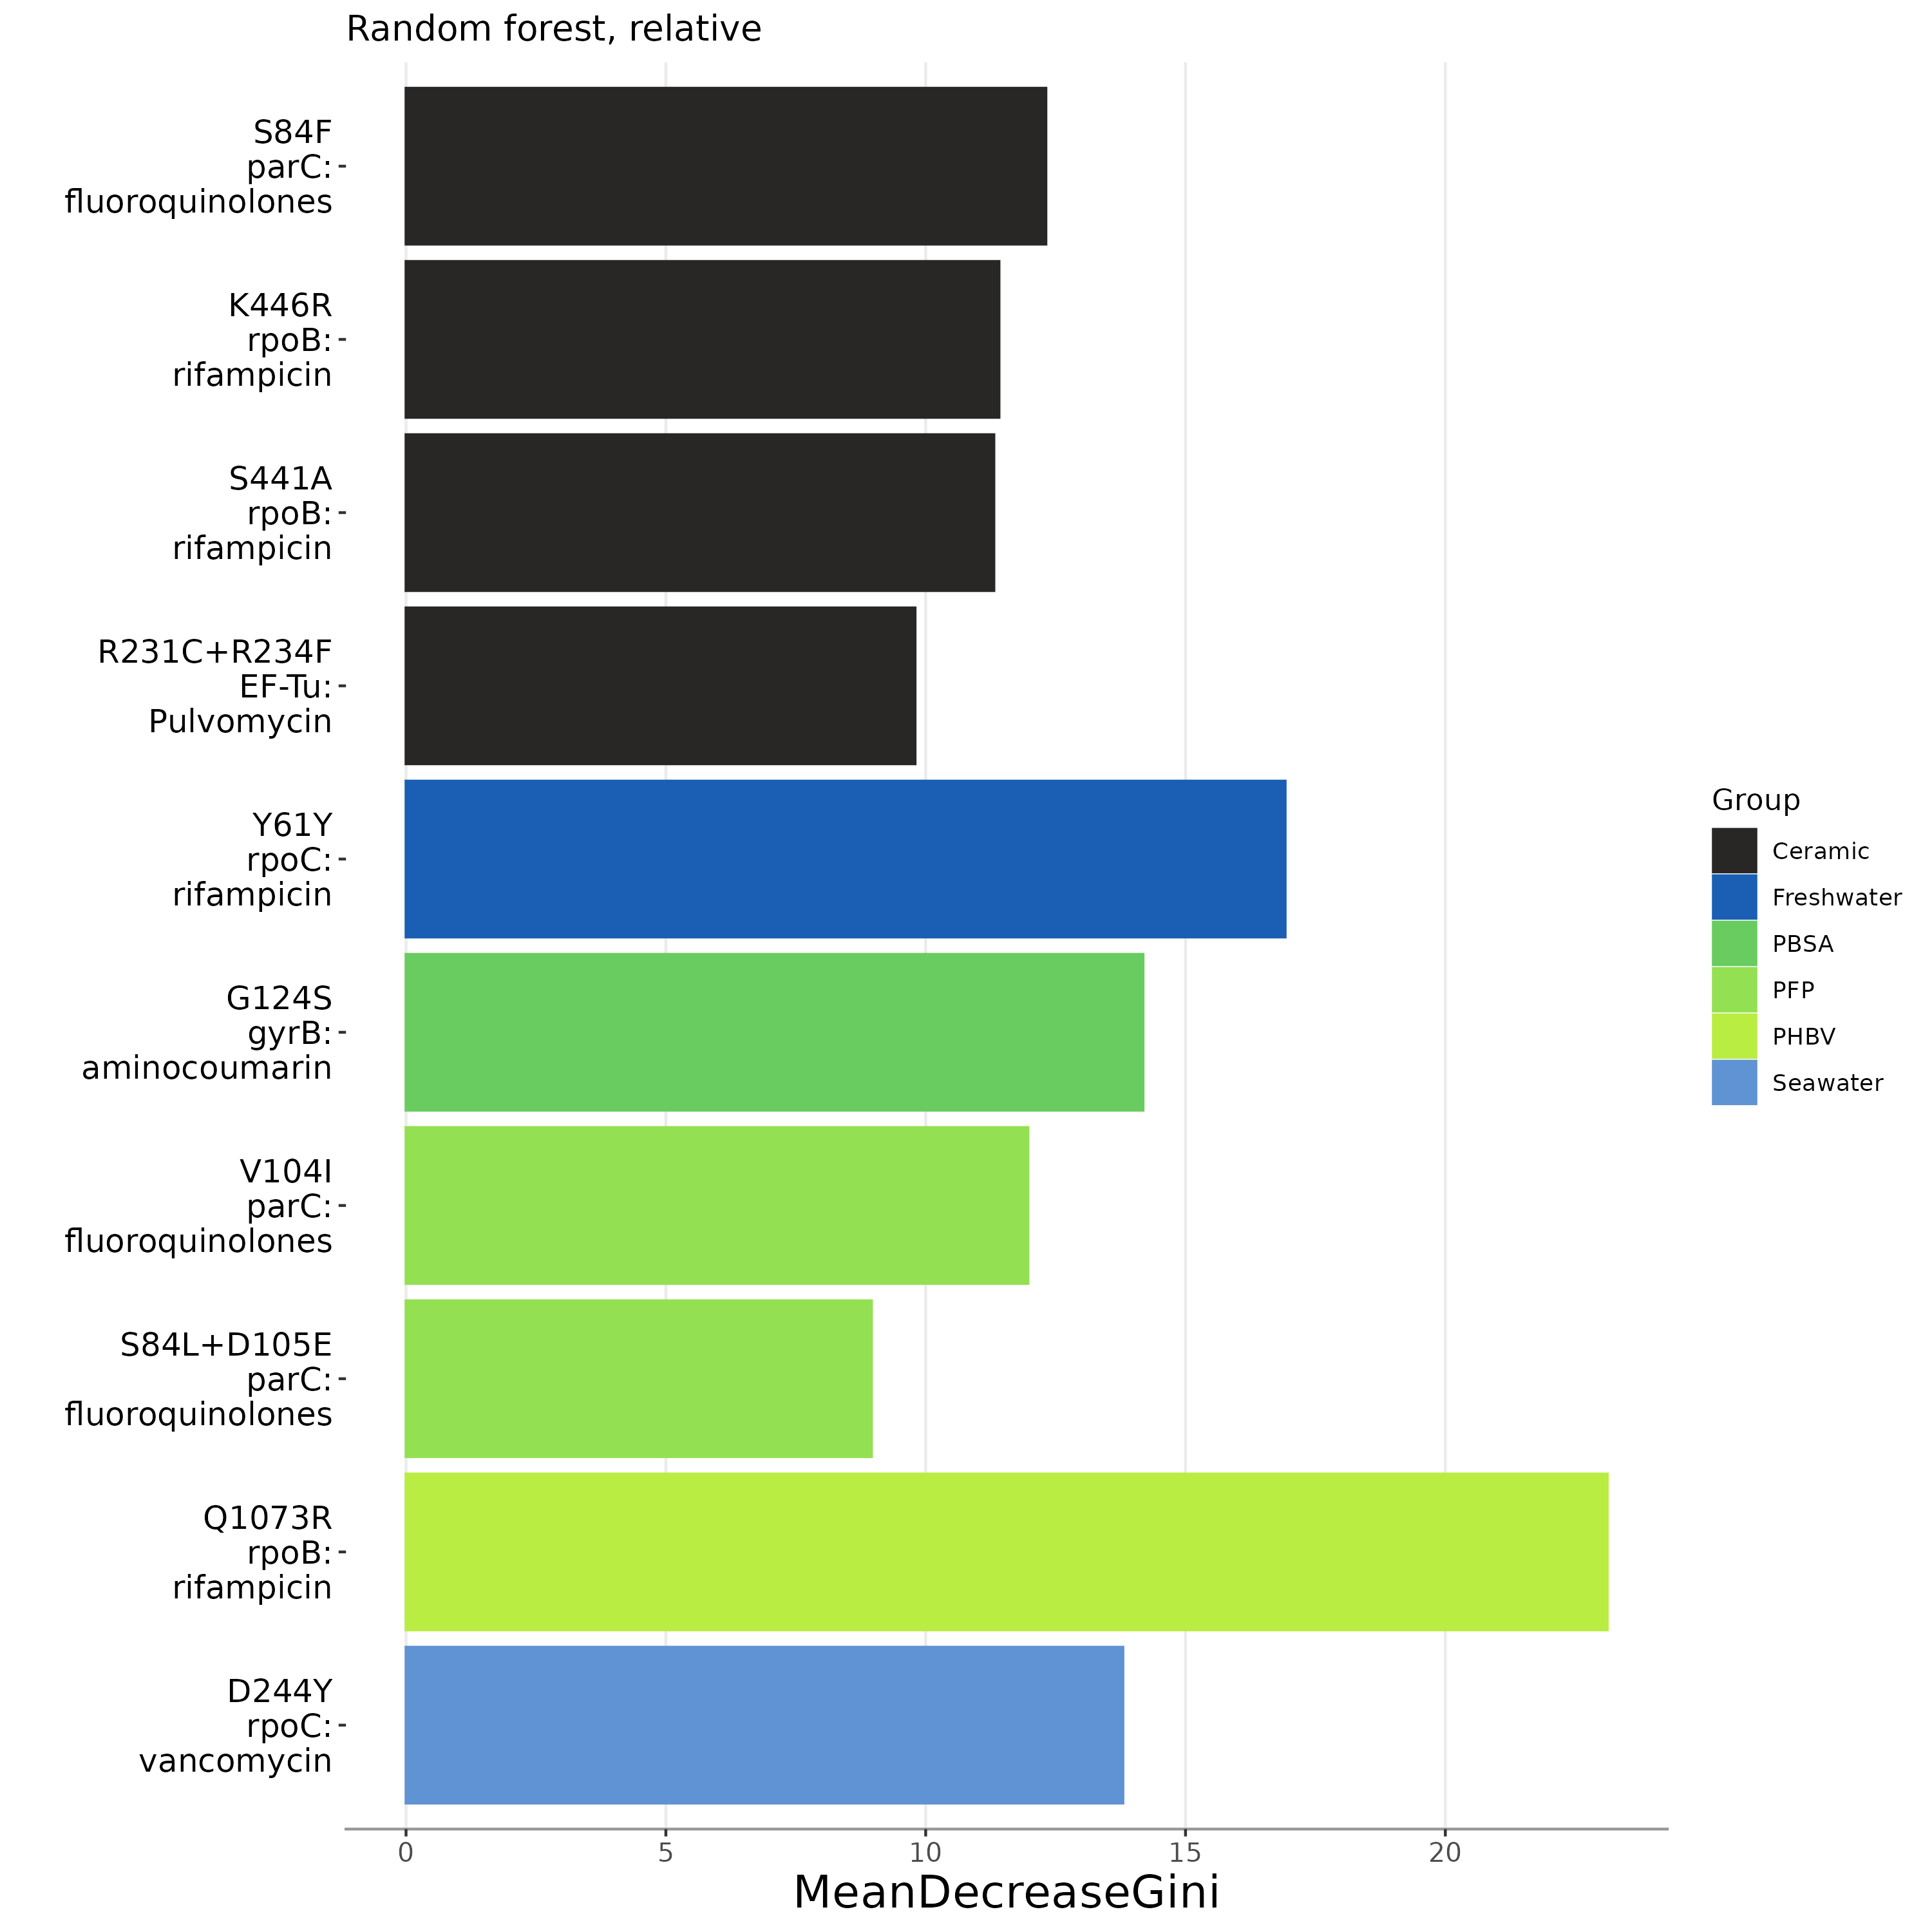
\includegraphics[width=0.5\textwidth]{figure/relative_forest_substrate_snps_bar.png}}
    \subfloat[caption2.\label{snp_substrate_abund}]{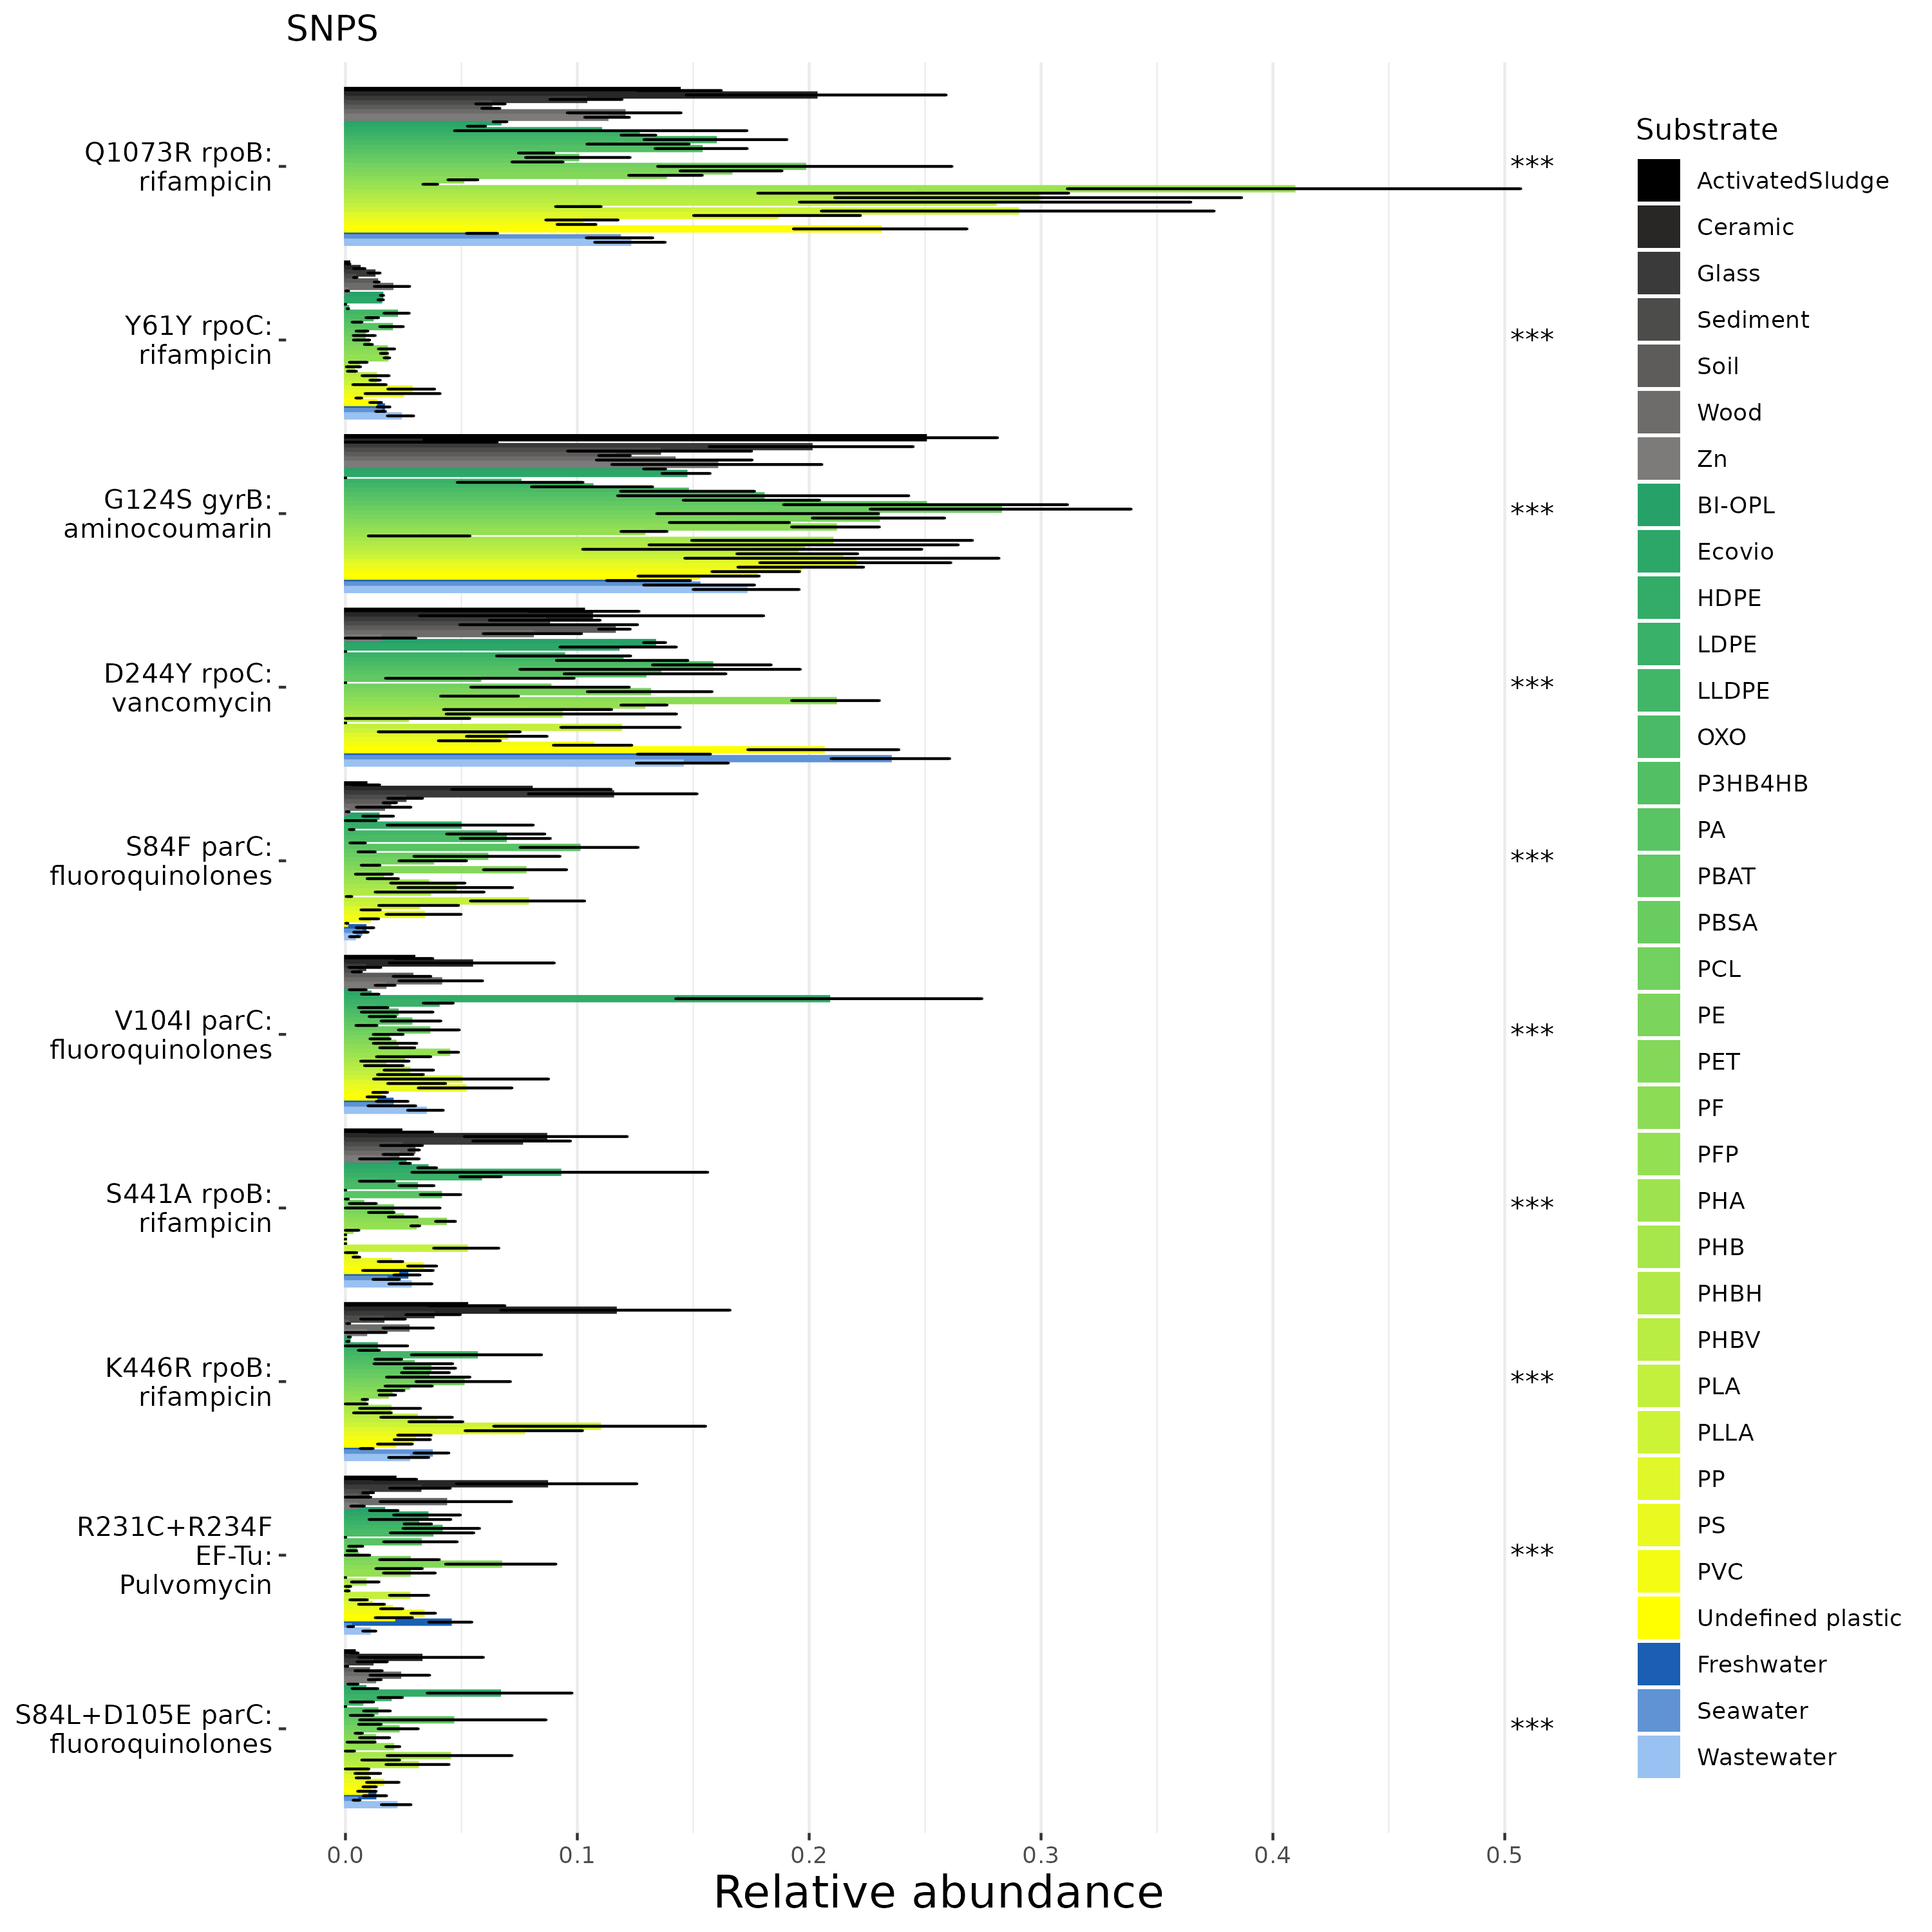
\includegraphics[width=0.5\textwidth]{figure/relative_forest_substrate_snps_abund.png}}
    \caption{SNPS Substrate}
    \label{snps_substrate}
\end{figure}

\section{Taxonomic Abundance}
The taxonomic abundance of all samples is shown in figure \ref{tax_plot}. The plot show the taxnomic abundance at the phylum level, and is divided by ecosystem type and sampletype. 
The ecosystem type is the environment in which the sample was taken, regardless of the sampletype. For example, some of the samples were taken in the Pacific Ocean, and there both plastic substrates and seawater substrates were analysed.
The figure shows that the largest difference is between the different ecosystems, but that sampletype also matters.\todo{Very unsure of how to analuze these plots, since we lack statistics for them.}
The most abundant phyla in all ecosystems are proteobacteria, except in the wastewater samples where SAR is most abundant in most of the samples.

%there are differences between the different ecosystems, but that there is relatively small differences between the different sampletypes and substrates. 

Figure \ref{tax_plot_substrate} show the same plot, but this time also divided by substrate.\todo{Which of these should be present? Could turn the whole plot 90° on the page to be easier to read? see fig \ref{tax_plot_substrate_flip}}

\begin{figure}[h]
    \centering
    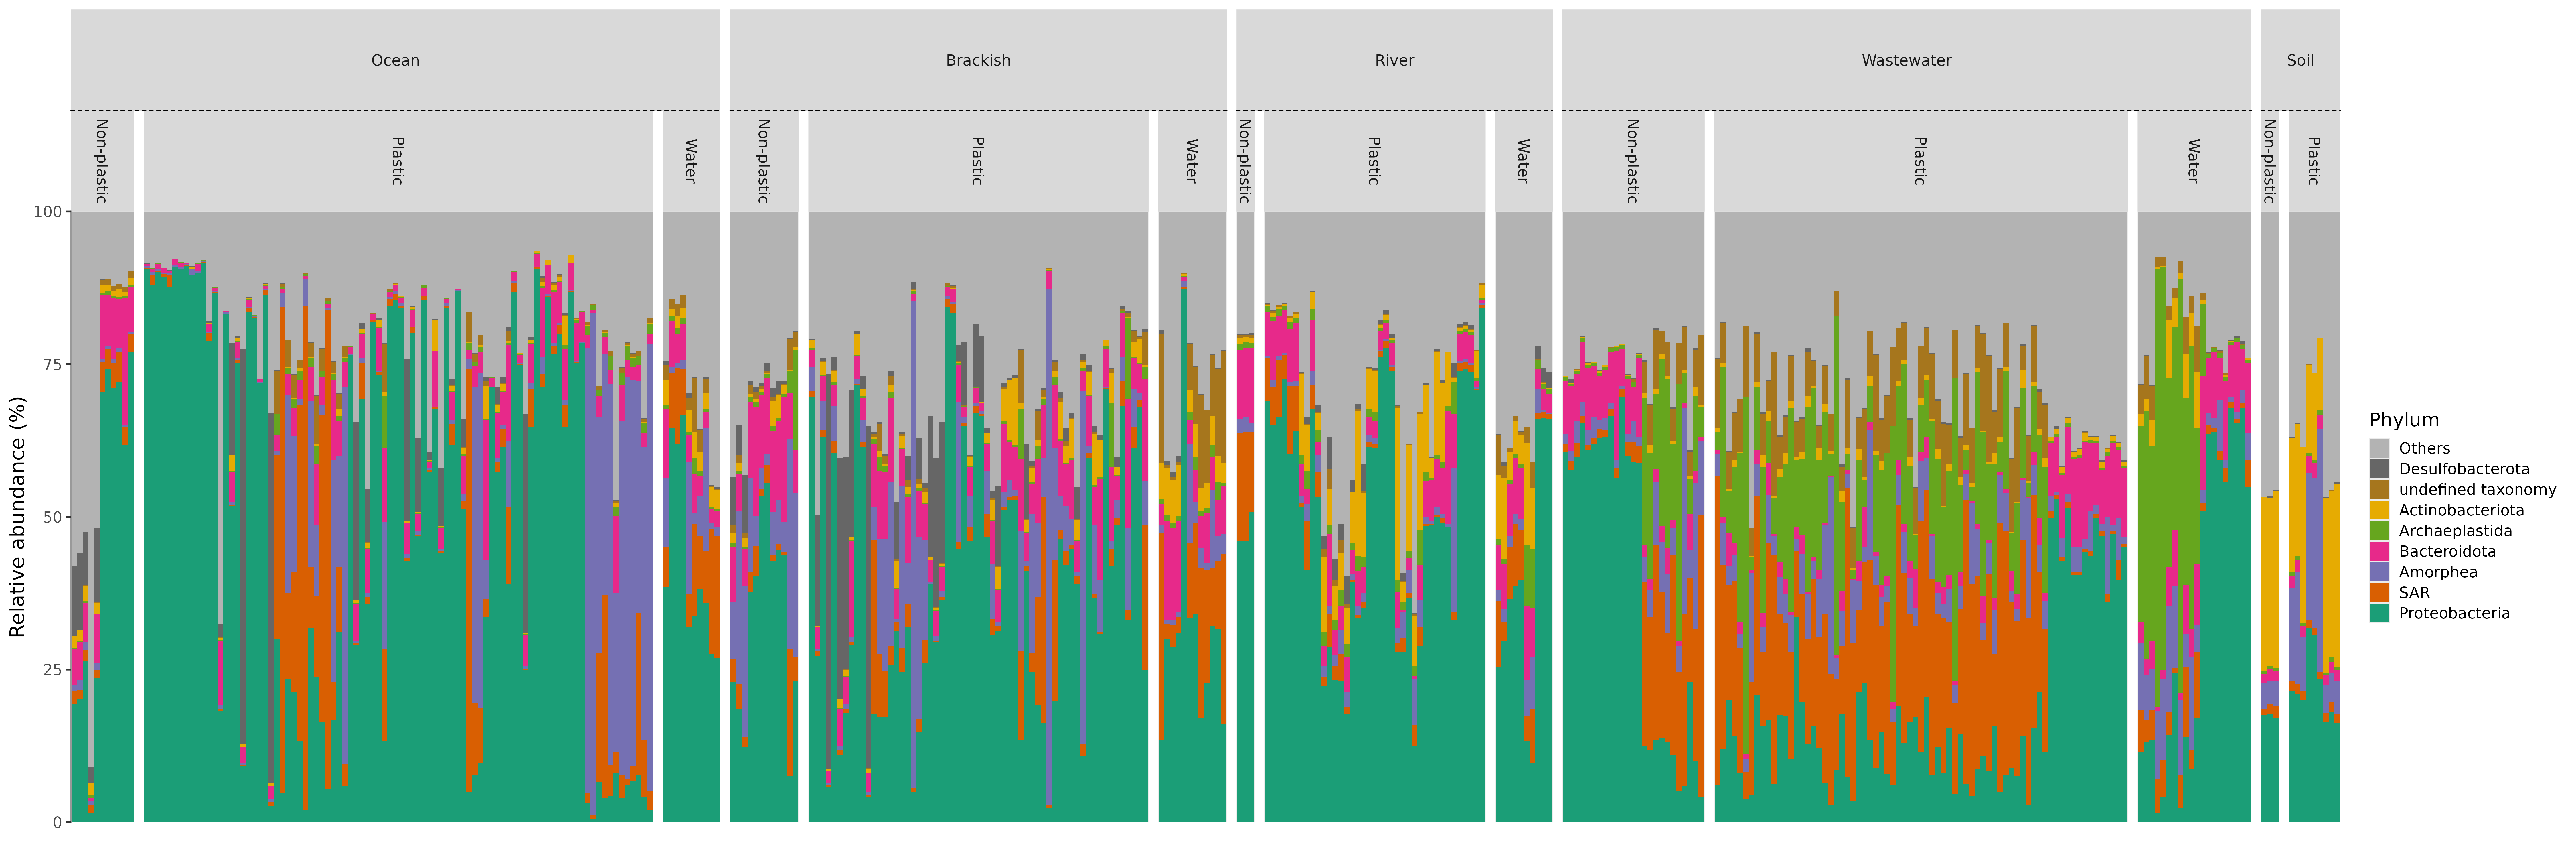
\includegraphics[width = \textwidth]{figure/tax_phylum_ecosystem_sampletype.png}
    \caption{Taxonomic abundance for all samples at the Phylum level, divided by ecosystem type and sampletype}
    \label{tax_plot}
\end{figure}

\begin{figure}[h]
    \centering
    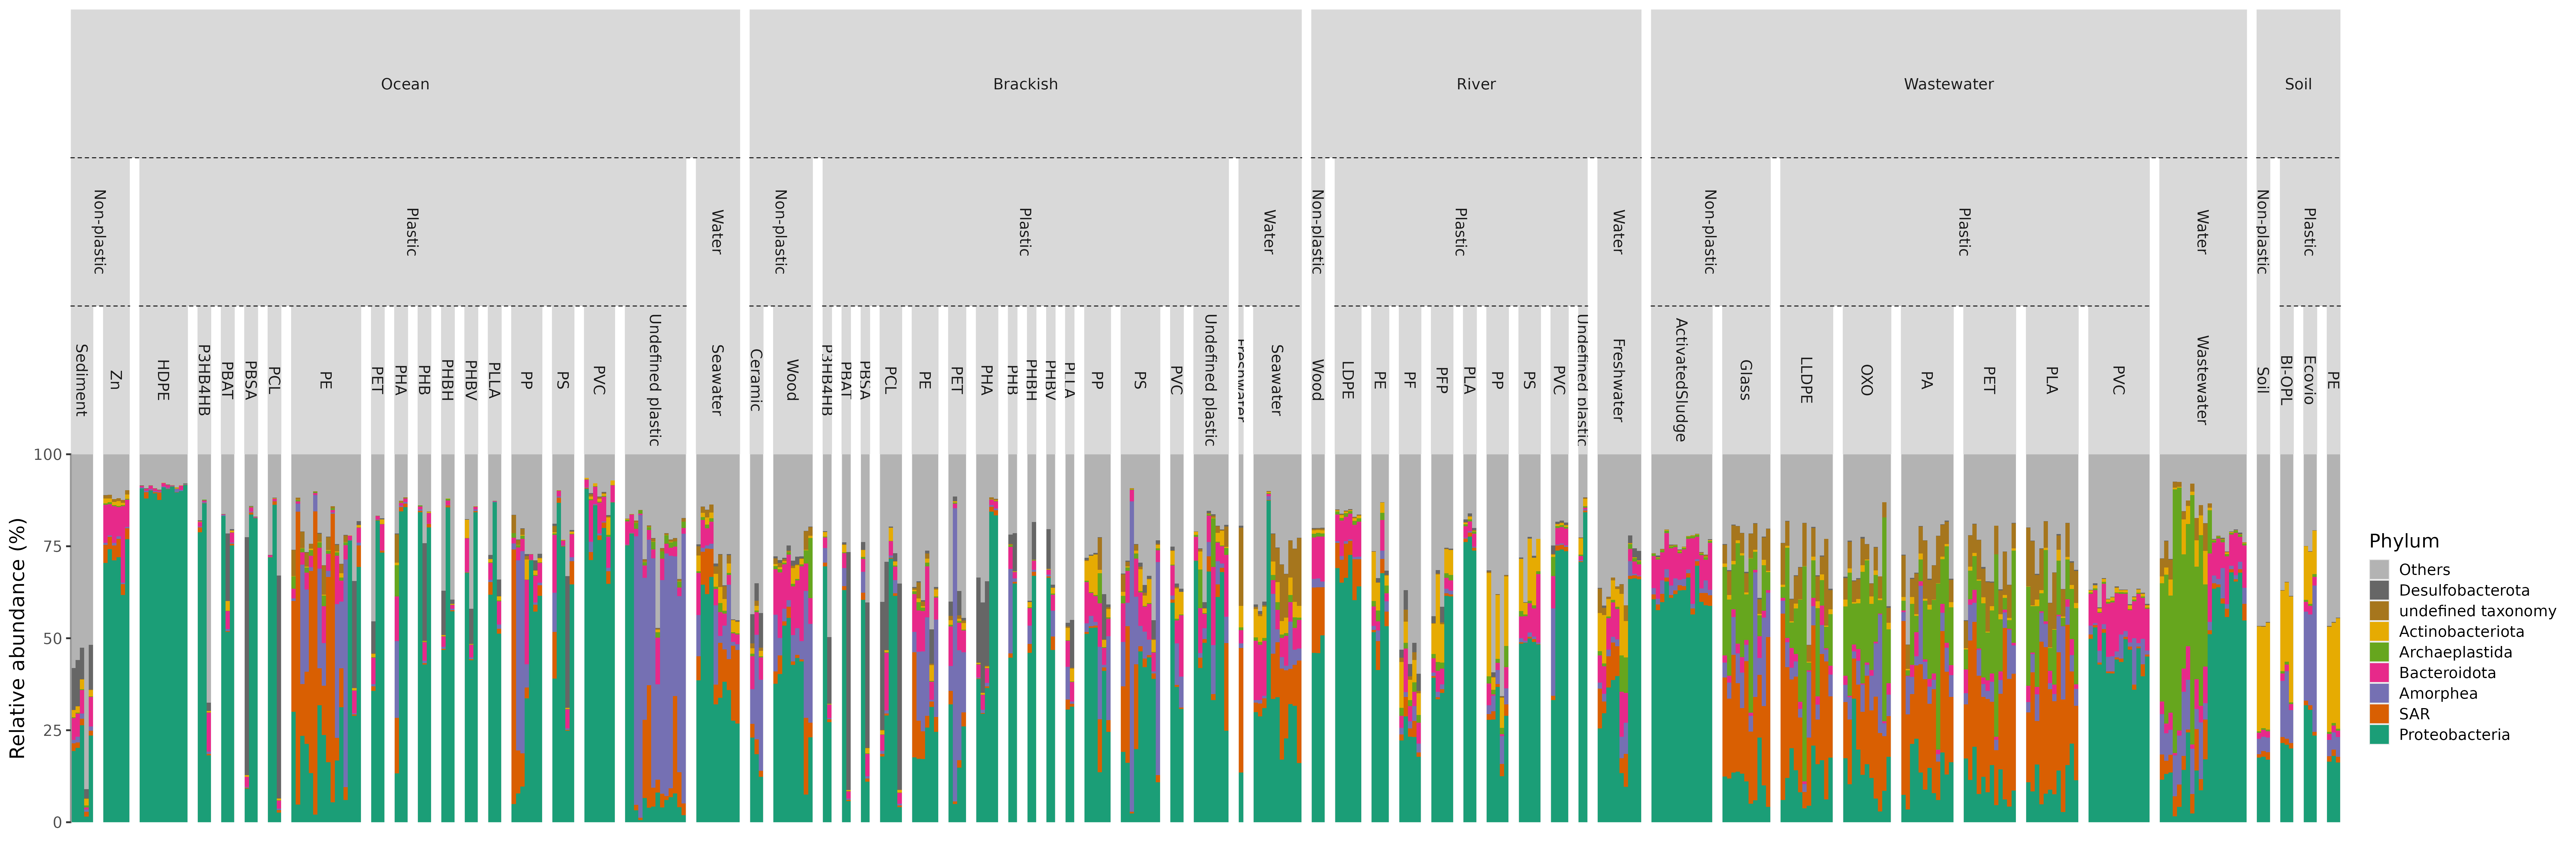
\includegraphics[width = 1.2\textwidth]{figure/tax_phylum_ecosystem_sampletype_substrate.png}
    \caption{Taxonomic abundance for all samples at the Phylum level, divided by ecosystem type, sampletype and substrate}
    \label{tax_plot_substrate}
\end{figure}

\begin{figure}[h]
    \centering
    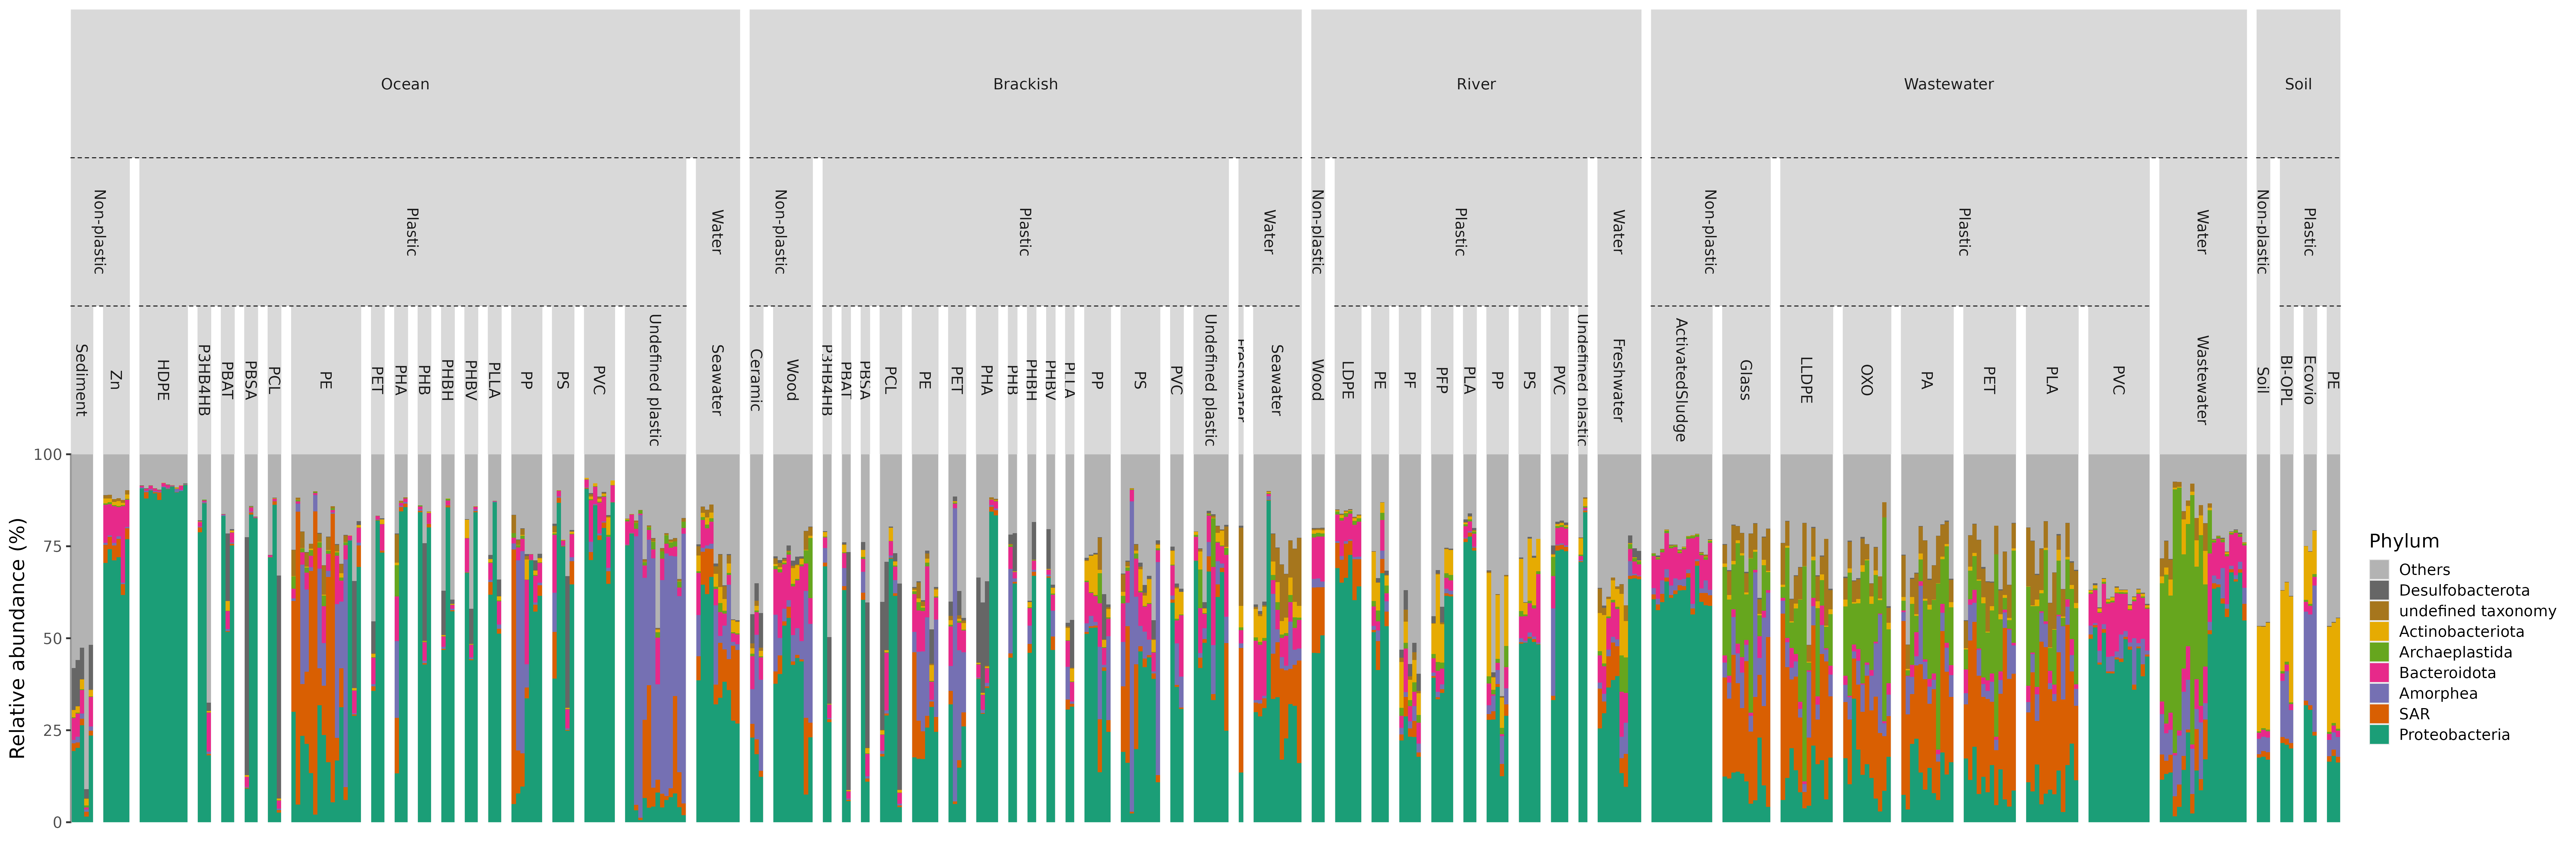
\includegraphics[width = \textheight, angle = 90]{figure/tax_phylum_ecosystem_sampletype_substrate.png}
    \caption{Same as last plot but rotated, rotate facet labels the other way if kept}
    \label{tax_plot_substrate_flip}
\end{figure}











